\chapter{Establishing laboratory methods and analytical tools to assess genome-wide chromatin accessibility in clinical samples}
\chaptermark{Establishment of methods to assess genome-wide chromatin accessibility}
\label{ch:Results1}


%%%%%%%%%%%%%%%%%%%%%%%%%%%%%%%%%%%%%%%%%%%%%%%%%%
\section{Introduction}
\subsection{Principle of ATAC-seq and compatibility with clinical samples}
Several techniques including DNase-seq, FAIRE-seq and MNase-seq have been used during the last few decades to map the accessible genome in different cell lines and some abundant sources of primary cells (reviewed in Chapter \ref{ch:Intro}). All these techniques require a large number of cells as input material, making them unsuitable for use in a clinical setting. The publication of ATAC-seq represented a revolution in the field to interrogate chromatin accessibility. ATAC-seq uses a hyperactive modification of the bacterial transposase Tn5 to perform simultaneous fragmentation and insertion of synthetic oligonucleotides (adapters) into native chromatin from 50,000 cells and also at single-cell resolution \parencite{Buenrostro2013, Buenrostro2015}. The Tn5 reaction incorporates, in a non-strand specific manner, adapters containing the complementary sequences to the i5-R1 and i7-R2 elements required for Illumina NGS. ATAC-seq provided a fast two-step protocol, not requiring cross-linking, enzyme titration or sonication, that was able to profile nucleosome-free DNA (fragments $\leq$150bp) and DNA spanning nucleosomes (fragments $>$150bp). ATAC-seq data can also be used to identify TF foot-printing as well as nucleosome positioning in the genome. This technique opened a new avenue to interrogate the chromatin landscape in clinical samples with limited input material as well as in rare cell populations, with a shorter preparation and results turn-over time.


\subsection{ATAC-seq limitations and advances in optimisation}  
Despite these advantages, early data from ATAC-seq revealed two major limitations, namely, a high percentage of mitochrondrial DNA tagged by the Tn5 enzyme, and insufficient sensitivity to detect all the accessible regions, partly due to high background noise \parencite{Corces2016, Sos2016}. An optimised version of the protocol specifically for haematopoietic cells, named Fast-ATAC, replaced the NP-40 detergent used in ATAC-seq with digitonin. This prevents solubilisation of the mitochondrial membrane, and performs lysis and transposition in a single step. This modification efficiently reduced the percentage of mitochondrial reads to approximately 10\% and increased the signal at annotated TSS, using only 5,000 cells as input material \parencite{Corces2016}. Optimisation of the ATAC-seq protocol for keratinocytes was also published by Bao and colleagues, where they performed the two ATAC-seq steps directly on the 96-well plate containing adherent NHEKs using an increased concentration of Tn5 in the transposition reaction \parencite{Bao2015}.

%Concomitantly, a more profound modification of the ATAC-seq protocol, known as transposome hypersensitive sites sequencing (THS-seq), was developed, incorporating newly designed adapters and genetic engineered Tn5, optimised transposition buffer and modified PCR amplification system \parencite{Sos2016}. The THS-seq protocol showed improved sensitivity and specificity for lower number of cells and small accessible regions compared to ATAC-seq at the cost of increased complexity and duration of the protocol.

The third generation of ATAC (in this thesis  ATAC will be used to refer to the technique regardless of the specific protocol), known as Omni-ATAC, was released in 2017 and offered a generic version of the protocol optimised to yield high quality data in any cell type and fresh or frozen tissue \parencite{Corces2017}. The Omni-ATAC protocol consisted of lysis, wash and transposition steps. In addition to the NP-40 and digitonin, used by the previous ATAC protocols, Omni-ATAC also included Tween-20 in the lysis buffer to improve cell permeabilisation. Comparison of Omni-ATAC with ATAC-seq and Fast-ATAC data demonstrated a higher variability in sample quality and sensitivity in the latter two protocols \parencite{Corces2017}. Moreover, Omni-ATAC achieved greater signal-to-noise ratios by modifying the transposition buffer. Notably, this versatile protocol represented a particular improvement in keratinocytes with data demonstrating the inability of ATAC-seq and Fast-ATAC to yield good quality data in this cell type \parencite{Corces2017}.  



\subsection{Challenges of ATAC data analysis}  
Although some guidelines for DHS data analysis were available, the release of the new ATAC methods also led to a need to adapt and develop additional tools and strategies for chromatin accessibility data analysis. In contrast to DNase-seq or FAIRE-seq data starting from high number of cells (minimum of 10x10$^6$ cells), ATAC-seq and Fast-ATAC showed lower signal-to-noise ratios and higher variability across samples. This required appropriate implementation of quality control measurements in order to confidently identify good quality samples prior to downstream analysis. Regarding peak calling in ATAC, different algorithms have been applied, with MACS2 being preferred by the majority of studies, including ENCODE (\url{https://www.encodeproject.org/atac-seq/})(Table \ref{tab:ATAC_comparative_methods}). The criteria for filtering out poor quality peaks in ATAC is another critical aspect, particularly for the libraries at the lower end of the quality spectrum. False discovery rate (FDR) has been the most widely applied criterion except for ENCODE data, where technical replicates are generated and irreproducible discovery rate (IDR) analysis is used to identify robust peaks (\url{https://www.encodeproject.org/atac-seq/}) (Table \ref{tab:ATAC_comparative_methods}). 


\begin{landscape}
\begin{center}
\renewcommand{\arraystretch}{0.7}	
\begin{longtable}[ht]{p{.20\textheight} p{.40\textheight} p{.40\textheight} p{.40\textheight}}
\caption[Summary table of ATAC analysis methodology for peak calling, filtering and differential analysis.]{\textbf{Summary table of ATAC methodology analysis for peak calling, filtering and differential analysis.} NA indicates the study did not perform or detail that aspect of the analysis. Alasoo \textit{et al.} 2018 was published in bioRxiv in 2017 and access to Turner \textit{et al.} 2018 work was also available earlier through collaboration in the WHG. Thus both publications were considered at the time of establishing the pipeline. $^{\ast}$ Access to ENCODE ATAC pipeline at \url{https://www.encodeproject.org/atac-seq/}.}
\label{tab:ATAC_comparative_methods} \\
\toprule
\textbf{Publication} & \textbf{Peak calling and filtering} & \textbf{Consensus peak list} & \textbf{Differential analysis} \\
\midrule
\midrule
Corces \textit{et al.} 2016 & MACS2 (-nomodel), peak summit extension $+/-$250bp, rank summits by p-value & Maximally significant non-overlapping peaks. & Quantile normalisation and unsupervised hierarchical clustering. \\
ENCODE$^{\ast}$  & MACS2 -nomodel, pairwise IDR analysis, filtering IDR$<$10\% & Choosing longest pairwise IDR filtered list or only peaks present in the two samples pseudoreplicates. & NA \\   
 &&&\\        
Turner \textit{et al.} 2018 	& MACS2 (-nomodel --q 0.01) & Merging all filtered called peaks from the different cell types. & \textit{De novo}: DiffReps with fragment size 50bp. \\             																																						
 &&&\\  
Alasoo \textit{et al.} 2018 & MACS2 (-nomodel -shift -25 -extsize 50 --q 0.01 &	Union of peaks from all conditions present in at least three samples of the same condition. & Peak based: TMM normalisation and lima voom (FDR$<$0.1).\\ 
 &&&\\  
Qu \textit{et al.} 2017 & ZINBA PP$>$0.99. & Merging of filtered peaks from each individual sample. & Quantile normalisation and peak based in house Pearson correlation method. \\	
 &&&\\  						
Rendeiro \textit{et al.} 2016 & MACS2 (-nomodel -extsize 147)	& Merge of peaks from all samples in an iterative process including permutations & Peak based: quantile normalisation and Fisher exact text (FDR$<$0.05). \\
 &&&\\  
Scharer \textit{et al.} 2016 & HOMER (-style dnase) & Merge of all overlapping peaks between all samples using HOMER mergePeaks & Peak based: TMM normalisation and edgeR package (FDR$<$0.05). \\														   
\bottomrule
%\medskip
\end{longtable}
\end{center}
\end{landscape}


The feasibility of generating ATAC data from low numbers of cells and clinical samples presents an opportunity to perform differential chromatin accessibility analysis between conditions, cell types or groups of patients and healthy control samples. The most common approach is a peak based strategy, which requires building a non-redundant and non-overlapping list of high quality peaks, counting the reads mapping to those locations and performing normalisation across samples before conducting differential analysis with microarray or RNA-seq based-methods. An alternative is known as the \textit{de novo} approach, used for ChIP data, which consists of using a sliding window to scan the genome and identify those regions showing read count differences between two groups of samples, avoiding peak calling bias \parencite{Shen2013}.     


\subsection{The challenge of working with clinical samples}

The opportunity to apply epigenetic assays to clinical samples has also highlighted a logistical problem. Often patient recruitment takes place at distant geographical locations or out of normal working hours. This requires the application of preservation methods that provide a snap shot of the \textit{in vivo} cellular characteristics and avoid introducing confounders. The main methods to preserve cell structure and DNA integrity involve cryopreservation or DNA-protein fixative compounds such as formaldehyde. Regarding preservation of pure cell populations, a study in motor neurons demonstrated that slow-cooling using DMSO but not snap-freezing maintained intact cell nuclei and chromatin organisation and overall yielded comparable ATAC-seq data to those generated in fresh neurons \parencite{Milani2016}. When working with mixed cell populations such as PBMCs, slow temperature cryopreservation with DMSO allows long term storage and also offers the flexibility of retrospective separation of distinct cell populations by FACS following thawing and recovery. However, in a mixed population such as PBMCs some cell types are more sensitive to cryopreservation and that may lead to distinct alterations in the chromatin accessibility landscape and gene expression profile. In terms of fixatives, the Oxford Genomic Centre at the WHG had incorporated the use of dithio-bis(succinimidyl propionate) (DSP) to stabilise cell samples for single-cell transcriptomic applications demonstrating only moderate differences from fresh samples profiles \parencite{Attar2018}. DSP is a reversible cross-linker of free amine groups that fixes proteins without damaging RNA and is compatible with microfluidics-based scRNA-seq systems, unlike formaldehyde fixation. DSP preservation does not require sample freezing after fixation and samples can undergo successful immuno-staining as well as FACS cell separation \parencite{Espina2013}. %Therefore DSP appeared as a very attractive candidate for short term preservation of clinical samples' PBMCs compatible with their use in single-cell transcriptomics and ATAC-seq assay.


%https://www.ncbi.nlm.nih.gov/pmc/articles/PMC545482/
%These two aspects make ATAC-seq a very versatile technique to interrogate the chromatin landscape in a clinical set-up, where sample availability and time-efficiency are key factors \parencite{Scharer2016,Qu2015,Qu2017}. Regardless of the strengths of this new technique, ATAC-seq sensitivity is not comparable to DNase-seq for some cell types and tissues, and further optimisations of the first released protocol by Buenrostro and colleagues have been implemented \parencite{Corces2016,Sos2016,Corces2017}. 

\subsection{Aims}

The aim of this chapter is to establish the ATAC protocols in the laboratory, perform a thorough optimisation of the methodological and analytical tools required to study chromatin accessibility in clinical samples of interest, and to determine the suitability of relevant methods for sample preservation to overcome the inherent logistical constraints of working with clinical samples.
 
The specific aims of this chapter are:
 
\begin{enumerate}
\item To establish an in-house pipeline to analyse ATAC data including quality control measurements, peak filtering and a method for differential analysis in order to maximise the use of available samples.
 
\item To investigate the effect of transposition time on sample quality in the ATAC-seq protocol.
 
\item To validate the reduction of mitochondrial DNA and improvement of signal in Fast-ATAC protocol compared to ATAC-seq.
 
\item To test and optimise ATAC-seq protocols in order to adapt them to the mapping of the chromatin accessibility landscape in psoriasis skin biopsies and in cultured primary keratinocytes.

\item To determine the effect of cryopreservation and DSP fixation on ATAC-seq data quality and on the overall chromatin accessibility landscape of CD14$^+$ monocytes and total CD4$^+$ (CD4$^+$) cells.
\end{enumerate}



%%%%%%%%%%%%%%%%%%%%%%%%%%%%%%%%%%%%%%%%%%%%%%%%%%
\section{Results}
%

\subsection{Establishment of an ATAC-seq data analysis pipeline}
A robust ATAC-seq data analysis pipeline was required as this was a new methodology \parencite{Buenrostro2013} for which established pipelines were not available at the time this work was undertaken. Such a pipeline requires appropriate quality control, peak calling and filtering, and a method for identification of differential chromatin accessibility between groups of samples. 

The most appropriate criteria and parameters to implement were investigated using ATAC-seq data generated for paired CD14$^+$ monocytes and CD4$^+$ T cells from three healthy individuals (referred as CTL1-3). This data corresponds to the fresh samples generated to test the effect of cryopreservation and fixation in the chromatin landscape, further detailed in section \ref{Core} (Table \ref{tab:Summary_all_cohorts}) and was appropriate to establish quality control measurements and the differential analysis approach later implemented for the study of psoriasis and PsA chromatin accessibility landscape (Chapters \ref{ch:Results2} and \ref{ch:Results3}). 


%At the time of the first ATAC-seq publication \parencite{Buenrostro2013}, well established protocols for complete processing and data analysis were lacking. Since then, several publications have implemented ATAC-seq and modifications of this protocol together with a wide range of data analysis strategies to answer different biological questions (Table \ref{tab:ATAC_comparative_methods}).In the process of analysing ATAC-seq data, several limiting aspects are encountered, including quality control assessment, peak calling and filtering, and identification of differential chromatin accessibility between groups of samples. Using the current knowledge in the field as well as custom analysis, the most appropriate criteria and parameters to implement in the in-house pipeline were established. For this purpose different types of analysis were performed using ATAC-seq data generated with the \parencite{Buenrostro2013} protocol in paired CD14$^+$ monocytes and total CD4$^+$ T cells (tCD4$^+$) from three healthy individuals (ATAC-seq fresh samples generated for \label{Core}). 


\subsubsection{Sample quality control}
%all of them downsamples to 30 million of reads, in order to facilitate the comparison across all of them.
The variability in performance of ATAC experiments and protocols requires appropriate quality control of the samples before proceeding with downstream differential analysis. ATAC-seq fragment size distribution was analysed in each library containing between 25 and 30 million reads. The observed fragment size distribution demonstrated nucleosome periodicity protecting the DNA during the transposition event (Figure \ref{figure:QC_ATAC}A) and indicated chromatin integrity, one of the requirements for good quality ATAC libraries. All six libraries showed appropriate nucleosome periodicity (every $\sim$200bp) up to 600bp, clearly distinguishing chromatin organisation into mono-, di- and tri-nucleosomes. Some variation in the relative intensity of nucleosome-free fragments (NFF) ($\leq$147bp, approximately) compared to nucleosome-bound DNA was seen across samples. However, NFF were clearly distinguished in all of the samples, which is considered a compulsory feature for ATAC-seq libraries to pass quality control, according to ENCODE recommendations (\url{https://www.encodeproject.org/atac-seq/})(Table \ref{tab:ATAC_comparative_methods}).

Another quality control measurement that was investigated and implemented was the enrichment of ATAC-seq signal over a random background of reads across all the TSSs identified for Ensembl genes (Figure \ref{figure:QC_ATAC}B). This is a useful measure as nucleosome repositioning and an increase in chromatin accessibility occur at the TSS to allow TF binding and initiation of gene transcription. Fold-enrichment signals over the TSS ranged from 5 to 7 for the CD4$^+$ samples, and were much higher (17 to 20) in the CD14$^+$ samples. The lower sample quality of the CD4$^+$ compared to CD14$^+$ samples indicated by the TSS enrichment values were further evidenced by visualising the ATAC-seq read pile up at the promoters of the glyceraldehyde-3-phosphate dehydrogenase (\textit{GAPDH}) and the NOP2 Nucleolar Protein (\textit{NOP2}) gene, showing more background reads and lower signal for the CD4$^+$ samples (Figure \ref{figure:QC_ATAC}C).
	
As part of the quality control assessment, the percentage of mitochondrial reads and the fraction of reads in peaks (FRiP) were also investigated (Table \ref{tab:ATAC_MT_fraction_reads_in_peaks}). FRiP score is an alternative to TSS enrichment for assessing the background signal in different types of assays that are based on peak calling, including ChIP-seq.

\begin{figure}[htbp]
\centering
\begin{subfigure}[b]{0.45\textwidth}
\centering
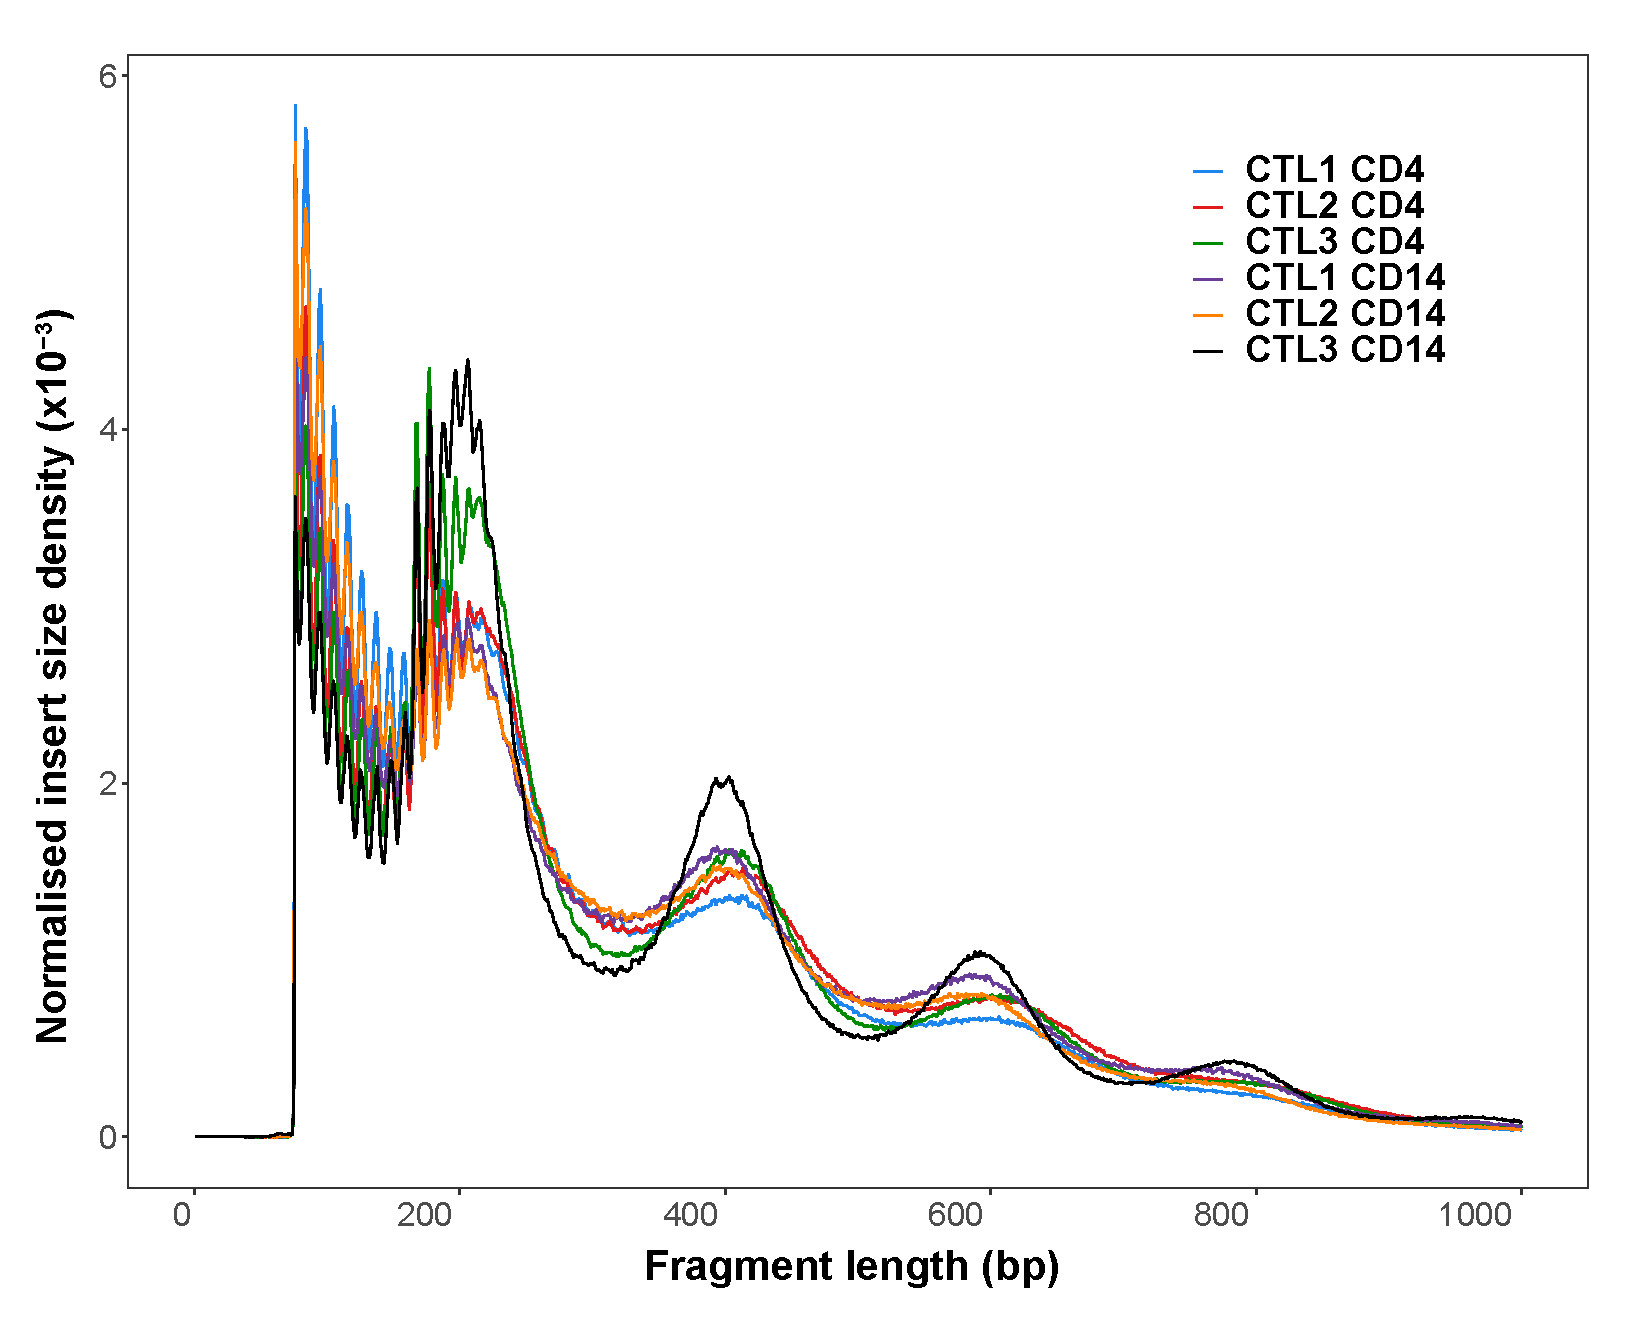
\includegraphics[width=\textwidth]{./Results1/pdfs/ATAC_Core_fresh_CD4_CD14_frag_size_distribution}
\caption{\textbf{}}
\end{subfigure}%
\begin{subfigure}[b]{0.45\textwidth}
\centering
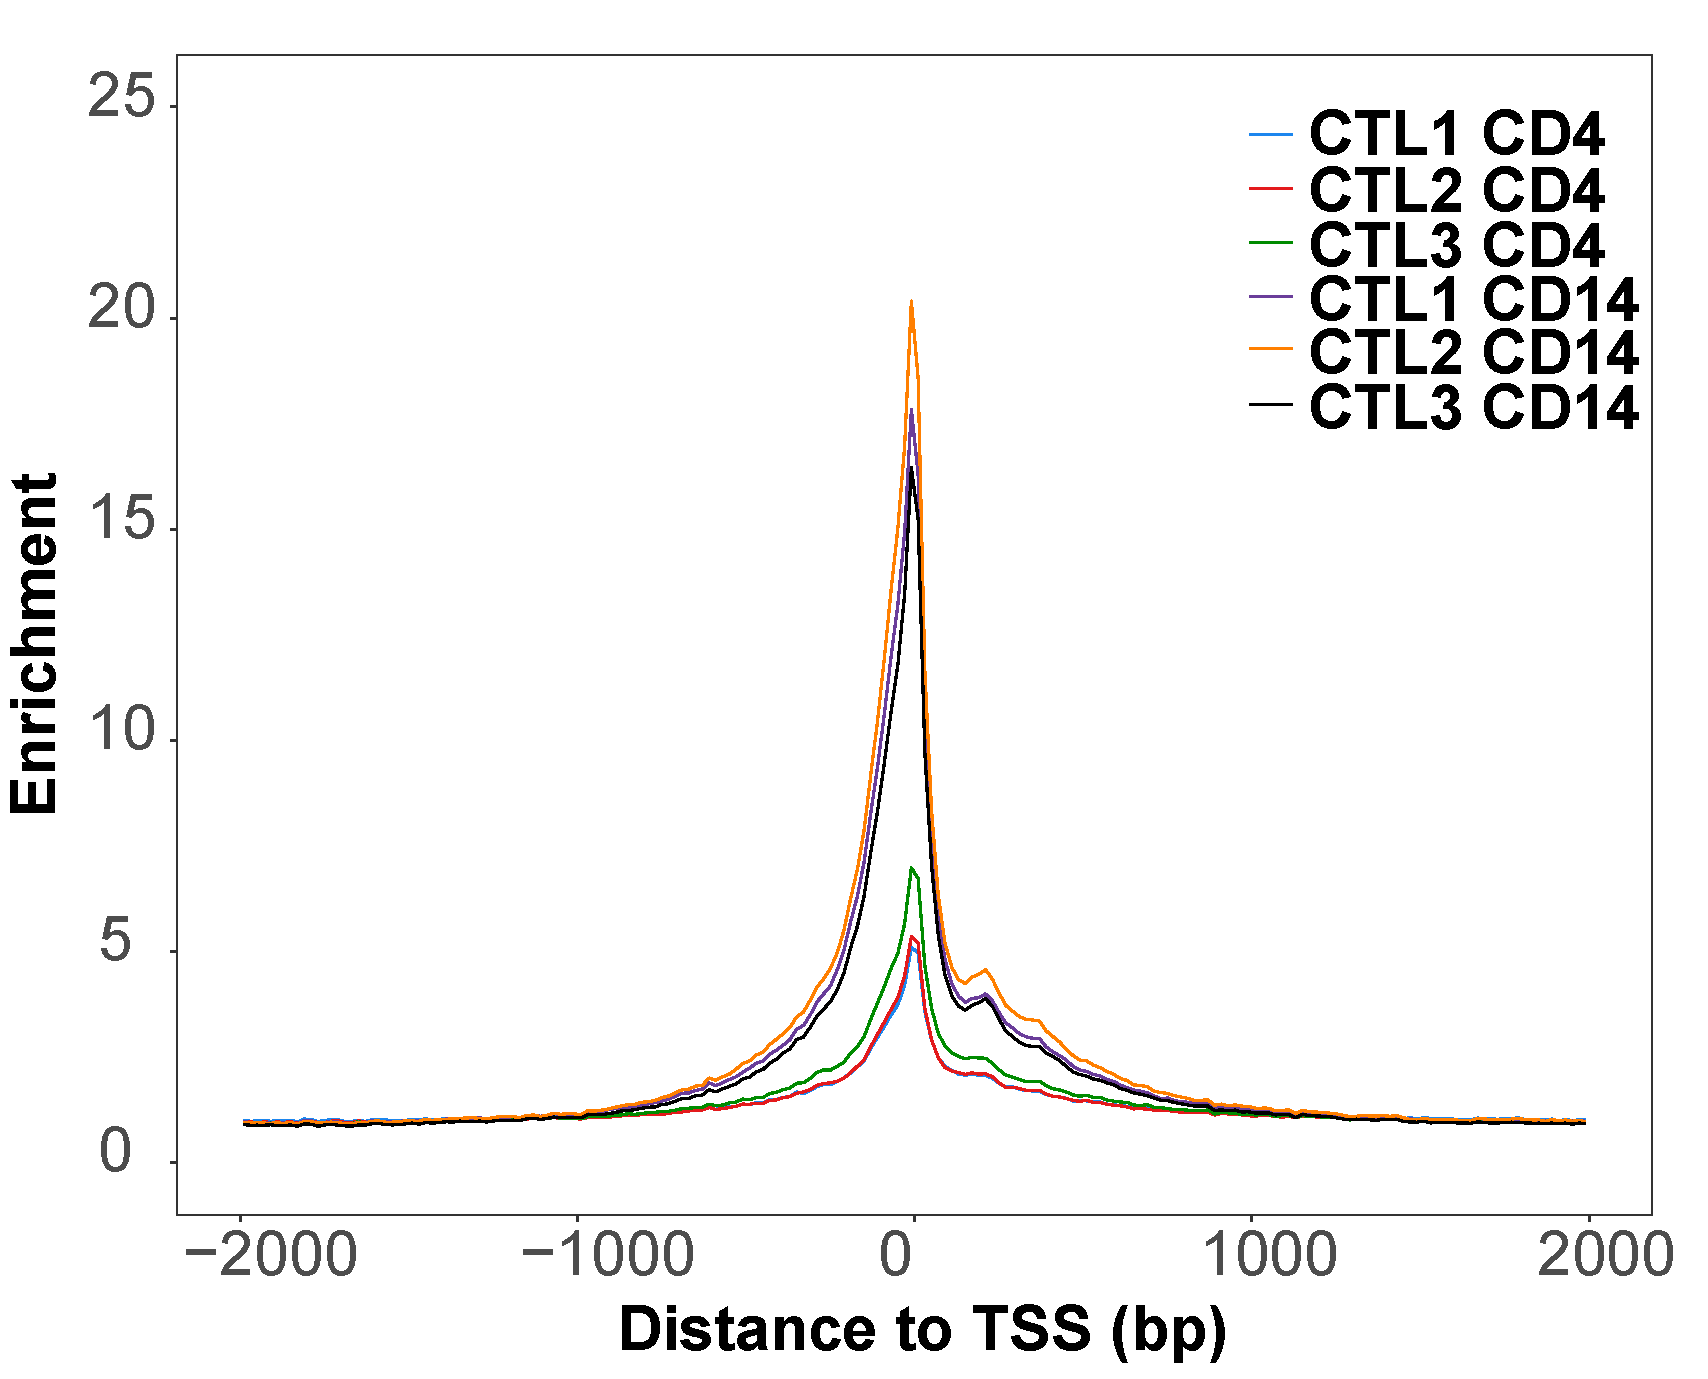
\includegraphics[width=\textwidth]{./Results1/pdfs/TSS_enrichment_Core_fresh_CD4_CD14}
\caption{\textbf{}}
\end{subfigure}
\begin{subfigure}[b]{0.6\textwidth}
\centering
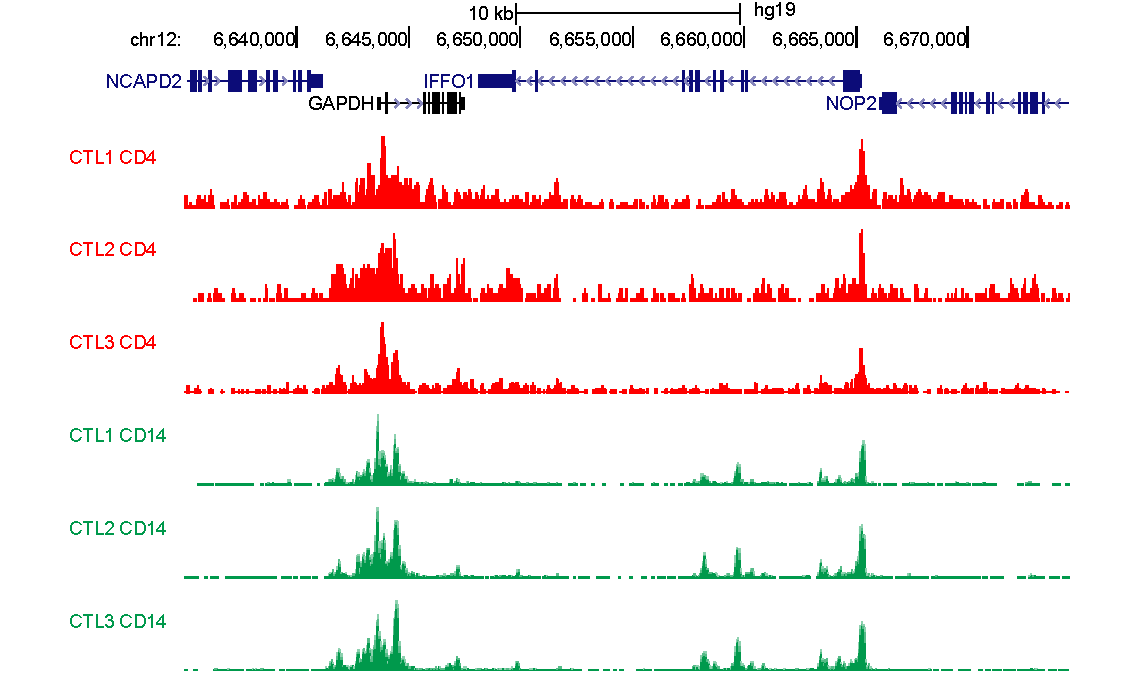
\includegraphics[width=\textwidth]{./Results1/pdfs/ATAC_Core_CD4_CD14_fresh_GAPDH}
\caption{\textbf{}} % to add text to the figure name
\end{subfigure}
\caption[Measurements for quality control assessment in ATAC-seq samples]{\textbf{Measurements for quality control assessment in ATAC-seq samples.} For each of the CD14$^+$ monocytes and CD4$^+$ samples used to establish the ATAC analysis pipeline quality control measures shown are (A) density distribution of ATAC-seq fragment sizes, (B) enrichment of ATAC-seq fragments across the TSS of all Ensembl genes and (C) UCSC Genome Browser view illustrating the ATAC-seq normalised read density (y-axis) at the promoters of \textit{GAPDH} and \textit{NOP2} genes. CD14$^+$ monocytes and CD4$^+$ tracks are colour-coded in green and red, respectively.}
\label{figure:QC_ATAC}
\end{figure} 

Positive correlation between the TSS fold-change enrichment and FRiP was observed and suggested that both are appropriate inter-dependent quality control measures to evaluate sample noise. For the six samples analysed here, mitochondrial content varied between (14.9-43.3\%), was higher in CD14$^+$ than in CD4$^+$ cells and was not directly related to any of the other quality control measurements. Therefore, mitochondrial reads in this range did not appear to reflect sample quality and the main issue related to the need for deeper sequencing to achieve the desired number of non-mitochondrial reads for downstream analysis.

 

\begin{table}[htbp]
%\setlength{\tabcolsep}{20pt} only to stretch the columns if you want
%\renewcommand{\arraystretch}{1.5}
\centering
\begin{tabular}{@{} c c c}
\toprule
\textbf{Sample} & \textbf{\% mitochondrial reads} & \textbf{Fraction of reads in peaks} \\
\midrule
\midrule
CTL1 CD4 & 14.9 & 9.8 \\
CTL2 CD4 & 30.5 & 11.2 \\
CTL3 CD4 & 28.8 & 11.6 \\
CTL1 CD14 & 43.3 & 32.2 \\
CTL2 CD14 & 36.8 & 57.0 \\
CTL3 CD14 & 37.6 & 49.9 \\
\bottomrule
\end{tabular}
\medskip %gap
\caption[ATAC-seq percentage of mitochondrial reads and fraction of reads in called peaks (FRiP).]{\textbf{ATAC-seq percentage of mitochondrial reads and fraction of reads in called peaks (FRiP).} The percentage of mitochondrial reads was calculated over the total number of sequencing reads (before filtering). FRiP was calculated as the proportion of ATAC-seq fragments overlapping significant peaks with standard filtering for all the samples (FDR$<$0.01).}
\label{tab:ATAC_MT_fraction_reads_in_peaks}
\end{table}



Both TSS and FRiP are appropriate signal-to-noise measures, with recommended threshold values from ENCODE and Alasoo and colleagues (Alasoo \textit{et al.} 2018 and previously published in bioRxiv in 2017) being FRiP between 10-20\% and TSS between 6-10. Importantly ENCODE has recently prioritised the use of TSS over FRiP as a more stable measure to determine noise and therefore this was the chosen measure for this thesis. In summary from this analysis, all six samples showed appropriate ATAC-seq patterns of fragment size distribution, FRiP and TSS, with the exception of CD4$^+$ CTL1 and CTL2, being borderline for the 6 fold-enrichment TSS threshold. 
%Importantly, this differences in the enrichment around the TSS successfully recapitulated the differences observed in the ATAC-seq density signal of the UCSC Genome Browser tracks between the CD14$^+$ and CD4$^+$ samples. These differences in ATAC-seq quality observed in these samples reflected the variability in performance of ATAC-seq and were useful in determining the influence of borderline sample quality in downstream analysis in order to choose the most robust strategy maximising the use of precious clinical samples. 



\subsubsection{Peak calling and filtering}
\label{peak_filtering}
Next, criteria for peak calling and filtering were investigated. Although different peak callers have been used to analyse ATAC-seq data, MACS2 has been the preferred algorithm by ENCODE and most publications at the time of this thesis (Table \ref{tab:ATAC_comparative_methods}). MACS2 was initially developed for ChIP data, but has also been used for DHS and ATAC-seq disabling the model option and manually setting the shift (--shift) and extension size (--extsize) parameters, which refer to the number of bp and direction for the reads to be shifted and the number of bp for them to be extended, respectively. Since the --extsize should correspond to the average fragment size, this was set to 200bp, the average fragment size calculated for the ATAC-seq libraries in this project. The --shift was set to -100, as it is recommended to be -1/2 of the fragment size when analysing chromatin accessibility data. 

A systematic analysis of the effect of sequencing depth and the sample quality on peak calling was conducted to better understand the effect of both variables on the downstream analysis. For each of the six samples, random sub-sampling of reads was performed in every 5 million increment, ranging from 5 to 30 total million reads, followed by peak calling with arbitrary filtering for false discovery rate (FDR)$<$0.01. The number of called peaks passing filtering showed a steady increase with read depth  (Figure \ref{figure:Peak_calling_versus_depth_ATAC}A), beginning to plateau at approximately 25 million reads (Figure \ref{figure:Peak_calling_versus_depth_ATAC}B). Moreover, lower number of peaks were detected in CD4$^+$ samples compared to CD14$^+$ monocytes when using standard  FDR$<$0.01 filtering, highlighting the influence of sample quality on the total number of called peaks. Interestingly, sample quality as measured by FRiP (which relies on peak calling) showed very small changes with read depth and was stable from 15 million reads onwards for all six samples (Figure \ref{figure:Peak_calling_versus_depth_ATAC}C), similarly to TSS (Figure \ref{figure:Peak_calling_versus_depth_ATAC}D). This confirmed that measurement of sample quality using FRiP or TSS was not affected by the sequencing depth.

\begin{figure}[H]
\centering
\begin{subfigure}{0.48\textwidth}
\centering
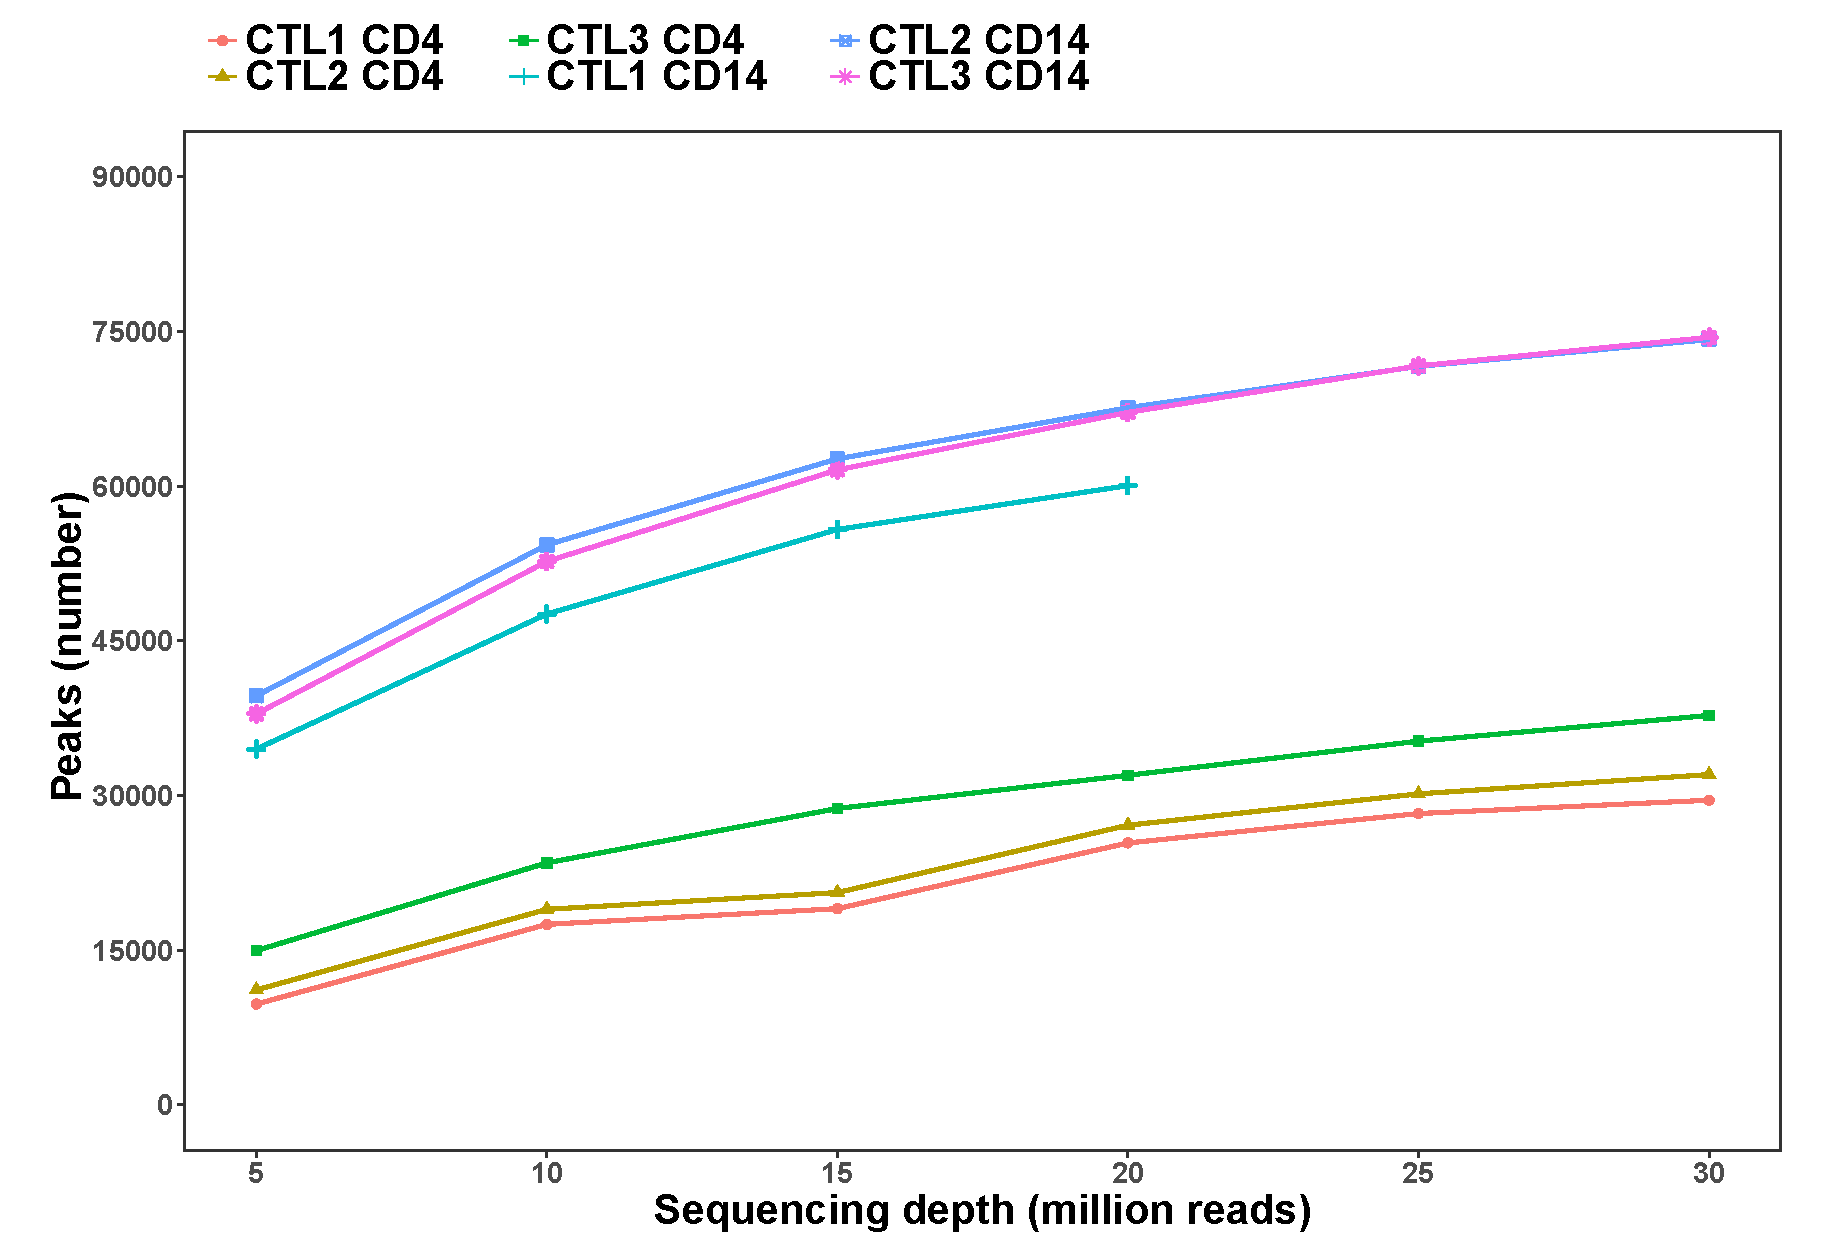
\includegraphics[width=\textwidth]{./Results1/pdfs/ATAC_Core_fresh_CD4_CD14_num_peaks_vs_depth}
\caption{\textbf{}}
% The percentage sign indicated that the other subfig goes side by side
\end{subfigure} %
\begin{subfigure}{0.48\textwidth}
\centering
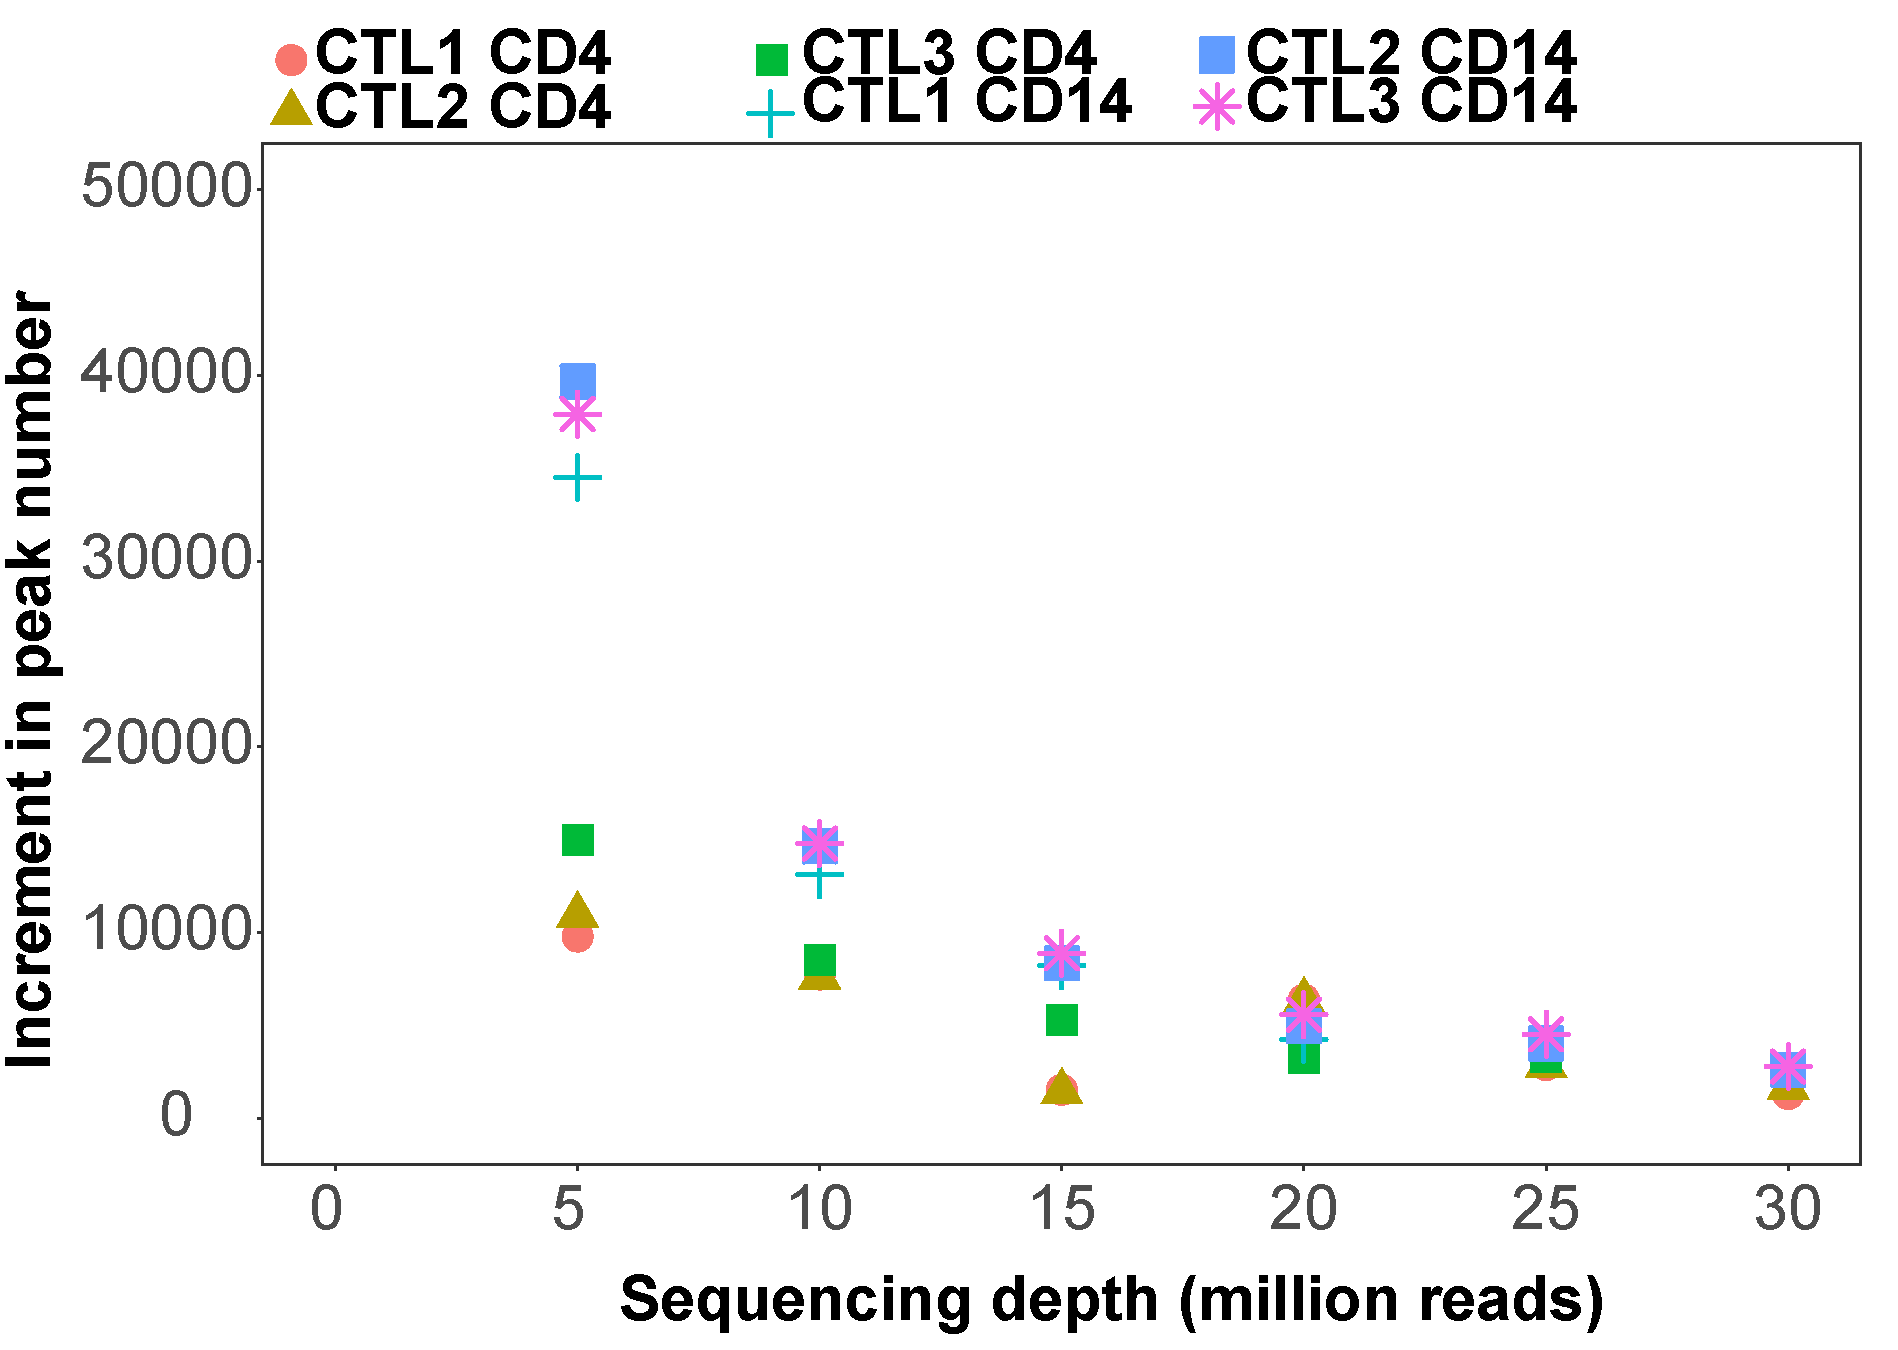
\includegraphics[width=\textwidth]{./Results1/pdfs/ATAC_Core_fresh_CD4_CD14_increment_num_peaks_vs_depth}
\caption{\textbf{}}
\end{subfigure} 
\begin{subfigure}{0.48\textwidth}
\centering
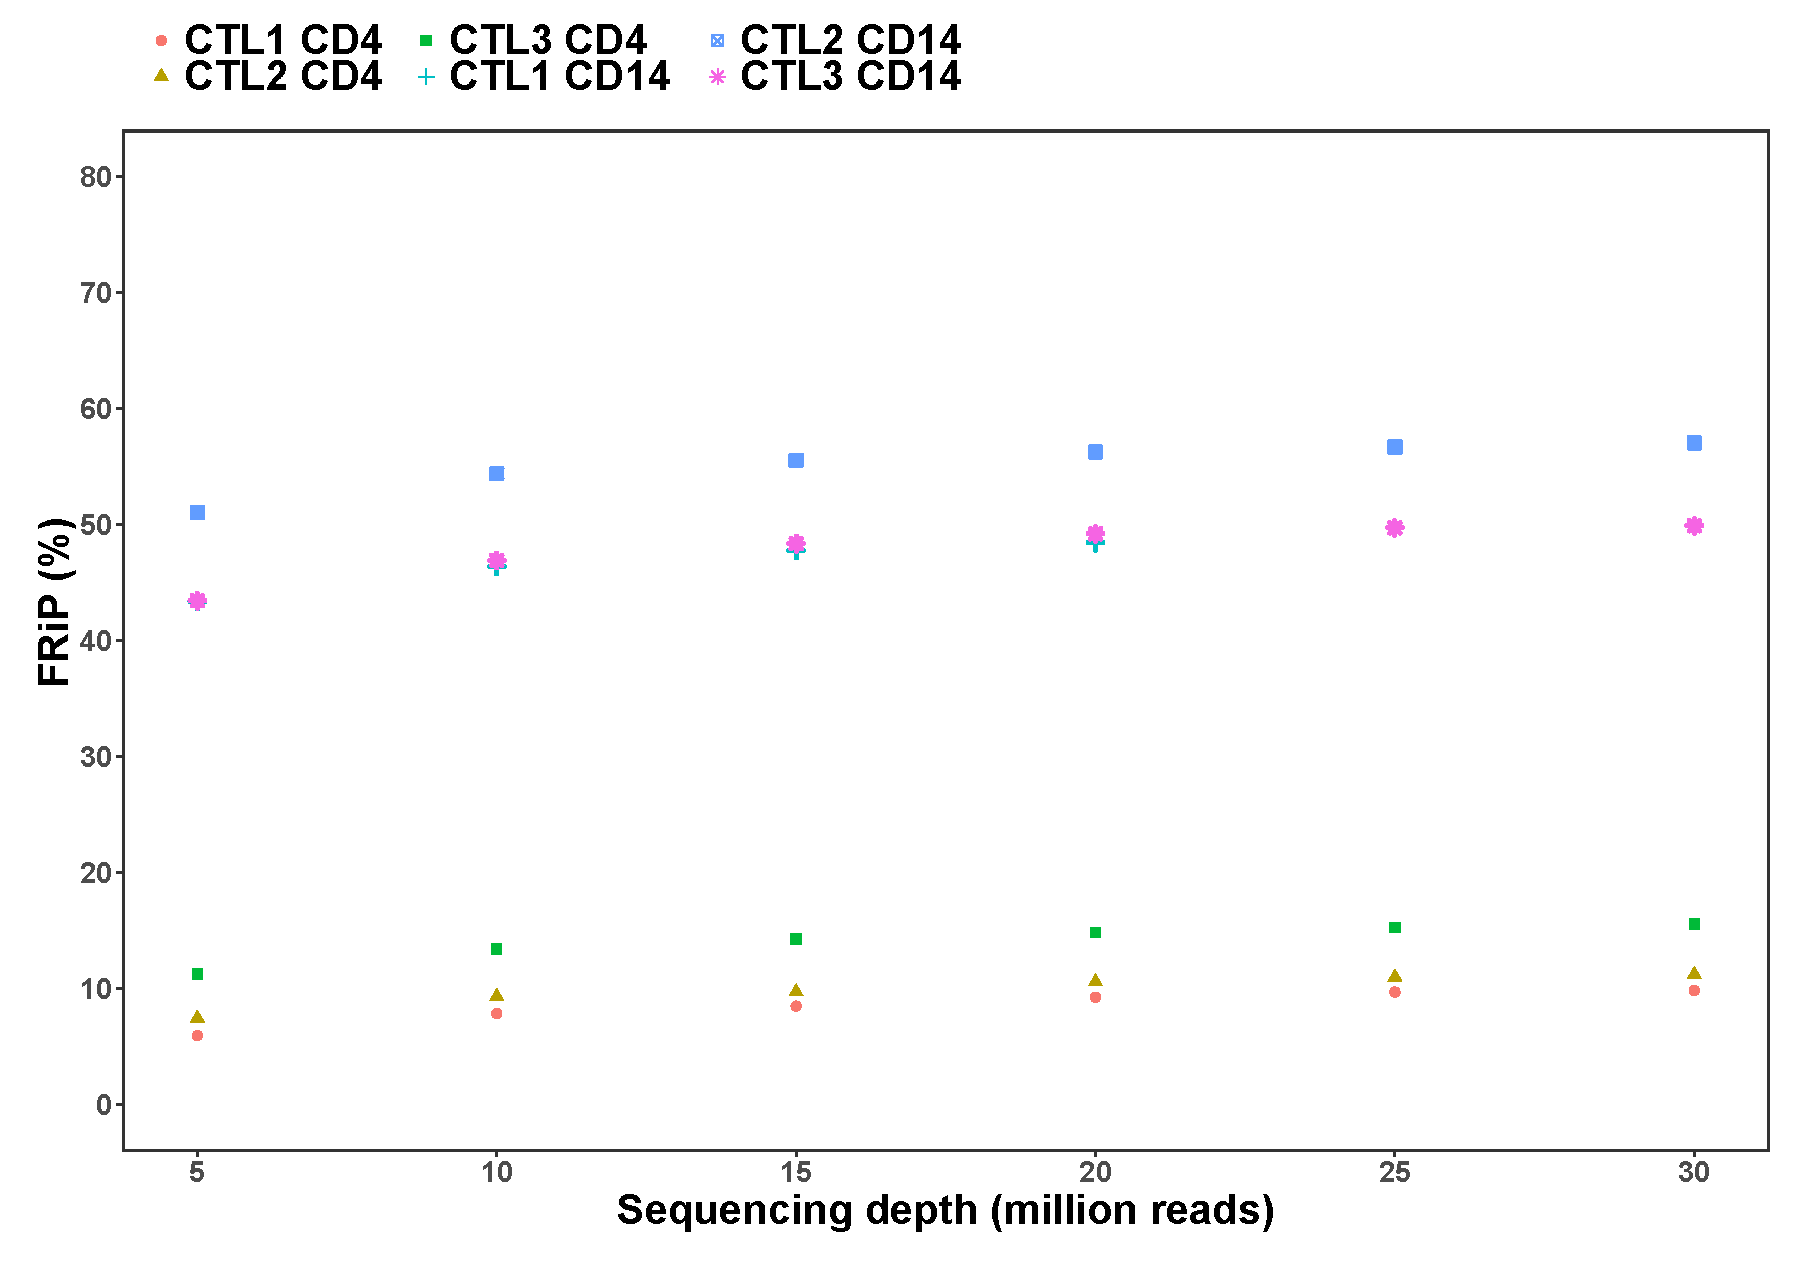
\includegraphics[width=\textwidth]{./Results1/pdfs/ATAC_Core_fresh_CD4_CD14_frac_reads_in_peaks_vs_depth}
\caption{\textbf{}}
\end{subfigure}%
\begin{subfigure}{0.48\textwidth}
	\centering
	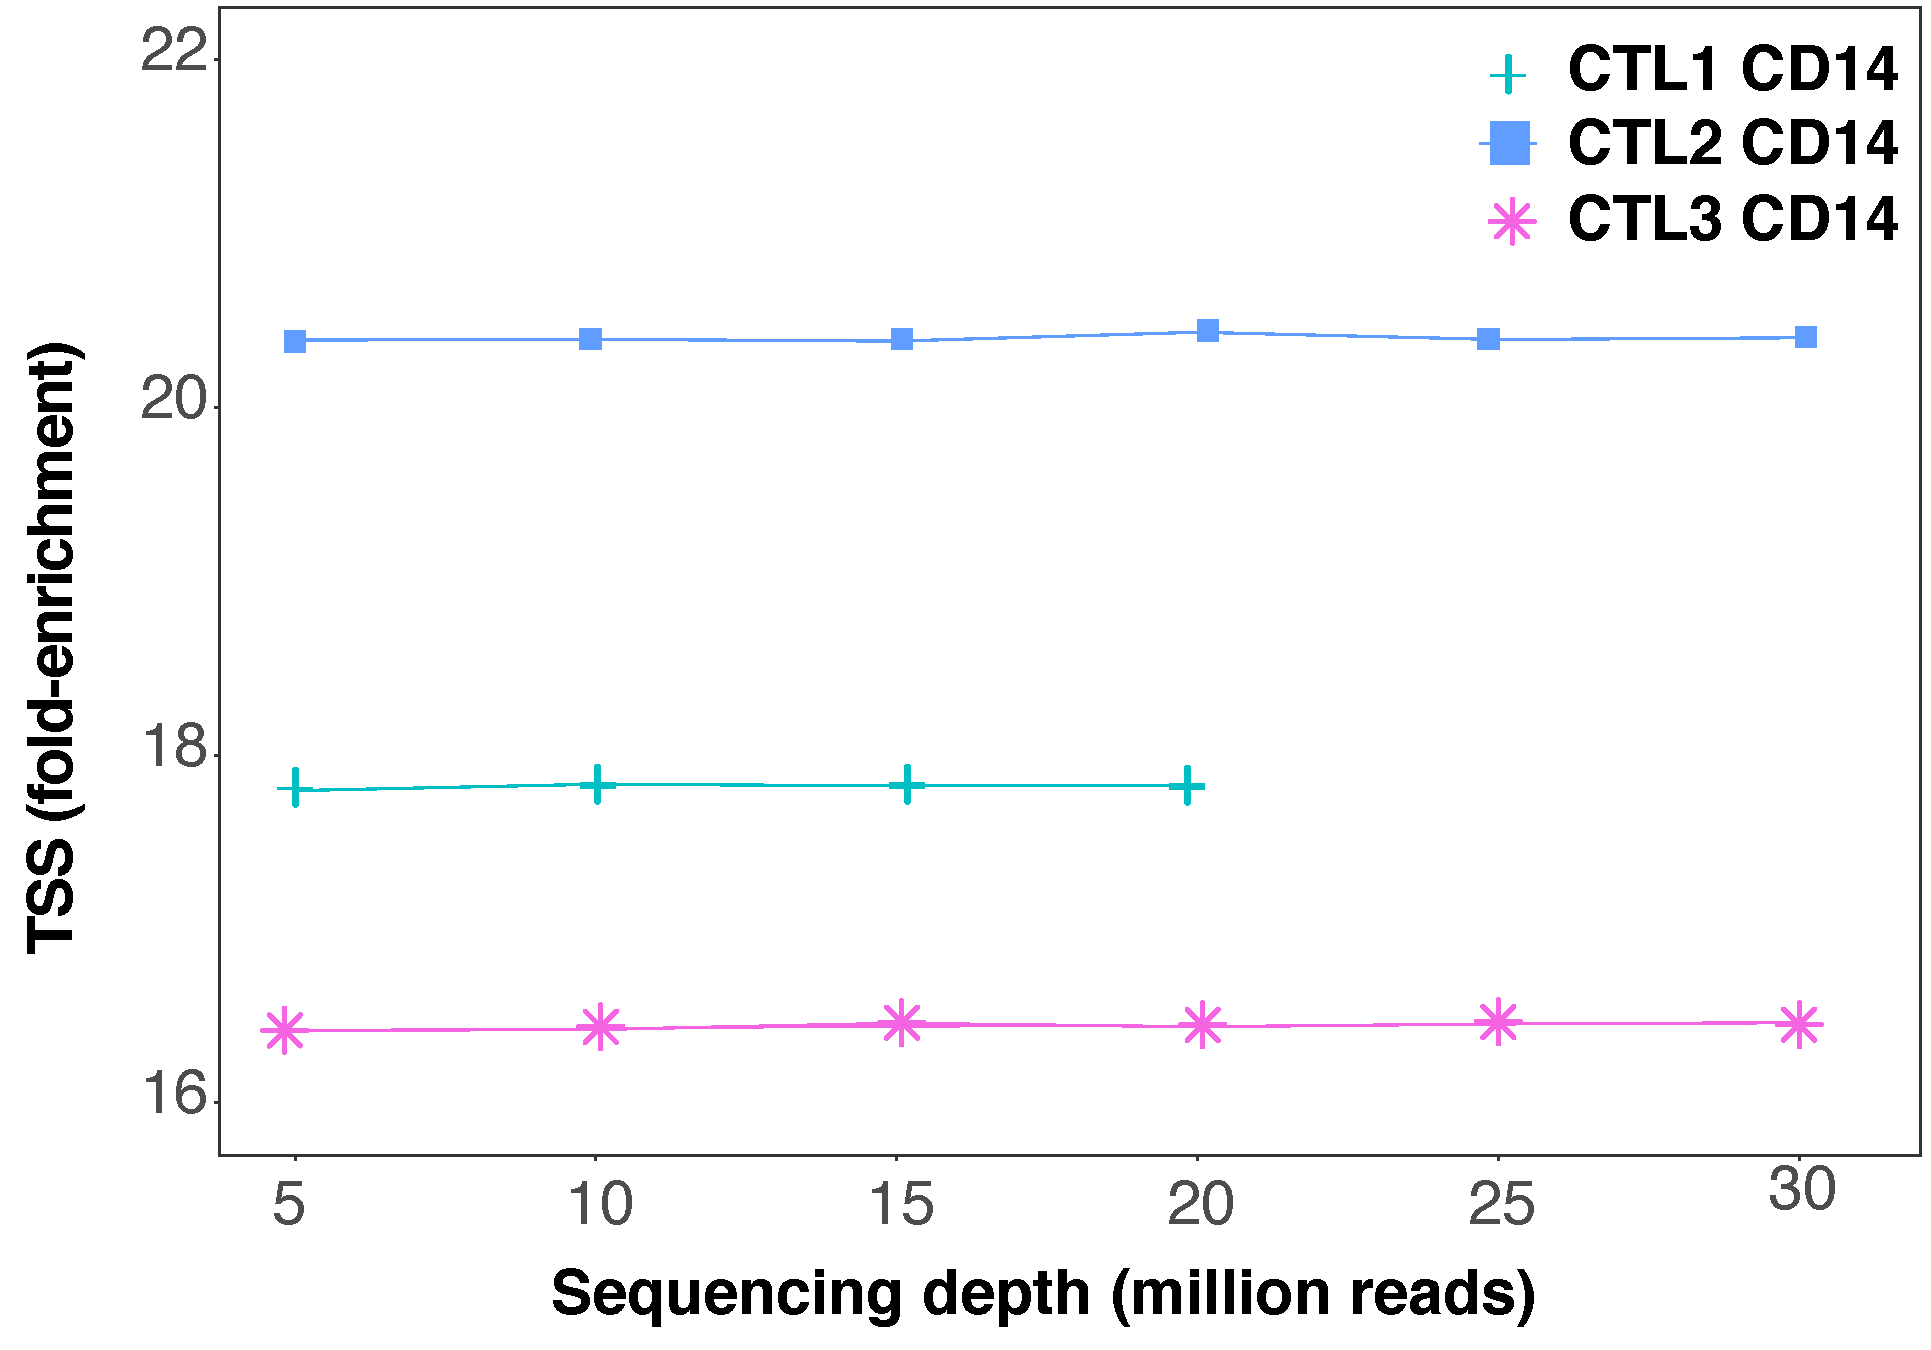
\includegraphics[width=\textwidth]{./Results1/pdfs/Core_TSS_vs_sequencing_depth_CD14}
	\caption{\textbf{}}
\end{subfigure}
\caption[FRiP and peak calling at different sequencing depths in ATAC-seq libraries.]{\textbf{FRiP and peak calling at different sequencing depths in ATAC-seq libraries.} For a series of sequencing depths (from 5 to 30 million reads after filtering) representation of (A) number of called peaks (standard filtering using FDR$<$0.01, (B) the increment on the number of called peaks and (C) FRiP and (D) TSS as a function of the sequencing coverage in CD4$^+$ and/or CD14$^+$ samples.}
\label{figure:Peak_calling_versus_depth_ATAC}
\end{figure} 


For peak filtering, an arbitrary FDR$<$0.01 in MACS2 is typically used (Table \ref{tab:ATAC_comparative_methods}) but may not remove low quality peaks equally successfully in lower quality samples and does not take into account the reproducibility of the called peaks. Thus IDR was used to experimentally identify the most appropriate p-value threshold to filter the called peaks in each individual sample. Filtered reads from each sample were partitioned in half to create two pseudoreplicates, peaks were called in each pseudoreplicate and the percentage of peaks sharing IDR rank position when filtered at decreasing p-values was calculated (Figure \ref{figure:Peak_calling_IDR_filtering_and_chrom_stated_ATAC}A and B). This strategy was tested across a range of total read counts (as above) to determine the effect of sequencing depth on the suitability of this peak calling filtering approach. The optimal p-value giving the largest percentage of IDR shared peaks between the two pseudoreplicates varied more erratically when the sequencing depth was lower than 10 million reads (Figure \ref{figure:Peak_calling_IDR_filtering_and_chrom_stated_ATAC}A and B), suggesting this analysis was not appropriate for lower read depths. This variation was more pronounced and extended in CD4$^+$ T cells, which had lower TSS values compared to CD14$^+$ monocytes (Figure \ref{figure:Peak_calling_IDR_filtering_and_chrom_stated_ATAC}A and B). The shape of the curves were also influenced by the sample quality. For appropriate sequencing depth (15-20 million reads), the CD14$^+$ monocytes (TSS enrichment $\geq$10) samples presented a profile reaching a single maximum of shared IDR peaks for a particular filtering p-value (Figure \ref{figure:Peak_calling_IDR_filtering_and_chrom_stated_ATAC}B), which was -log10 p-value 8 in all three samples (data not shown). In contrast, the same analysis in CD4$^+$ samples reached two local maxima (Figure \ref{figure:Peak_calling_IDR_filtering_and_chrom_stated_ATAC}A). 



\begin{figure}[htbp]
\centering
\begin{subfigure}{0.50\textwidth}
\centering
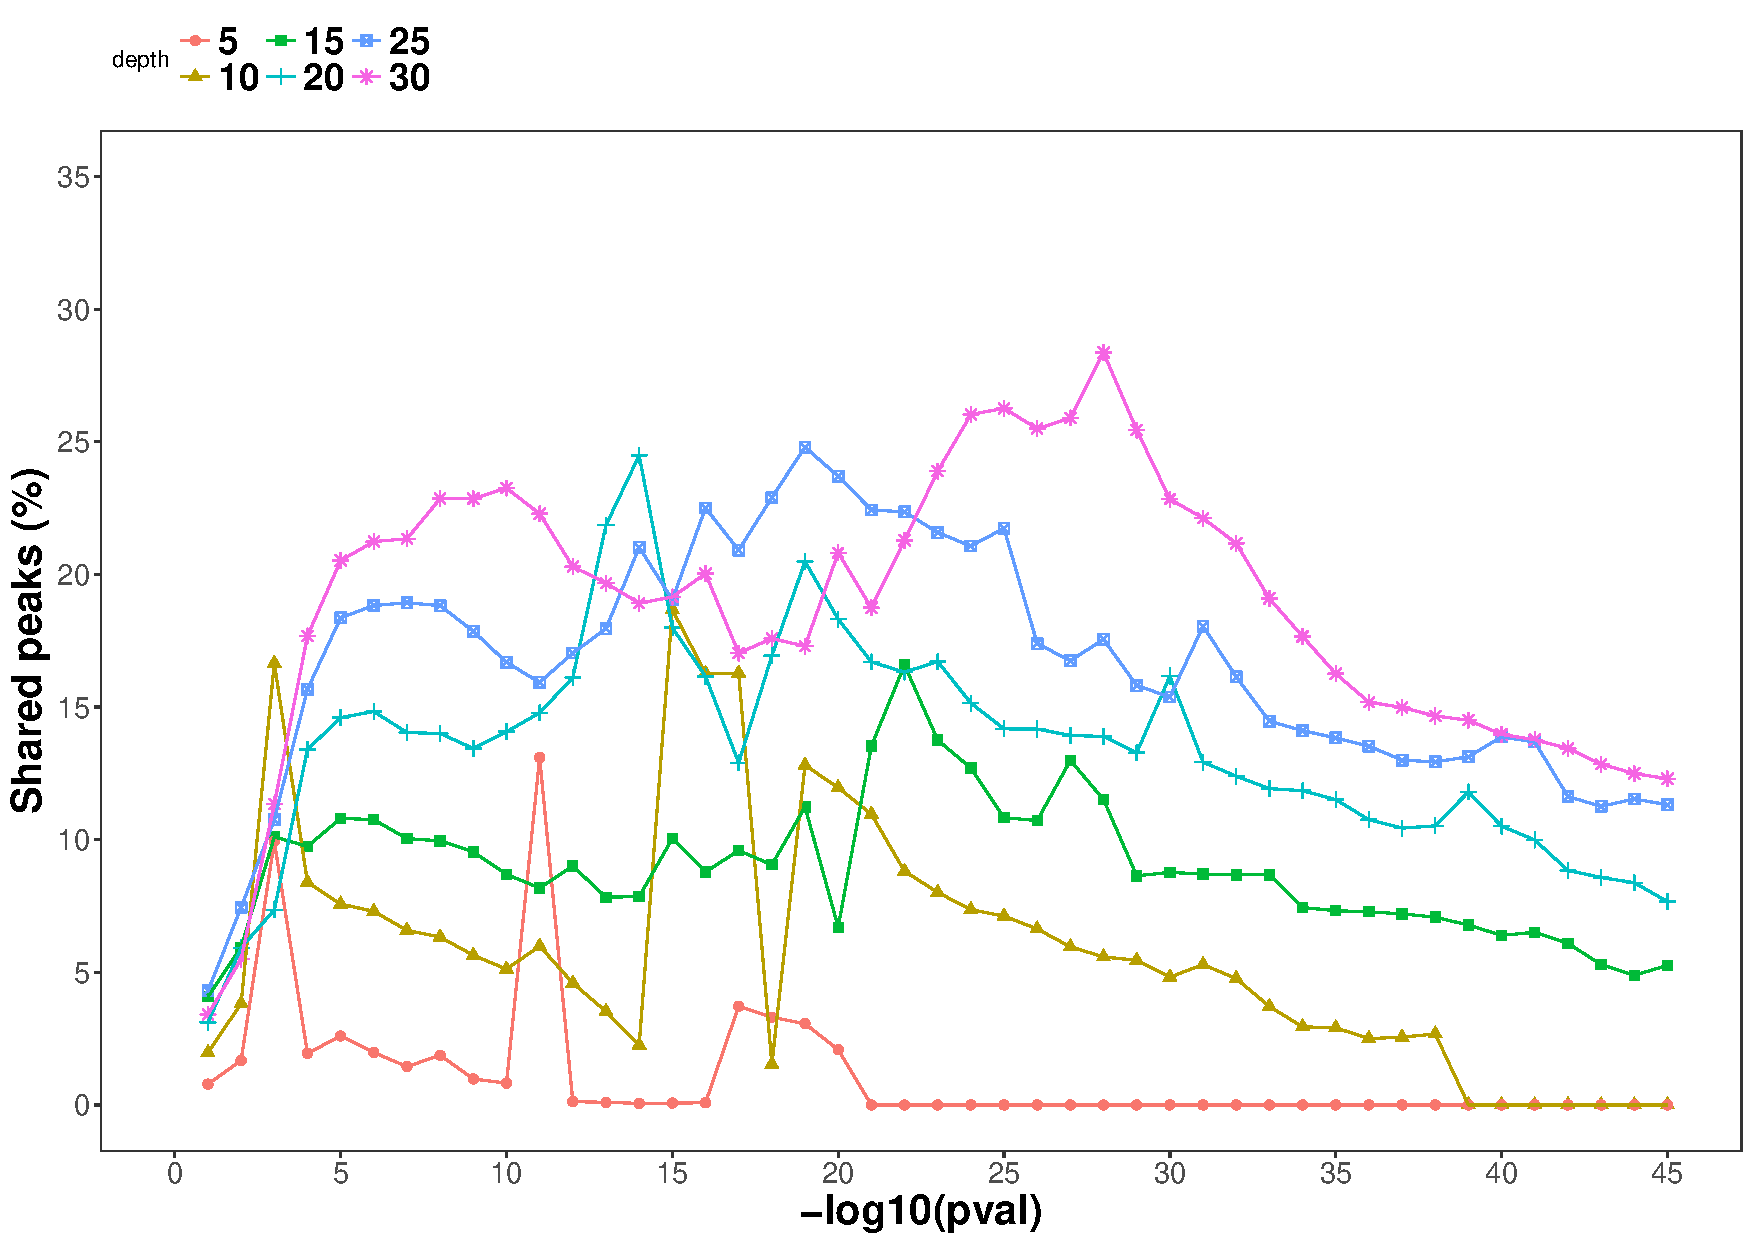
\includegraphics[width=\textwidth]{./Results1/pdfs/ATAC_Core_fresh_CTL2_CD4_shared_peaks_IDR_vs_pval}
\caption{\textbf{}}
% The percentage sign indicated that the other subfig goes side by side
\end{subfigure}%
\begin{subfigure}{0.50\textwidth}
\centering
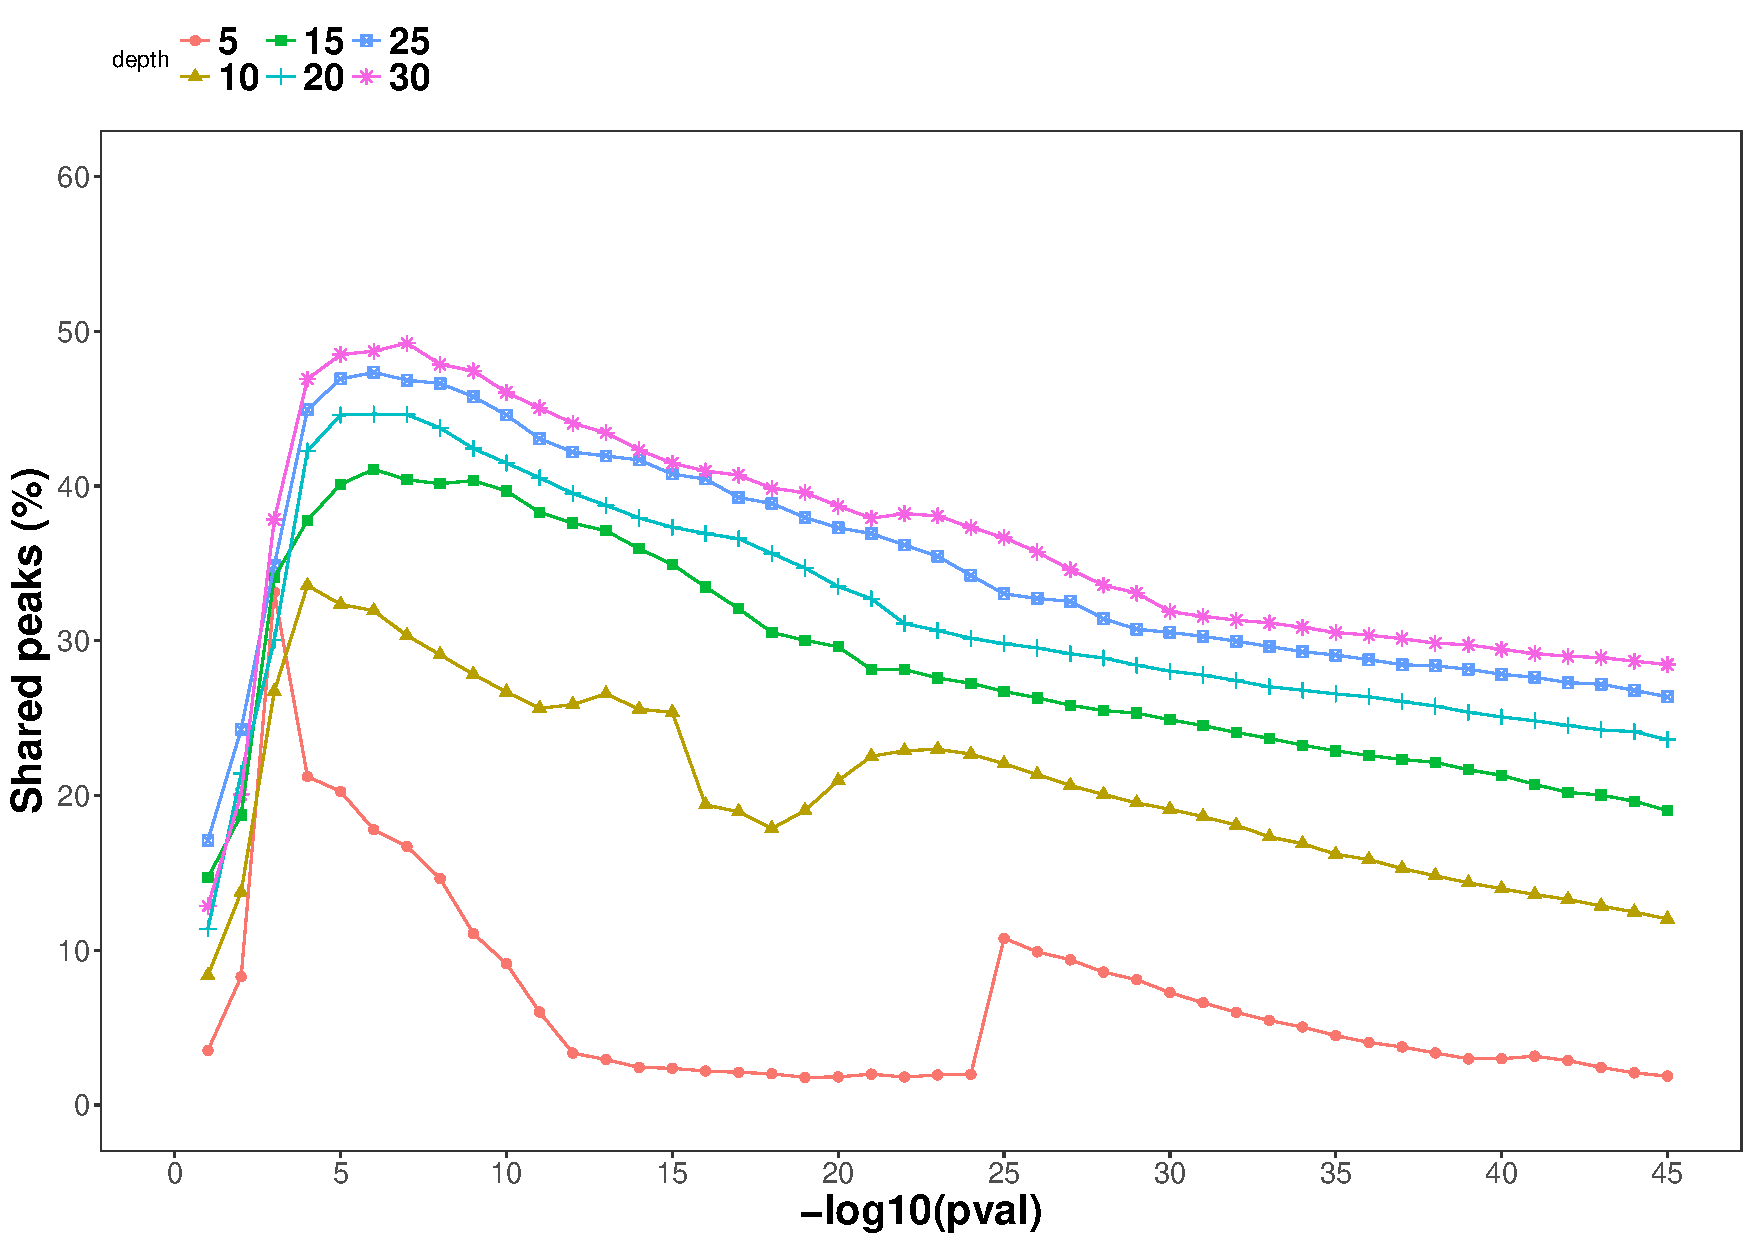
\includegraphics[width=\textwidth]{./Results1/pdfs/ATAC_Core_fresh_CTL2_CD14_shared_peaks_IDR_vs_pval}
\caption{\textbf{}}
\end{subfigure} \\
\begin{subfigure}{0.65\textwidth}
\centering
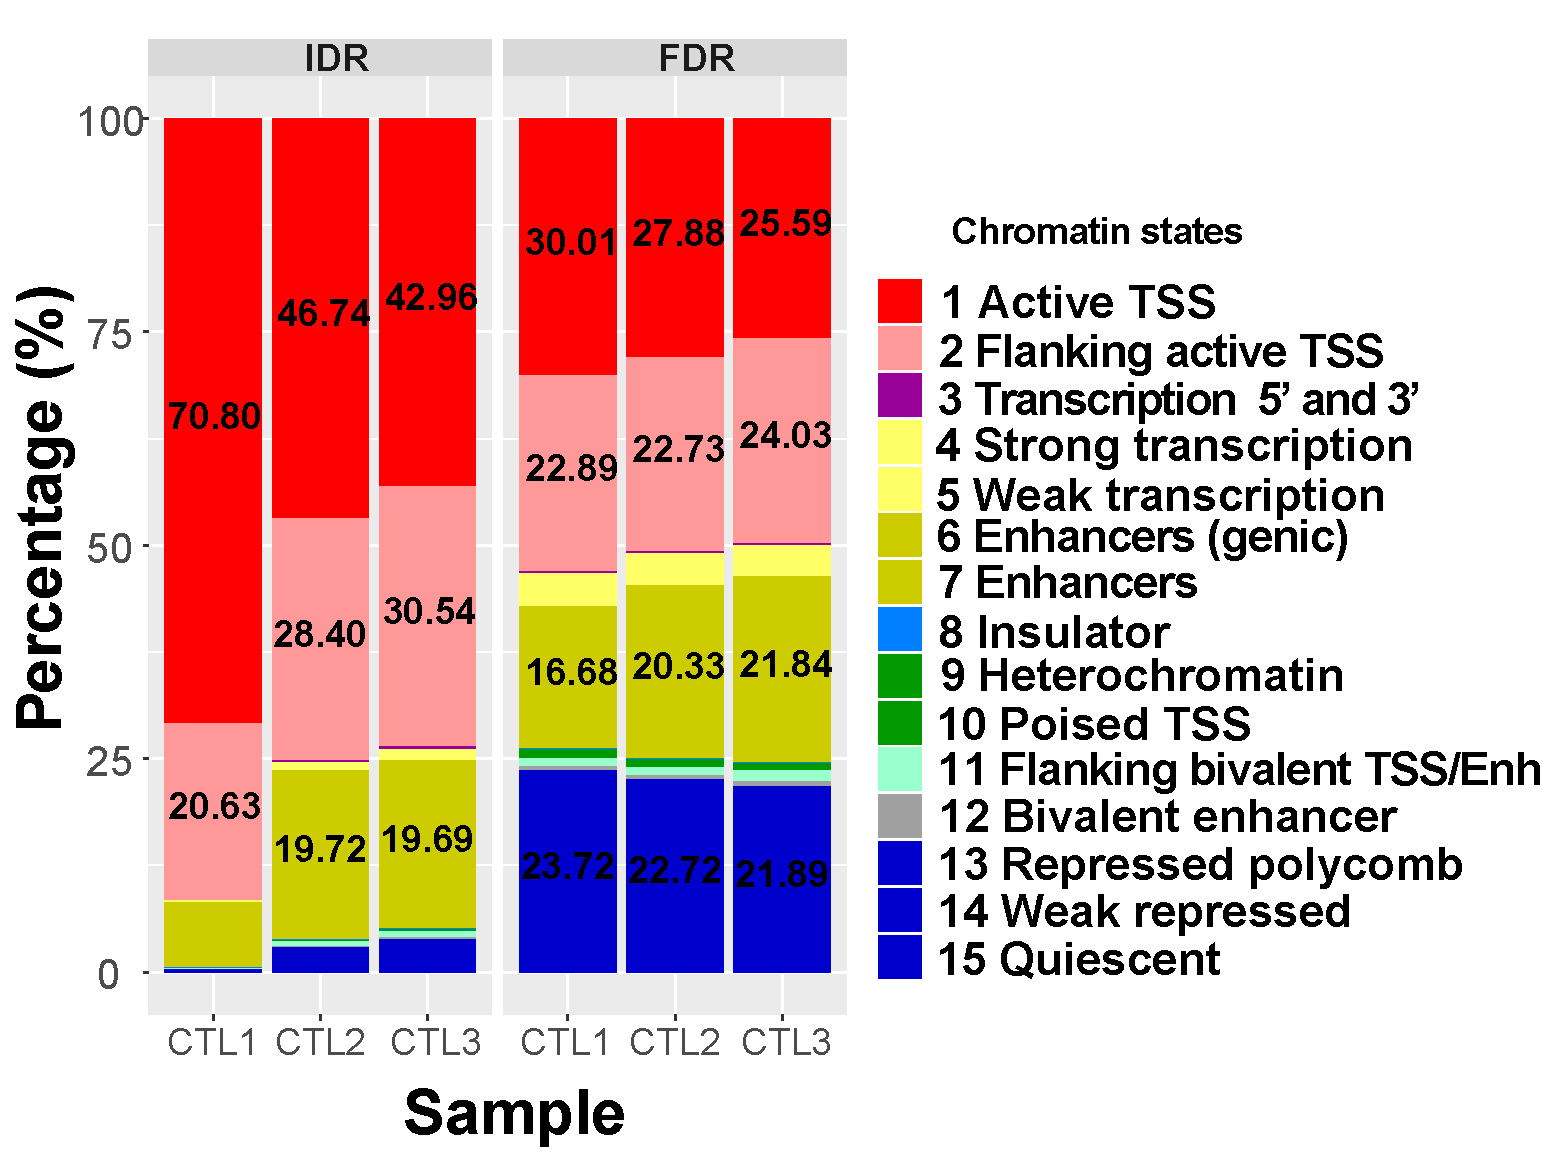
\includegraphics[width=\textwidth]{./Results1/pdfs/stacked_barplot_chromatin_states_percent_CD4_qval_vs_PVAL_IDR_filtered}
\caption{\textbf{}} % to add text to the figure name
\end{subfigure}%
\caption[Peak calling filtering using IDR analysis in ATAC-seq samples.]{\textbf{Peak calling filtering using IDR analysis in ATAC-seq samples.} For each of the sequencing depths tested (from 5 to 30 million reads after filtering), an illustration of the percentage of peaks sharing IDR rank between the two pseuroreplicates is shown when using different p-value filtering thresholds in CTL2 (A) CD14$^+$ monocytes and (B) CD4$^+$, two representative samples differing in quality for this analysis. (C) Annotation (as percentage of total) of the CTL1, CTL2 and CTL3 CD4$^+$ ATAC-seq peaks filtered for FDR$<$0.01 or optimal p-value from the IDR analysis (p-value=10$^{-11}$) with the corresponding cell type specific Roadmap Epigenomics Project chromatin segmentation map.}
\label{figure:Peak_calling_IDR_filtering_and_chrom_stated_ATAC}
\end{figure} 


Filtering the CD4$^+$ peaks at the p-value of the first local maximum (10$^{-11}$) reduced the percentage of peaks overlapping regions suggestive of noise (e.g repressed and quiescent), and increased the proportion of accessible regions located at active TSS when compared to using the list of significant peaks filtered based on FDR$<$0.01 (Figure \ref{figure:Peak_calling_IDR_filtering_and_chrom_stated_ATAC}C). In summary, this IDR analysis provided a systematic method to identify an optimum p-value with which to perform sample-specific filtering of technically reproducible peaks when the sequencing depth was over 10 million reads. These resulting filtered peaks will be used downstream to build the consensus list of ATAC peaks across all the samples and perform differential chromatin accessibility analysis. 

%Should mention that the median of all this first max are used to perform filtering for all the samples because following other pipelines they always use same filtering value for all samples so we need to be consistent across samples


\subsubsection{Differential chromatin accessibility analysis}

A peak-based approach using the number of reads overlapping the peaks included in the consensus list of ATAC peaks (CP\_all) was implemented to perform differential analysis. One of the main limitations of the ATAC-seq and Fast-ATAC protocols (discussed in Sections \ref{ATACseq} and \ref{Fast_ATAC}) is the background signal. Therefore, an empirical cut-off was identified to minimise the impact of background read counts on the peaks included for the differential analysis \parencite{Xinmin2005,Jonker2014}. Moreover, due to lack of consensus in terms of normalisation and differential analysis methods in ATAC-seq (as reviewed in Table \ref{tab:ATAC_comparative_methods}), two strategies were tested (Figure \ref{figure:ML_workflow}). The first involved quantile normalisation of the read count matrix and the use of limma voom to perform differential chromatin accessibility analysis. The second strategy used DESeq2 for both, normalisation and differential analysis.

The CP\_all matrix includes all peaks called significant (present) in at least 30\% of the six samples used in this section (Figure \ref{figure:ML_workflow} Step 1). This consensus list of ATAC peaks can include what may be considered background counts, i.e. reads overlapping regions not considered significant in a particular sample (absent) but called as significant (and threfore present) in other samples. The number of reads overlapping peaks in samples where that peak was not called significant (absent) were used to generate a density distribution plot of the background reads (Figures \ref{figure:ML_workflow} Step 2). From this plot, a sequence of twenty cut-offs was defined, with each value representing the number of counts shown by an increasing percentage of the total absent peaks (Figure \ref{figure:ATAC_absent_peaks_distribution}) and each cut-off was applied to filter out peaks from the CP\_all raw count matrix (not normalised) with values lower than the cut-off in more than three samples (Figure \ref{figure:ML_workflow} Step 3). A filter of three samples was chosen as it corresponds to the smallest number of biological replicates in this particular experimental design and ensures that peaks absent in one condition are retained. The resulting reduced matrix of low-noise peaks for each cut-off value was then normalised using quantile or DESeq2 (library size and variance stabilization Love \textit{et al.} 2014) and used to conduct differential analysis with limma voom or DESeq2 respectively. The results from this were used to determine an appropriate threshold for filtering background reads, as well as to compare the two analytical methods. 


\begin{landscape}
\begin{figure}[htbp]
\centering
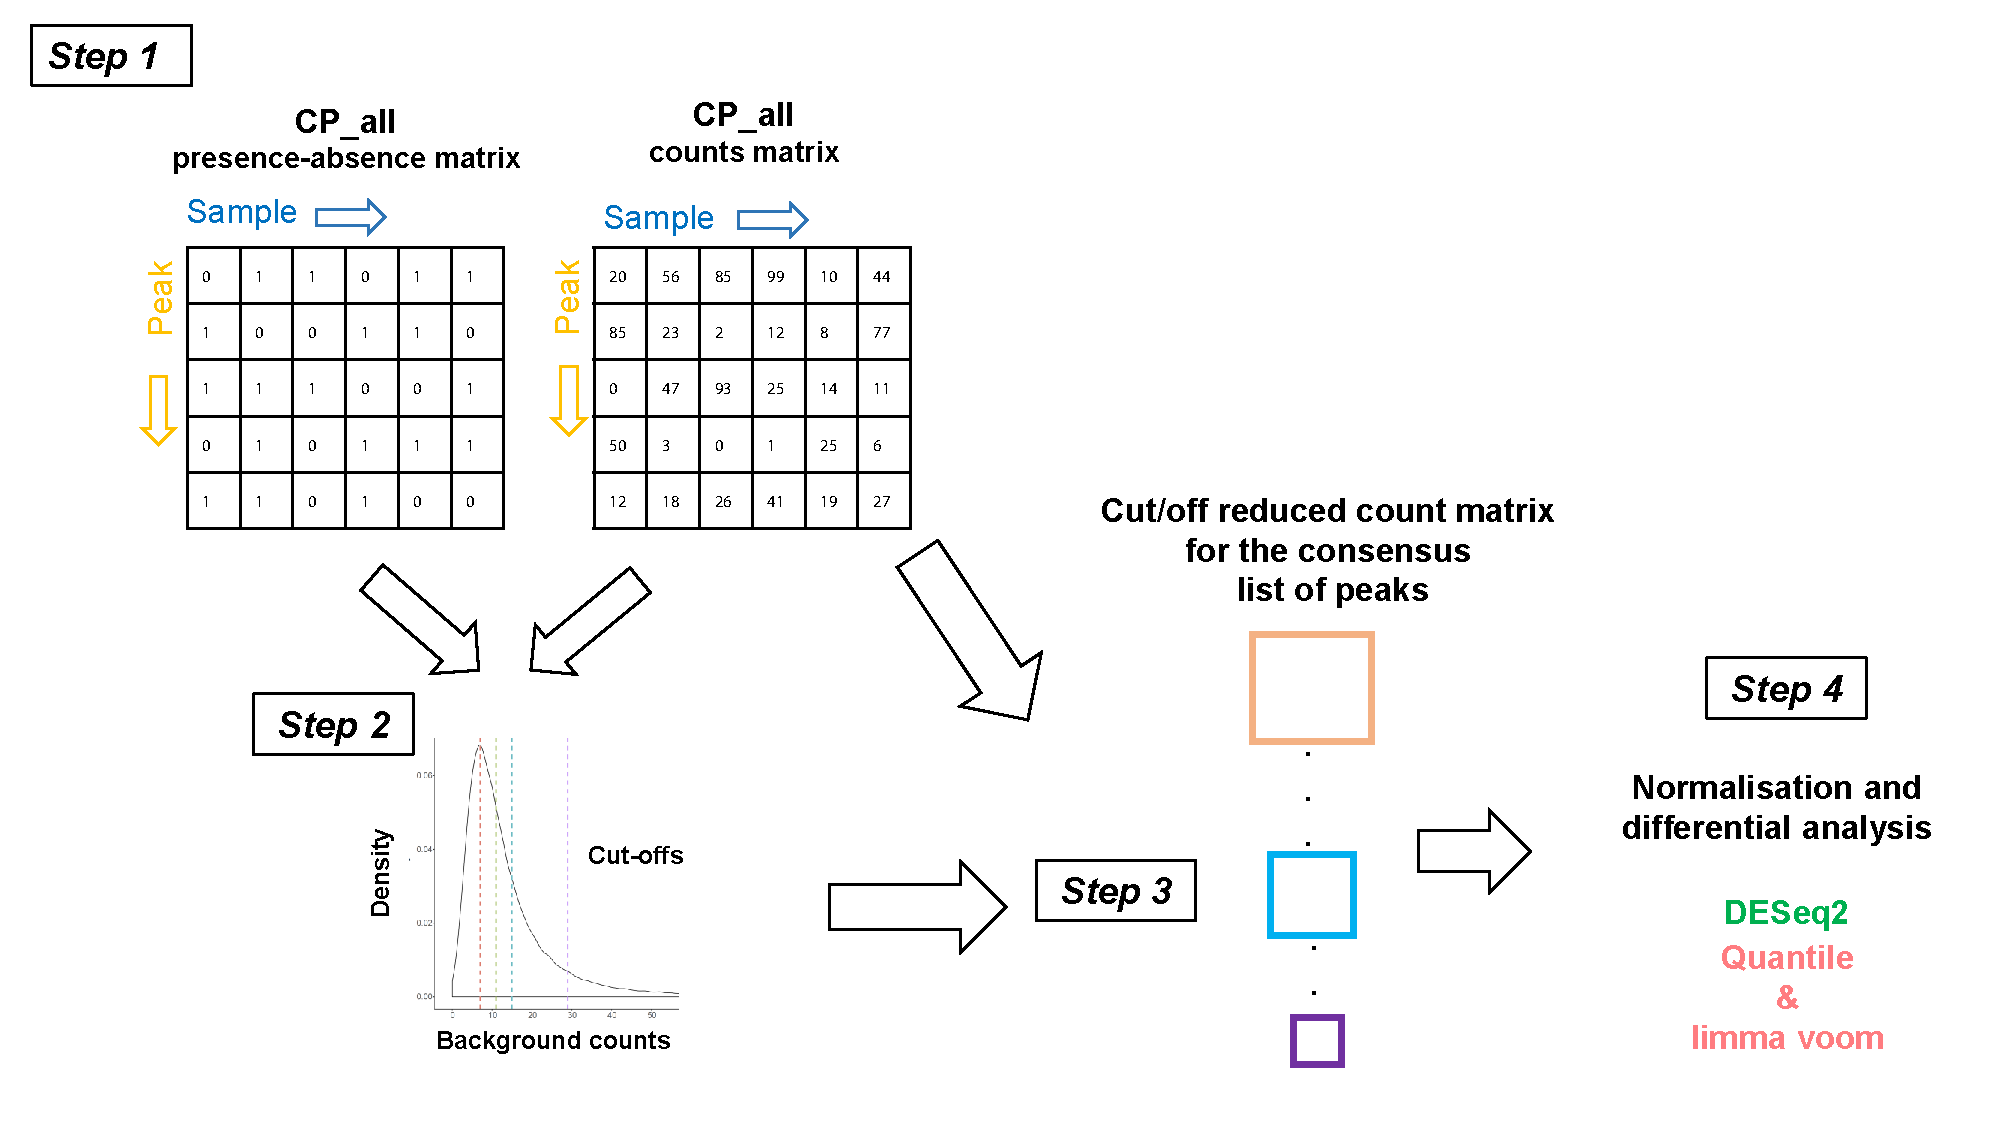
\includegraphics[width=1.2\textwidth]{./Results1/pdfs/ATAC_master_list_filtering_flow_chart}
\caption[Work flow illustrating the strategy to account for ATAC background noise prior to differential analysis.]{\textbf{Work flow illustrating the strategy to account for ATAC background noise prior to differential analysis.} A combined consensus list of ATAC peaks (CP\_all) was built as explained in Chapter \ref{ch:Mat}, including all the significant peaks that were shared by at least 30\% of the samples included in the analysis. The peaks were further transformed to obtain non-overlapping 500bp homogenous entities. The data was then represented by two matrices (Step 1). The first is the significance matrix with each cell indicating the significance of a peak (in rows) in each sample (in columns) as presence (1, significant) or absence (0, non-significant). The second matrix is the count matrix storing the number of reads mapped to the peak (in rows) for each sample (in columns). A density distribution plot of the read counts from the peaks absent (0) in each sample was used to define a sequence of twenty cut-offs. These cut-offs correspond to the number of counts showed by a particular percentage of the absent peaks and can be considered background counts (Step 2). The defined cut-offs were used to filter out peaks from the CP\_all and generate a series of reduced matrices (Step 3) that were tested for normalisation and differential chromatin accessibility analysis by two methods (quantile \& limma voom or DESeq2) (Step 4).}
\label{figure:ML_workflow}
\end{figure}
\end{landscape}



%\ToDo{From the count matrix for the six samples defined above, the read counts from those peaks that were absent in each sample (since the  CP\_all includes peaks present in at least 30\% of the total samples)(Figure \ref{figure:ML_workflow} Step 1) were used to generate a density distribution plot (Figure \ref{figure:ML_workflow} Step 2). From this plot, a sequence of twenty cut-offs were defined, with each representing the number of counts showed by a particular percentage of the total absent peaks (Figure \ref{figure:ATAC_absent_peaks_distribution}). Each cut-off was used to filter out peaks from the CP\_all raw count matrix (without normalisation) whose values in more than three samples were lower than the background counts (Figure \ref{figure:ATAC_absent_peaks_distribution} Step 3). A filter of three samples were chosen, as it corresponds to the smallest group of replicates in this particular experimental design and ensures peaks absent in one condition were retained. As a result, each cut-off generates a reduced matrix of low-noise peaks that was normalised using quantile or DESeq2 (library size and variance stabilisation \parencite{Love2014}) and used to conduct differential analysis with limma voom or DESeq2, respectively. Both normalisation methods performed appropriately for all the reduced consensus list of ATAC peaks across the six samples, with slightly greater consistency for the quantile normalisation across the two groups (Figure \ref{figure:ATAC_normalisation_and_DARs_limma_DESeq2}A and B). Differential chromatin accessibility analysis using quantile normalisation counts \& limma voom showed a greater number of significant (FDR$<$0.01 and fold change$>$1.5) differentially accessible regions (DARs) compared to DESeq2, across all filtering cut-offs (Figure \ref{figure:DOC_quantile_DESeq2}C). The two approaches presented a progressive decrease in the number of DARs from the 75\% cut-off onward, suggesting a reduction in the number of false positive hits reported for peaks with read counts close to the background noise cut-off. Further increases in the cut-off value however are expected to also remove true positives, so an intermediate value is chosen here. Depending on the noise inherent to an experiment this threshold may vary.} 


Both normalisation methods performed appropriately across all filter values and samples, with the quantile normalisation showing slightly greater consistency across the two groups (Figure \ref{figure:ATAC_normalisation_and_DARs_limma_DESeq2}A and B). Differential chromatin accessibility analysis using limma voom showed a greater number of significant (FDR$<$0.01 and fold change$>$1.5) differentially accessible regions (DARs) compared to DESeq2 across all filtering cut-offs. For both approaches, the number of DARS progressively decreased as the filtering cut-off increased from 75\% onwards (Figure \ref{figure:ATAC_normalisation_and_DARs_limma_DESeq2}C).




\begin{figure}[ht]
\centering
\begin{subfigure}{0.45\textwidth}
\centering
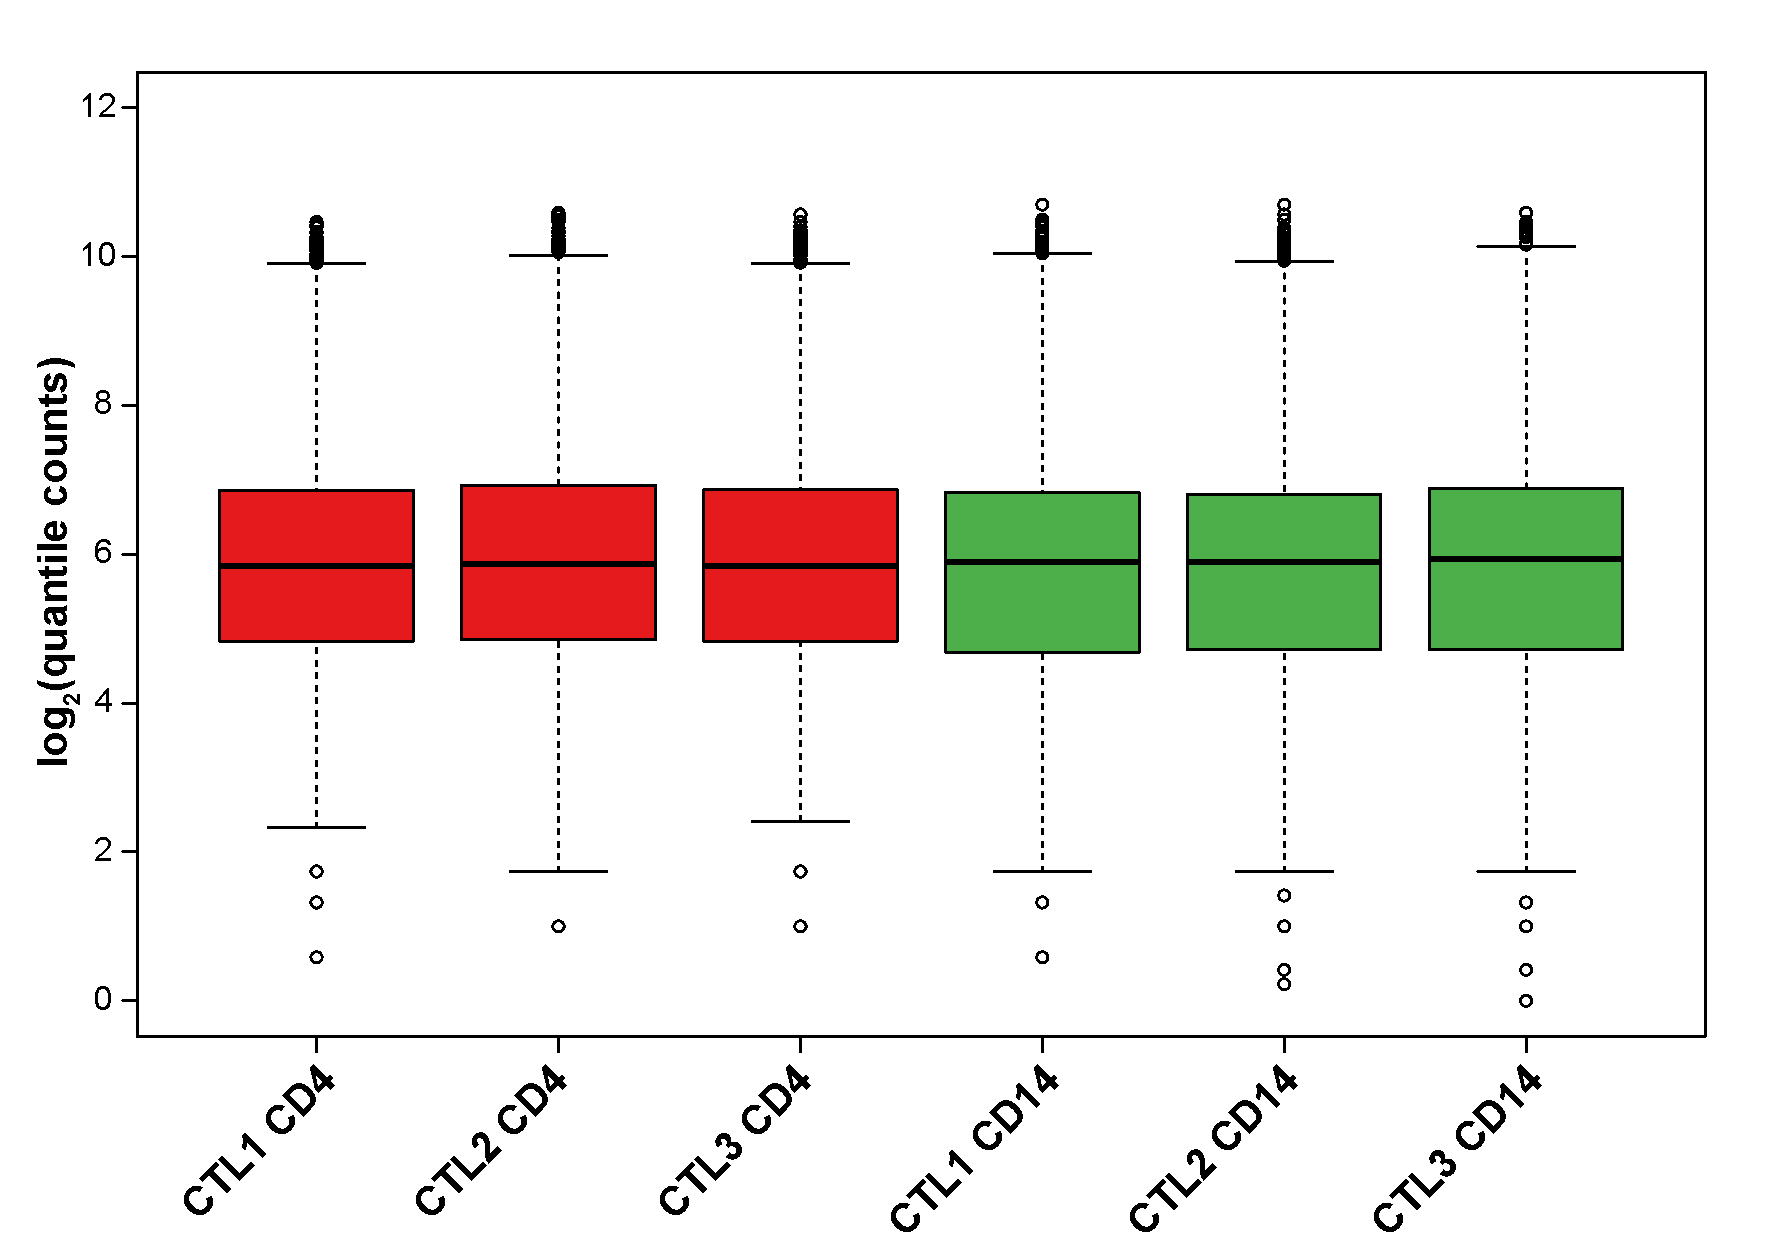
\includegraphics[width=\textwidth]{./Results1/pdfs/ATAC_Core_CD4_CD14_boxplot_80pcnt_cut_off_filtered_quantile_counts}
\caption{\textbf{}}
\end{subfigure}%
\begin{subfigure}{0.45\textwidth}
\centering
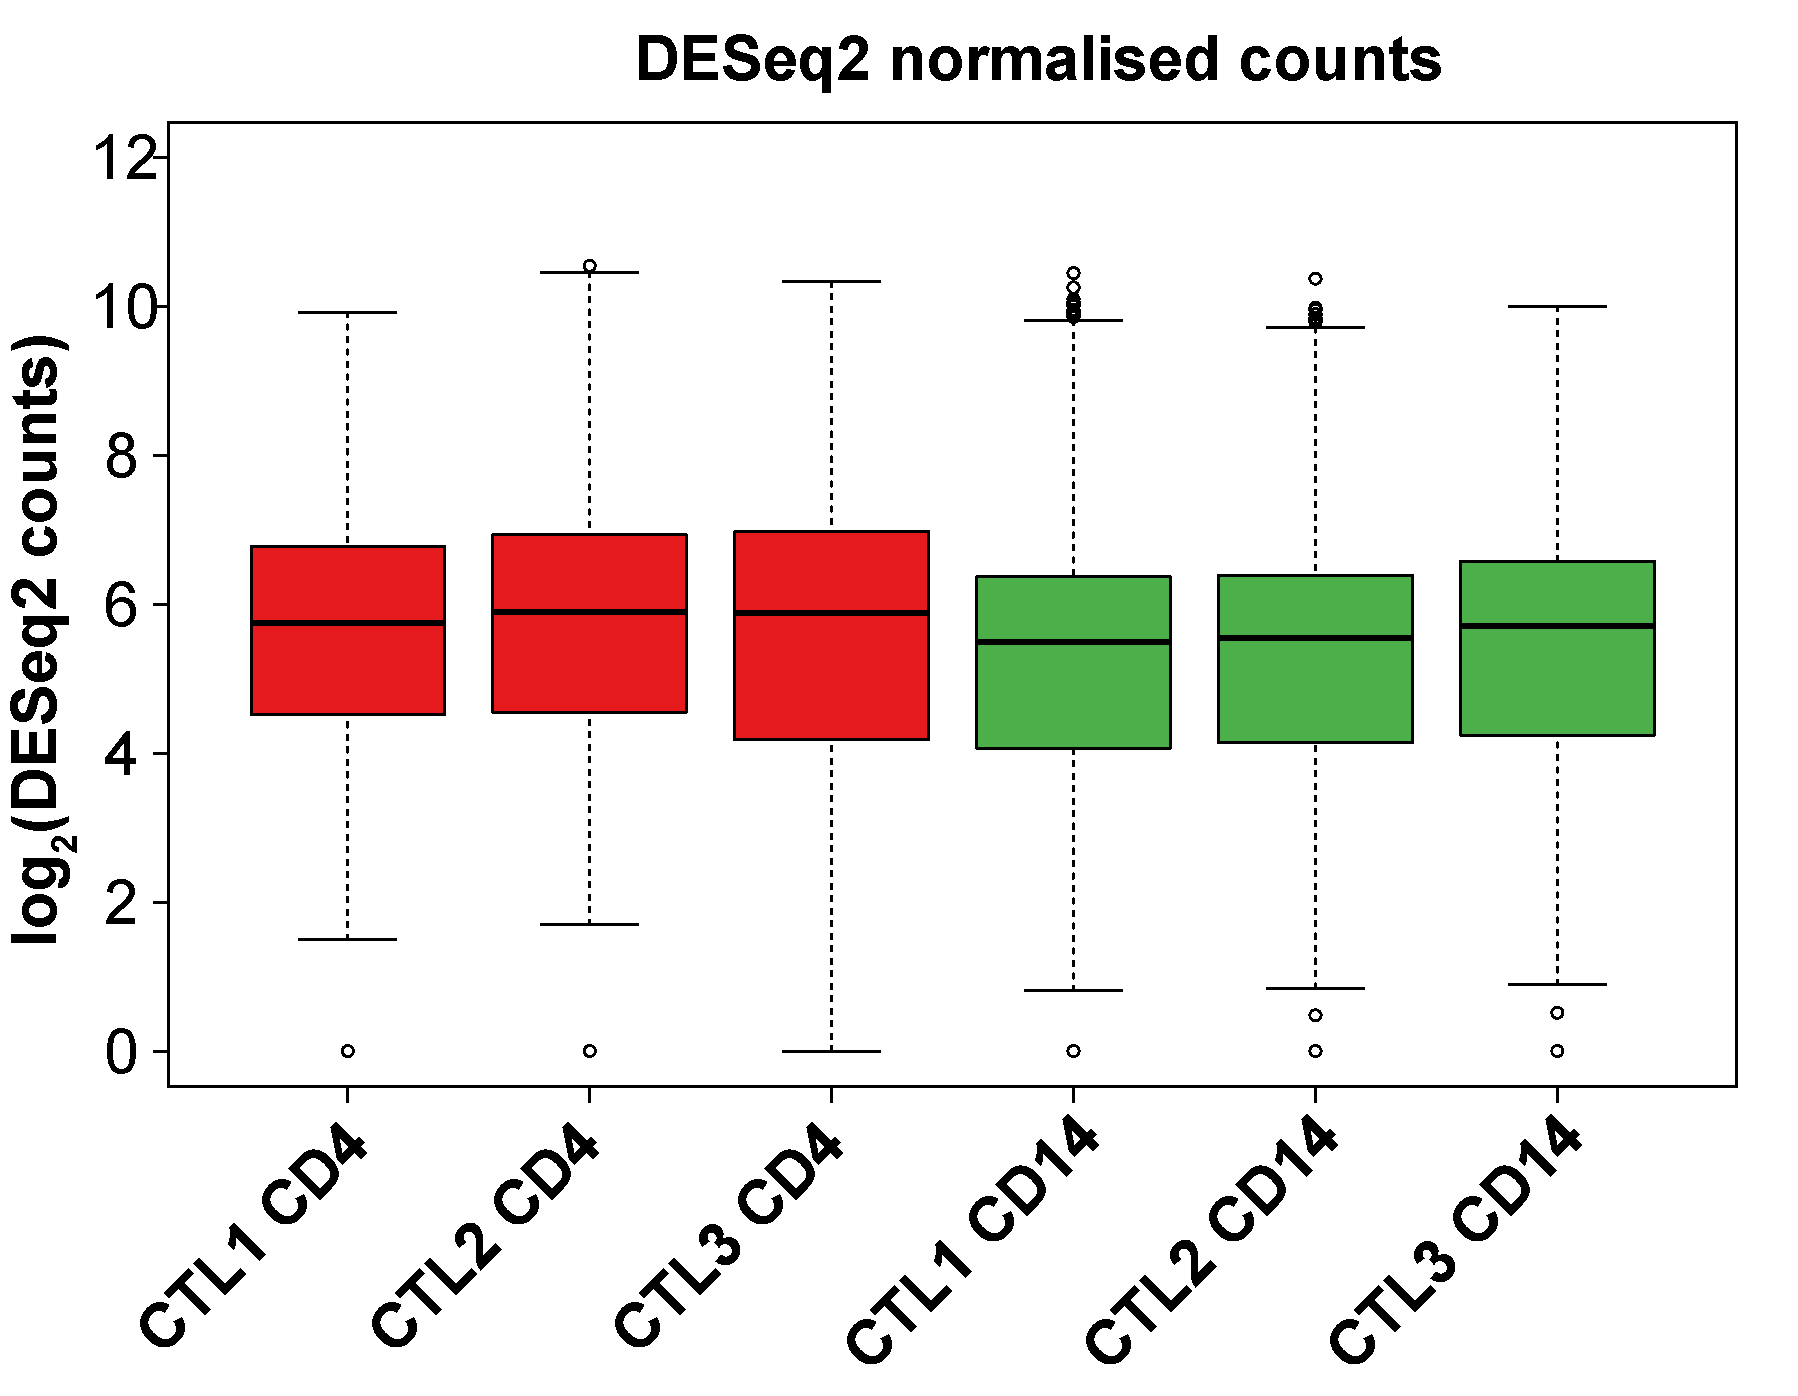
\includegraphics[width=\textwidth]{./Results1/pdfs/ATAC_Core_fastq_CD4_CD14_DESeq2_mean_vs_log2sd}
\caption{\textbf{}}
\end{subfigure}
\begin{subfigure}{0.5\textwidth}
\centering
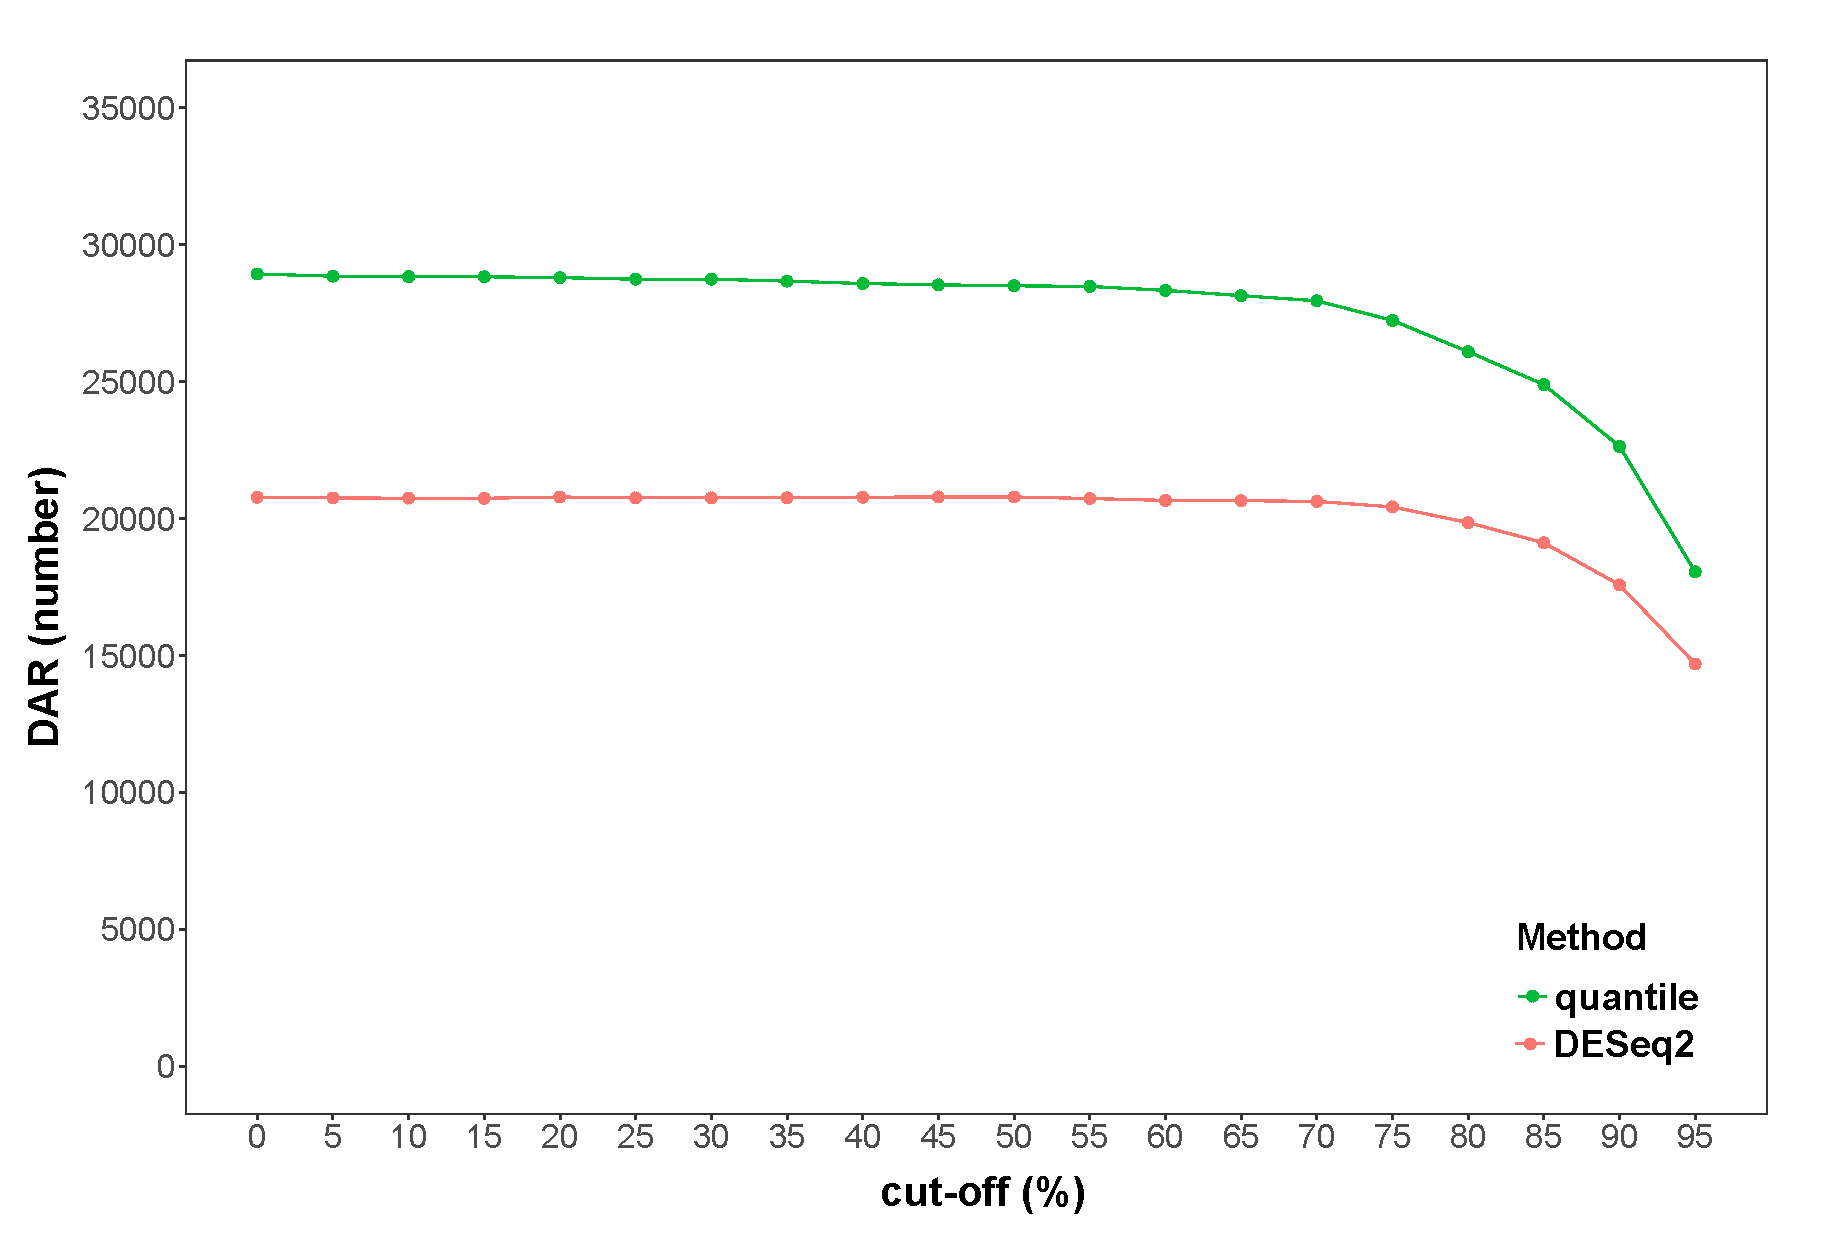
\includegraphics[width=\textwidth]{./Results1/pdfs/ATAC_Core_CD4vsCD14_DOC_FDR_01_vs_cutoffs_quantile_DESeq2_only}
\caption{\textbf{}}
\end{subfigure}

\caption[Normalisation and differential chromatin accessibility analysis for different cut-offs using quantile normalisation limma voom and DESeq2.]{\textbf{Normalisation and differential chromatin accessibility analysis for different cut-offs using quantile normalisation\& limma voom and DESeq2.} Boxplots representing the log$_2$  read counts for each of the peaks from the unfiltered consensus list of peaks normalised by (A) quantile or (B) DESeq2 in the three CD14$^+$ monocytes and total CD4$^+$  healthy control paired samples. (C) Representation of the number of significant DARs (FDR$<$0.01 and FC$>$1.5) detected in the differential analysis by limma voom (using quantile normalisation) or DESeq2 when using a sequence of empirical background noise cut-offs to filter the consensus list of peaks.}
\label{figure:ATAC_normalisation_and_DARs_limma_DESeq2}
\end{figure} 

This suggested a reduction in the number of false positive hits resulting from peaks with high background reads. However, increasingly stringent filtering would also remove true positives so an intermediate value of 80\% was chosen here. In future analyses this value may vary depending on the noise inherent to the experiment.



\begin{figure}[htbp]
\centering
\begin{subfigure}{0.5\textwidth}
\centering
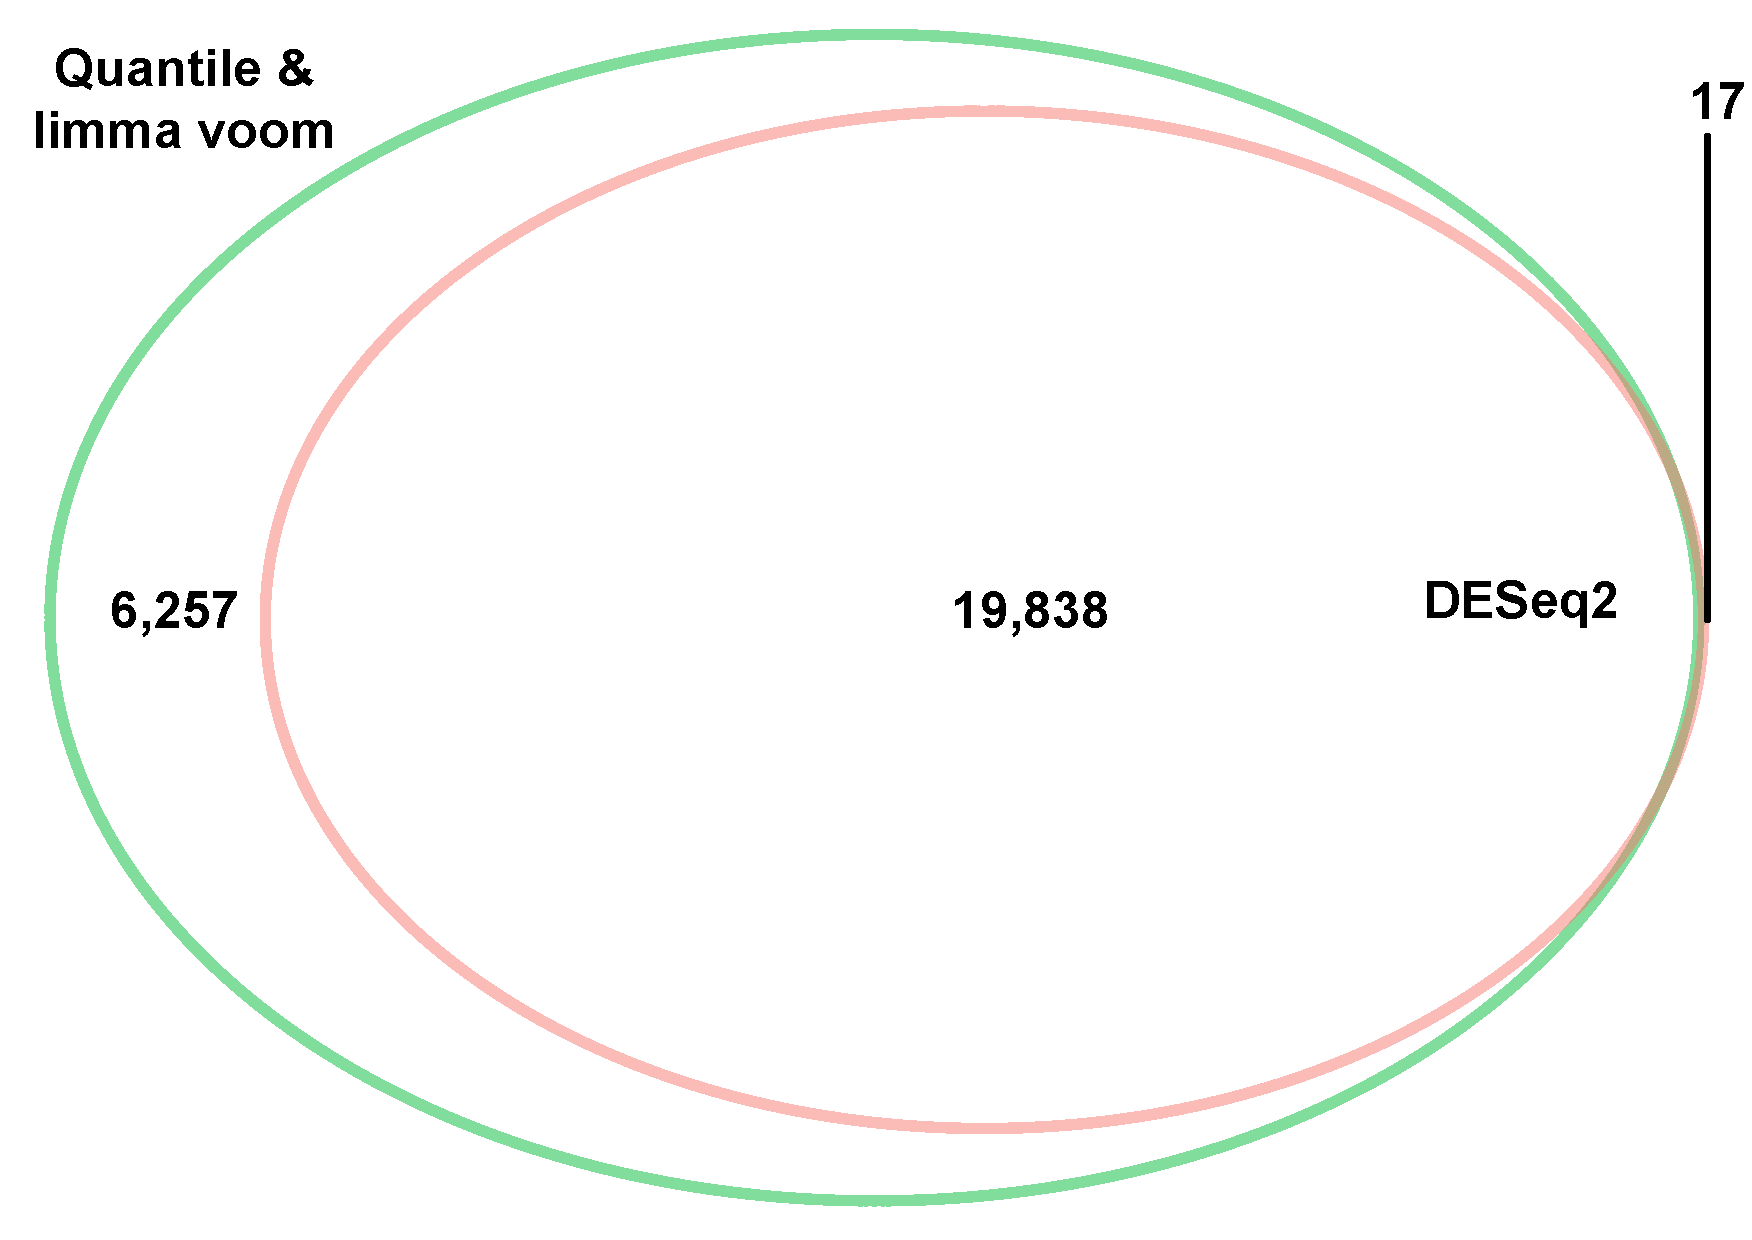
\includegraphics[width=\textwidth]{./Results1/pdfs/ATAC_Core_fresh_CD4vsCD14_venn_diagram_differential_analysis_FDR_01_quantile_DESeq2_only}
\caption{\textbf{}}
\end{subfigure}
\begin{subfigure}{0.5\textwidth}
\centering
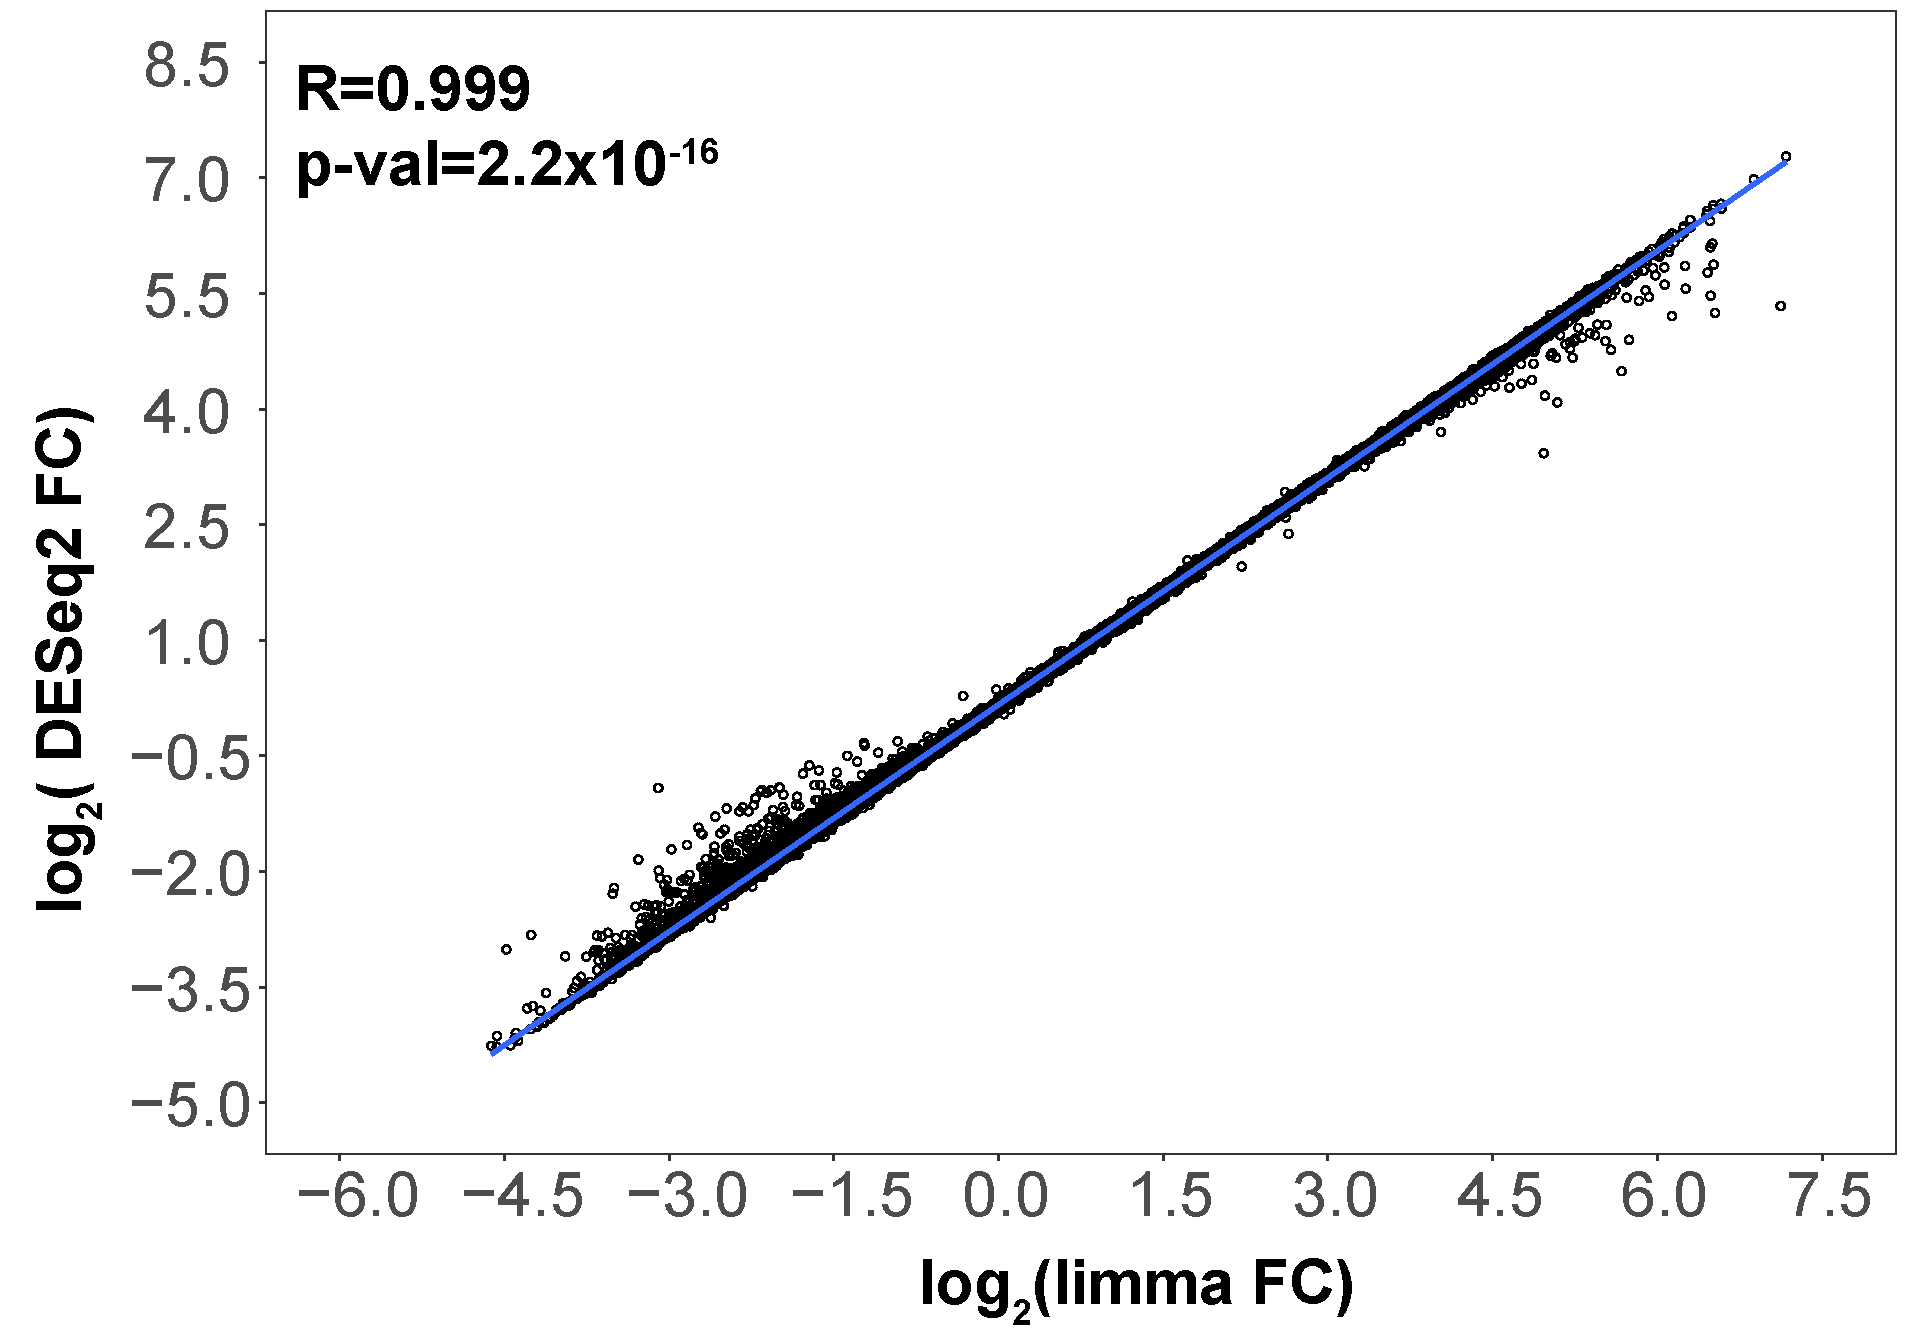
\includegraphics[width=\textwidth]{./Results1/pdfs/ATAC_Core_fastq_CD4_CD14_80pcnt_cut_off_correlation_log2FC_quantile_vs_deseq2}
\caption{\textbf{}} % to add text to the figure name
\end{subfigure}
\caption[Comparison of the DARs identified by differential analysis using limma voom or DESeq for the consensus peak list filtered at the optimal cut-off 80\%.]{\textbf{Comparison of the DARs identified by differential analysis using limma voom or DESeq for the consensus peak list filtered at the optimal cut-off 80\%.} (A) Venn diagram illustrating the common and distinct significant (FDR$<$0.01 and fold change$>$1.5) DARs identified by differential analysis in the filtered consenus list of ATAC peaksfor the 80\% optimal cut-off using limma voom or DESeq2. (B) Representation of the correlation between limma voom and DESeq2 log$_2$ fold changes (no FDR filtered) in each the peaks from the fconsensus list of peaks filtered at the 80\% optimal cut-off. Pearson correlation coefficient (R) and significance (p-value) are indicated. Limma voom was applied to quantile normalised count data.}
\label{figure:QC_quantile_DAR_and_DESeq2_comparison}
\end{figure} 


The vast majority of the 19,855  DARs called as significant using the more conservative method (DESeq2) were recapitulated by limma voom at the same significance threshold (FDR$<$0.01 and fold change$>$1.5) (Figure \ref{figure:QC_quantile_DAR_and_DESeq2_comparison}A). FDR rank revealed that out of the first 19,855 limma voom DARs 18,768 matched the rank of those retrieved by DESeq2. Moreover, very significant positive correlation was found between fold changes for all the regions included in the 80\% cut-off reduced matrix reported by the two methods (R=0.999, p-value=2.2$^{-16}$) (Figure \ref{figure:QC_quantile_DAR_and_DESeq2_comparison}B). Overall, this suggested that the differences in the number of significant DARs reported by limma voom and DESeq2 could partly be driven by differences in the models used by the two methods to estimate dispersion of counts. 

Lastly, the significant  DARs identified by DESeq2 and filtered for FDR$<$0.01 and fold change$>$1.5 were divided in those more accessible in CD14$^+$ monocytes  (open in monocytes) or CD4$^+$ (open in CD4$^+$). Enrichment analysis for cell type-specific epigenetic features, including FANTOM5 eRNAs, histone marks and DHSs, was conducted in each of the two groups of DARs. The CD4$^+$ open DARs were enriched for T cell eRNAs, CD4$^+$ H3Kme1 and H3K27ac and CD14$^+$ DHSs (Figure \ref{figure:Enrichment_analysis_of_DARs_by_DESeq2}). Conversely, the top enriched features for CD14$^+$ monocytes open DARs included eRNAs, H3K27ac and DHSs in monocytes. Overall, this enrichment analysis confirmed the ability of this differential analysis method to identify significant and robust DARs that highlight cell-type specific regulatory regions for CD14$^+$ monocytes and CD4$^+$ cells.

\begin{figure}[h]
\centering
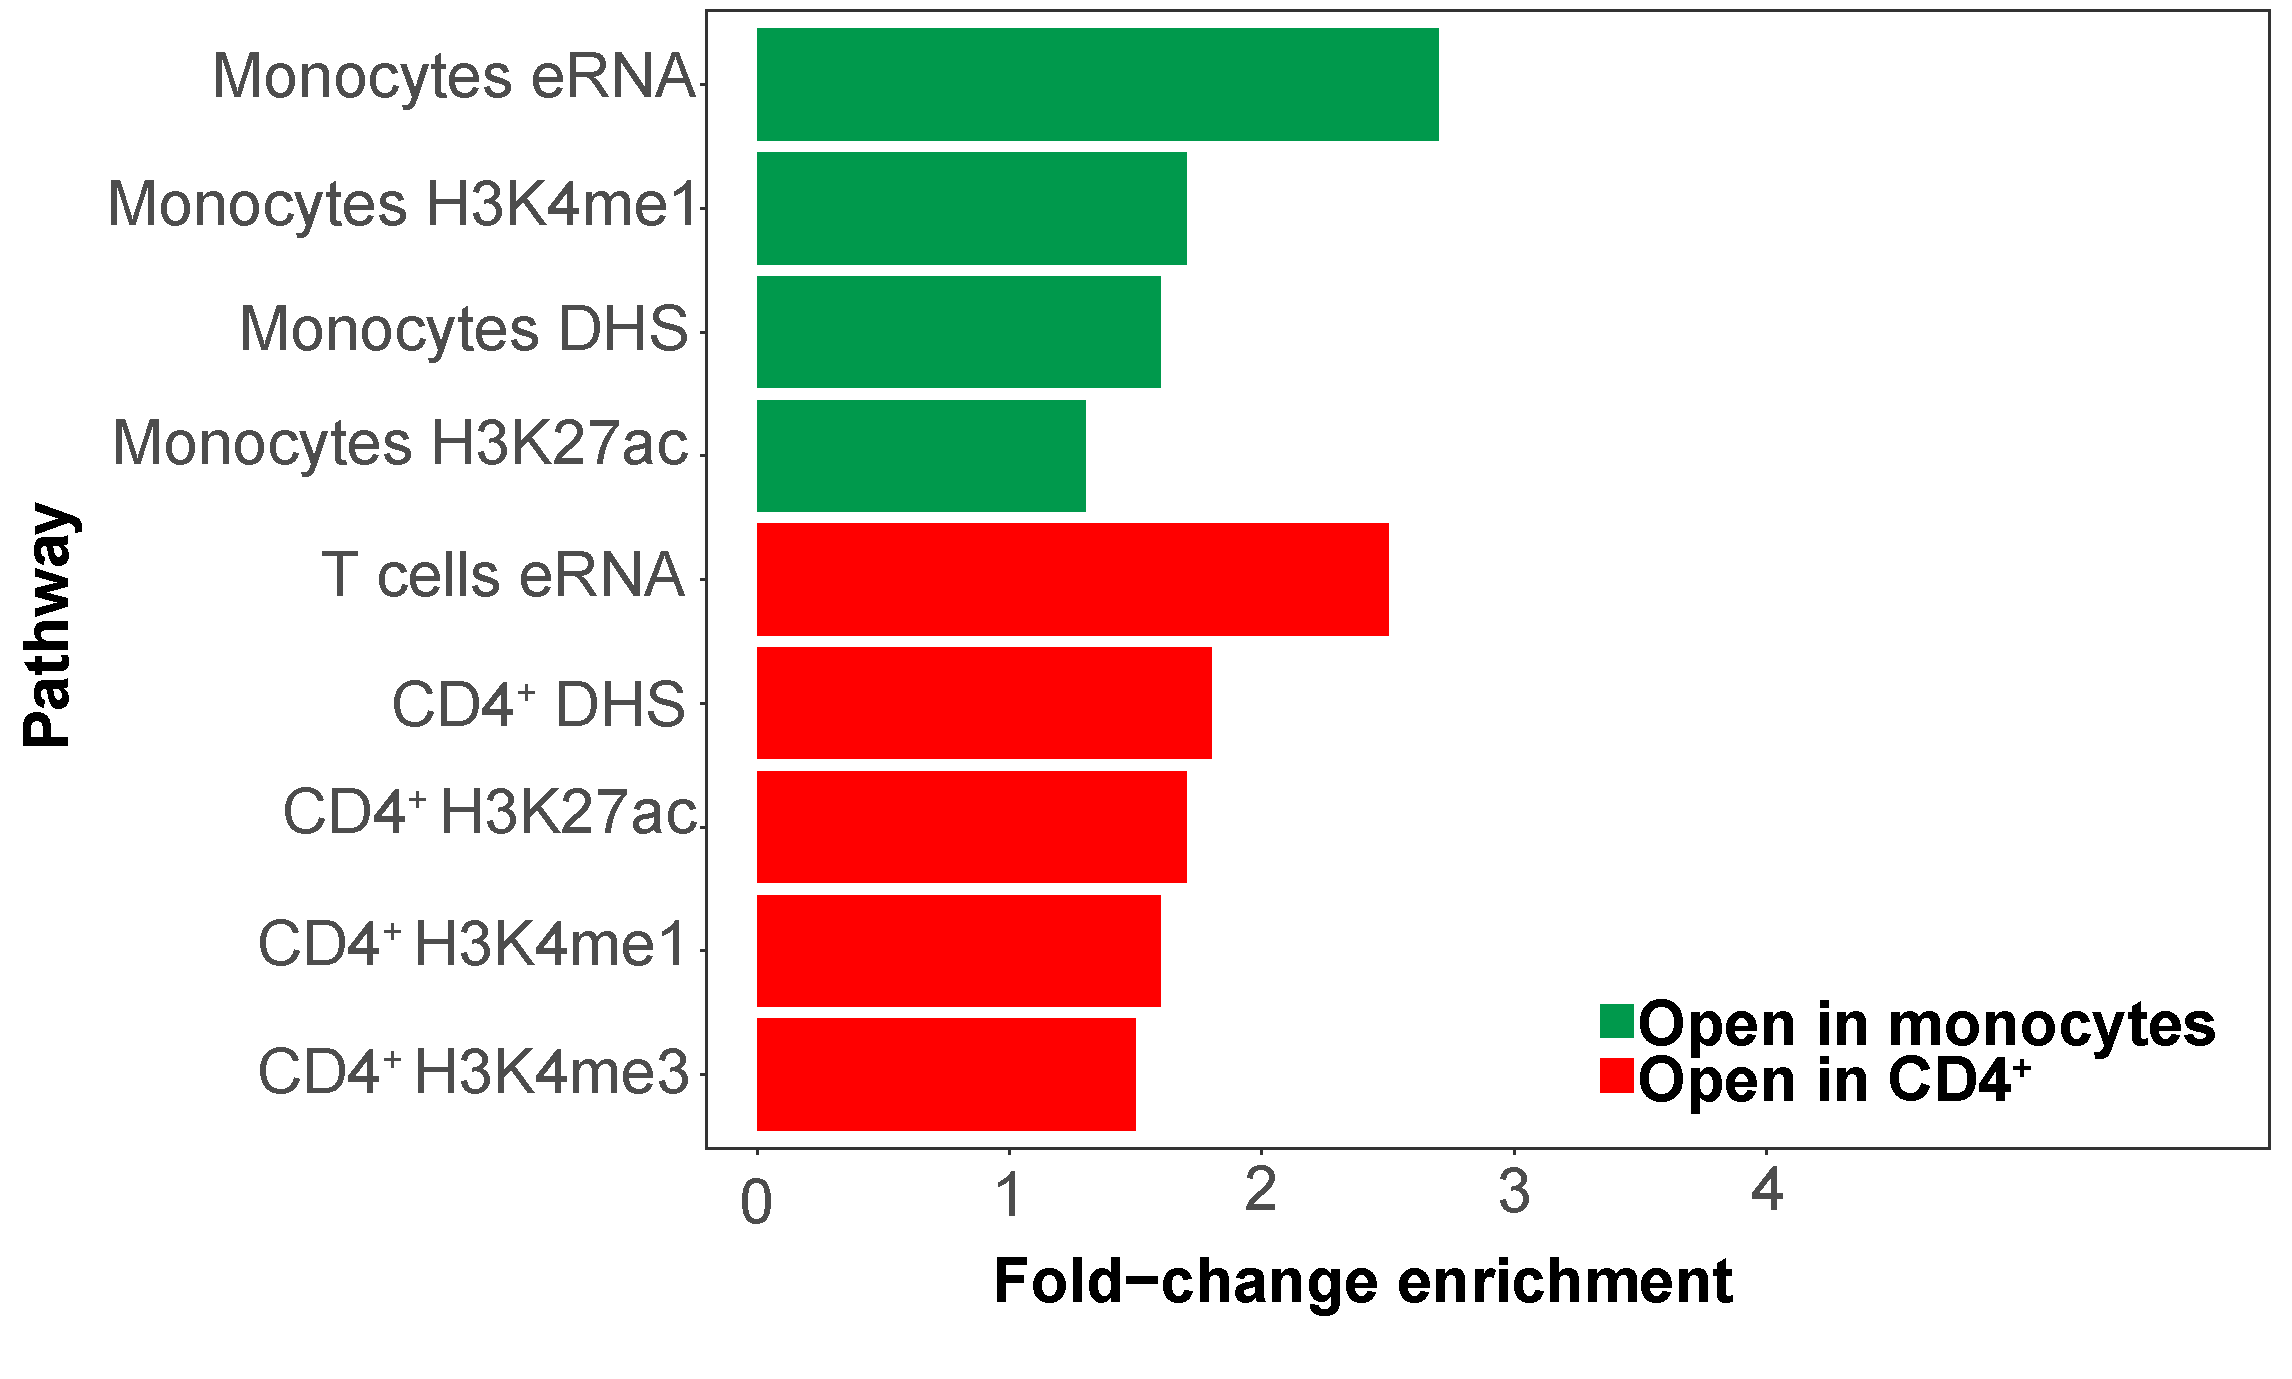
\includegraphics[width=0.6\textwidth]{./Results1/pdfs/ATAC_CD4vsCD14_deseq_features_enrichment_barplot}
\caption[Enrichment analysis for the significant DARs identified by DESeq2 between CD14$^+$ monocytes and CD4$^+$ cells.]{\textbf{Enrichment analysis for the for the significant DARs identified by DESeq2 between CD14$^+$ monocytes and CD4$^+$ cells.} Barplot representing the fold change for the top significantly enriched (FDR$<$0.01) FANTOM5 eRNAs and, histone marks and DHSs from Blueprint. Enrichment analysis was performed separately for the significant (FDR$<$0.01 and fold change$>$1.5) DARs more accessible in CD14$^+$ monocytes (open in monocytes) or CD4$^+$ (open in CD4$^+$).}
\label{figure:Enrichment_analysis_of_DARs_by_DESeq2}
\end{figure} 



%\begin{figure}[htbp]
%\centering
%\begin{subfigure}{0.65\textwidth}
%\centering
%\includegraphics[width=\textwidth]{./Results1/pdfs/ATAC_Core_CD4vsCD14_clusters_and_heatmap_DESeq2_only}
%\caption{\textbf{}}
%\end{subfigure}
%\begin{subfigure}{0.5\textwidth}
%\centering
%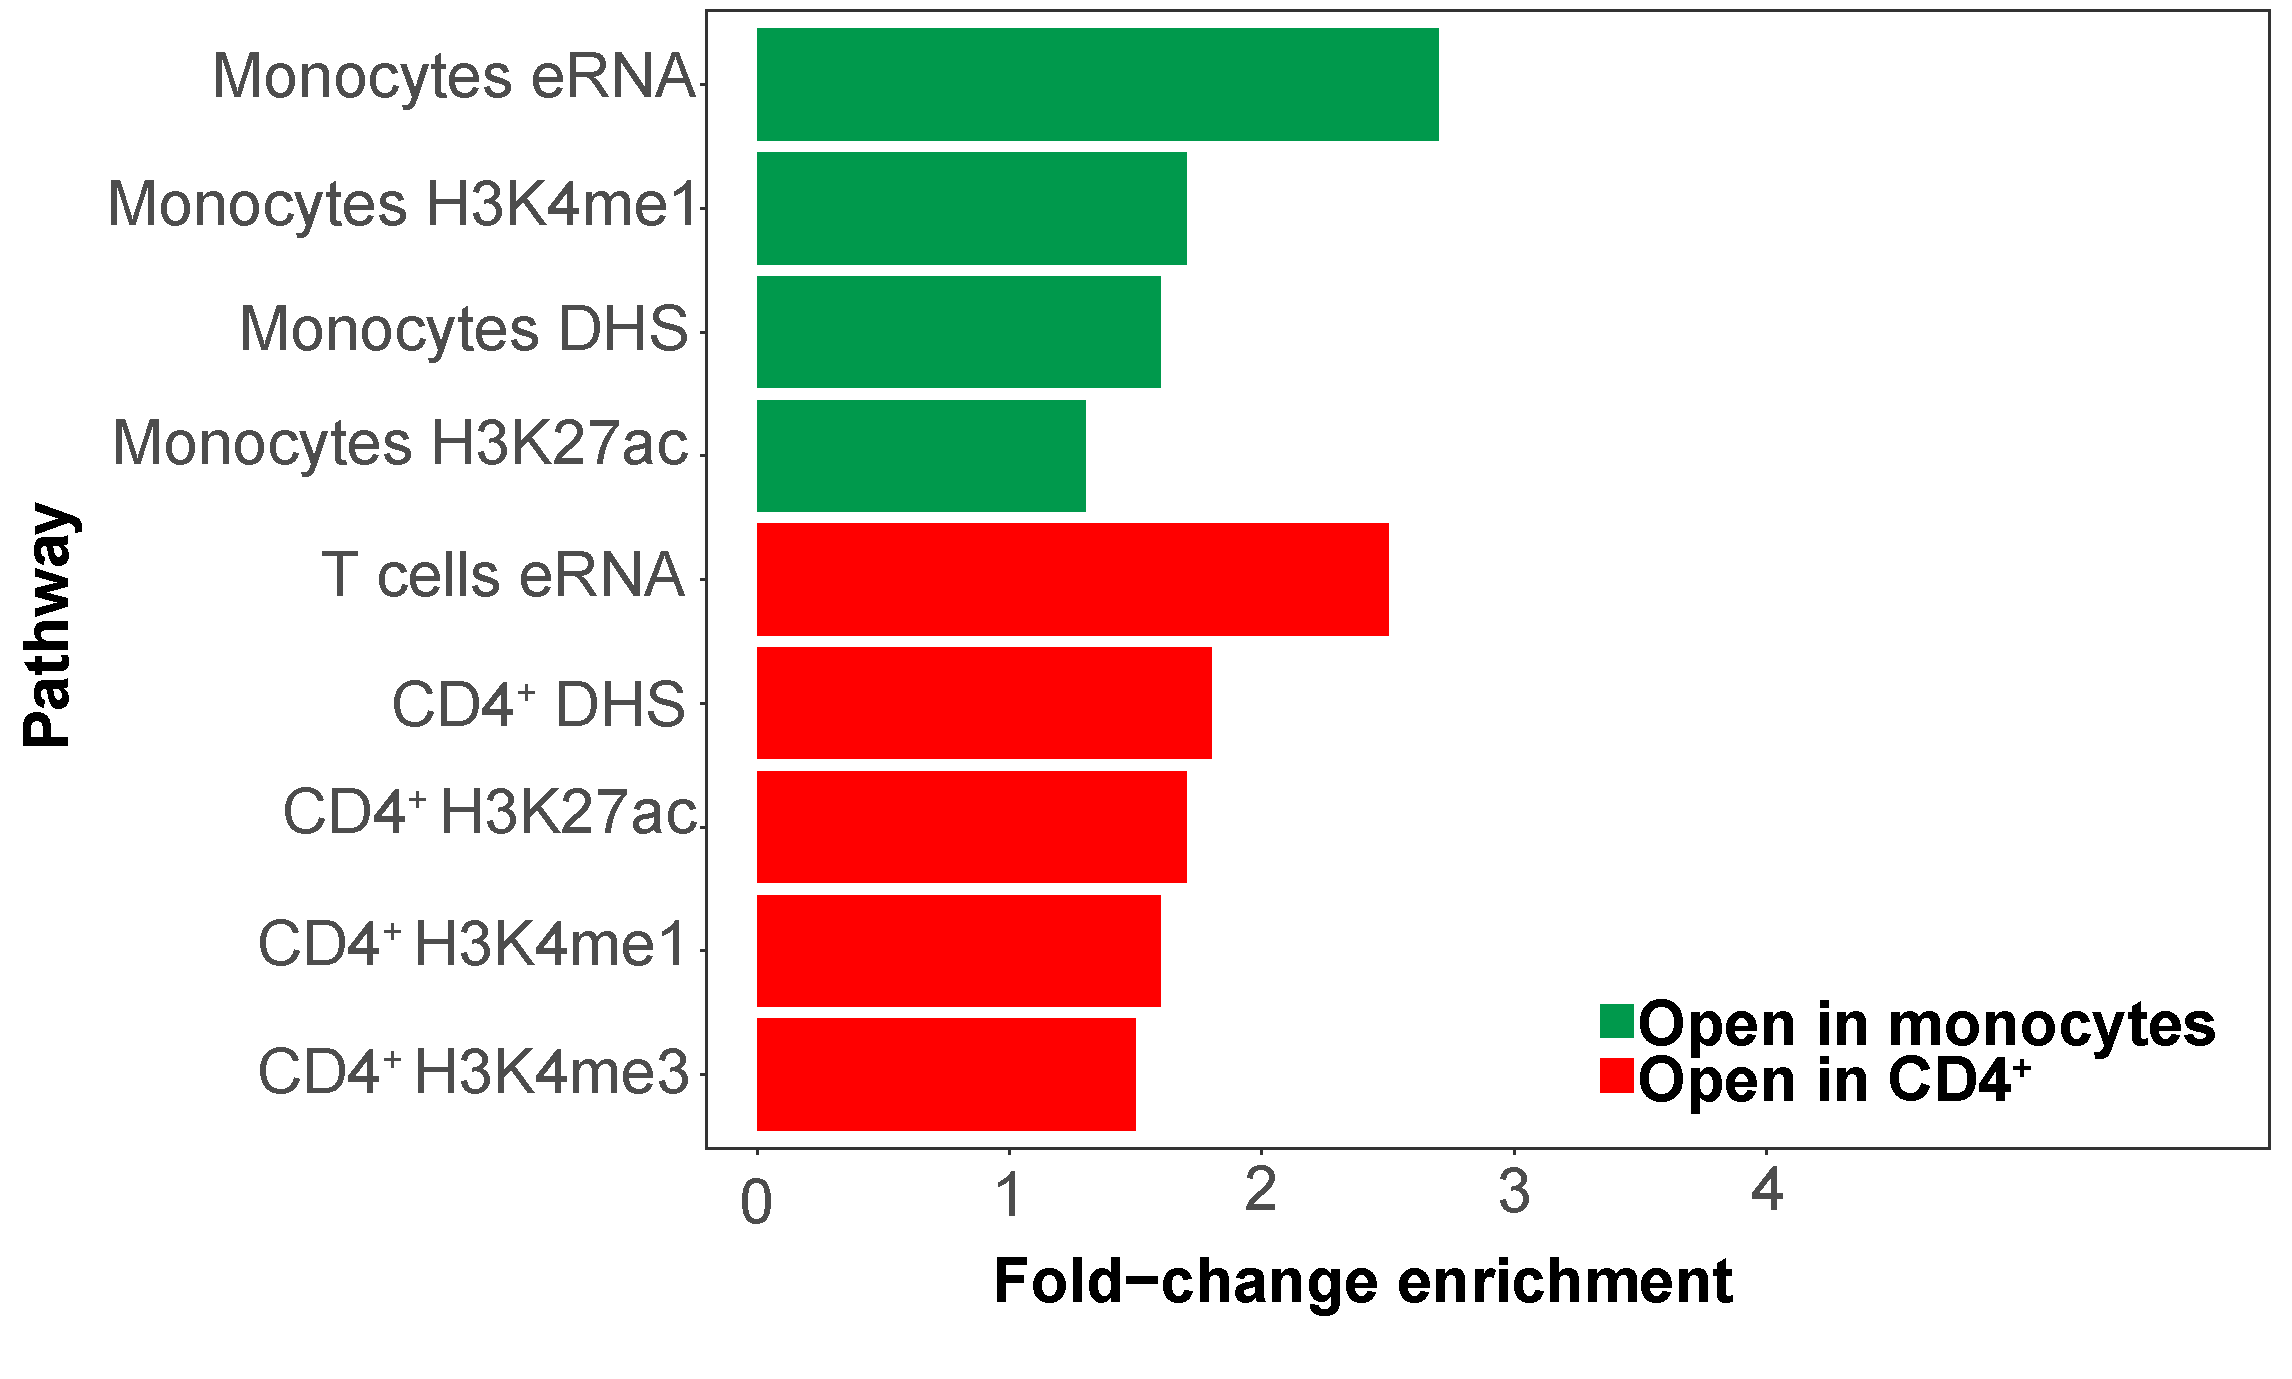
\includegraphics[width=\textwidth]{./Results1/pdfs/ATAC_CD4vsCD14_deseq_features_enrichment_barplot}
%\caption{\textbf{}} % to add text to the figure name
%\end{subfigure}
%\caption[Clustering heatmap and enrichment analysis for the significant DARs identified by DESeq2 between CD14$^+$ monocytes and CD4$^+$ cells.]{\textbf{Clustering heatmap and enrichment analysis for the identified DARs by DESeq2 between CD14$^+$ monocytes and CD4$^+$ cells.} (A)Heatmap showing for each of the ATAC-seq samples included in this analysis, the log$_2$ normalised counts at each of the 19,838 significant (FDR$<$0.01 and abs(fold change)$>$1.5) DARs identified by DESeq2. Each row represents a DAR and are clustered based on DARs presenting similar patterns of accessibility in each of the three replicates for the two cell types compared. (B) Barplot representing the fold change for the top significantly enriched (FDR$<$0.01) FANTOM5 eRNAs and Blueprint histone marks and DHSs.}
%\label{figure:Heatmap_and_enrichment_analysis_of_DARs_by_DESeq2}
%\end{figure} 
%

\bigskip %bigger space



\subsection{Assessment of ATAC-seq transposition times in relevant cell types}
\label{ATACseq}

The duration of the transposition reaction was optimised for the main immune cell types of interest for this thesis. ATAC-seq was performed for three different transposition times (20, 30 and 40 min) in CD14$^+$ monocytes, CD4$^+$, total CD8$^+$ (CD8$^+$) and CD19$^+$ cells in one healthy control sample included in cohort 1A from Chapter \ref{ch:Results2} (Tables \ref{tab:Summary_all_cohorts} and \ref{tab:Control_cohort_metadata}). The impact of transposition times in a number ATAC related readouts was explored. The duration of the transposition time together with the number of cells can have an effect on the proportion of nucleosome-free vs nucleosome-bound (mono-nucleosomes and beyond) regions tagged by the adapters. Ideally, the transposition reaction should yield NFF ($\leq$150bp), where TF and other proteins bind, without losing mono- and di-nucleosome fragments characteristic of the ATAC libraries. In this case, all three transposition times produced appropriate fragment size distributions which recapitulated the ATAC characteristic nucleosome periodicity pattern (Figure \ref{figure:Transposition_times_ATAC}A). This was reflected by the ratio of NFF vs mono-nucleosome bound fragments (mNBF) (151-250bp, the most abundant of the nucleosome-bound fraction) being around 1, which indicates at least similar abundance of both types of fragments. The variation of this ratio with the transposition times showed very moderate changes and was heterogenous across cell types (Figure \ref{figure:Transposition_times_ATAC}B). For example, CD8$^+$ presented the greatest NFF/mNBF ratio for 20 min of transposition whereas the NFF/mNBF ratio reached a maximum at 40 min for the CD14$^+$ monocytes. Overall, the tested transposition times in this experiment showed neglectable impact on the NFF/mNBF ratio, which was lower than 7 (cut-off to designate ATAC libraries lacking appropriate fragment size distribution according to Alasoo and colleagues \parencite{Alasoo2018}) in all instances. 

\begin{figure}[ht]
\centering
\begin{subfigure}{0.5\textwidth}
\centering
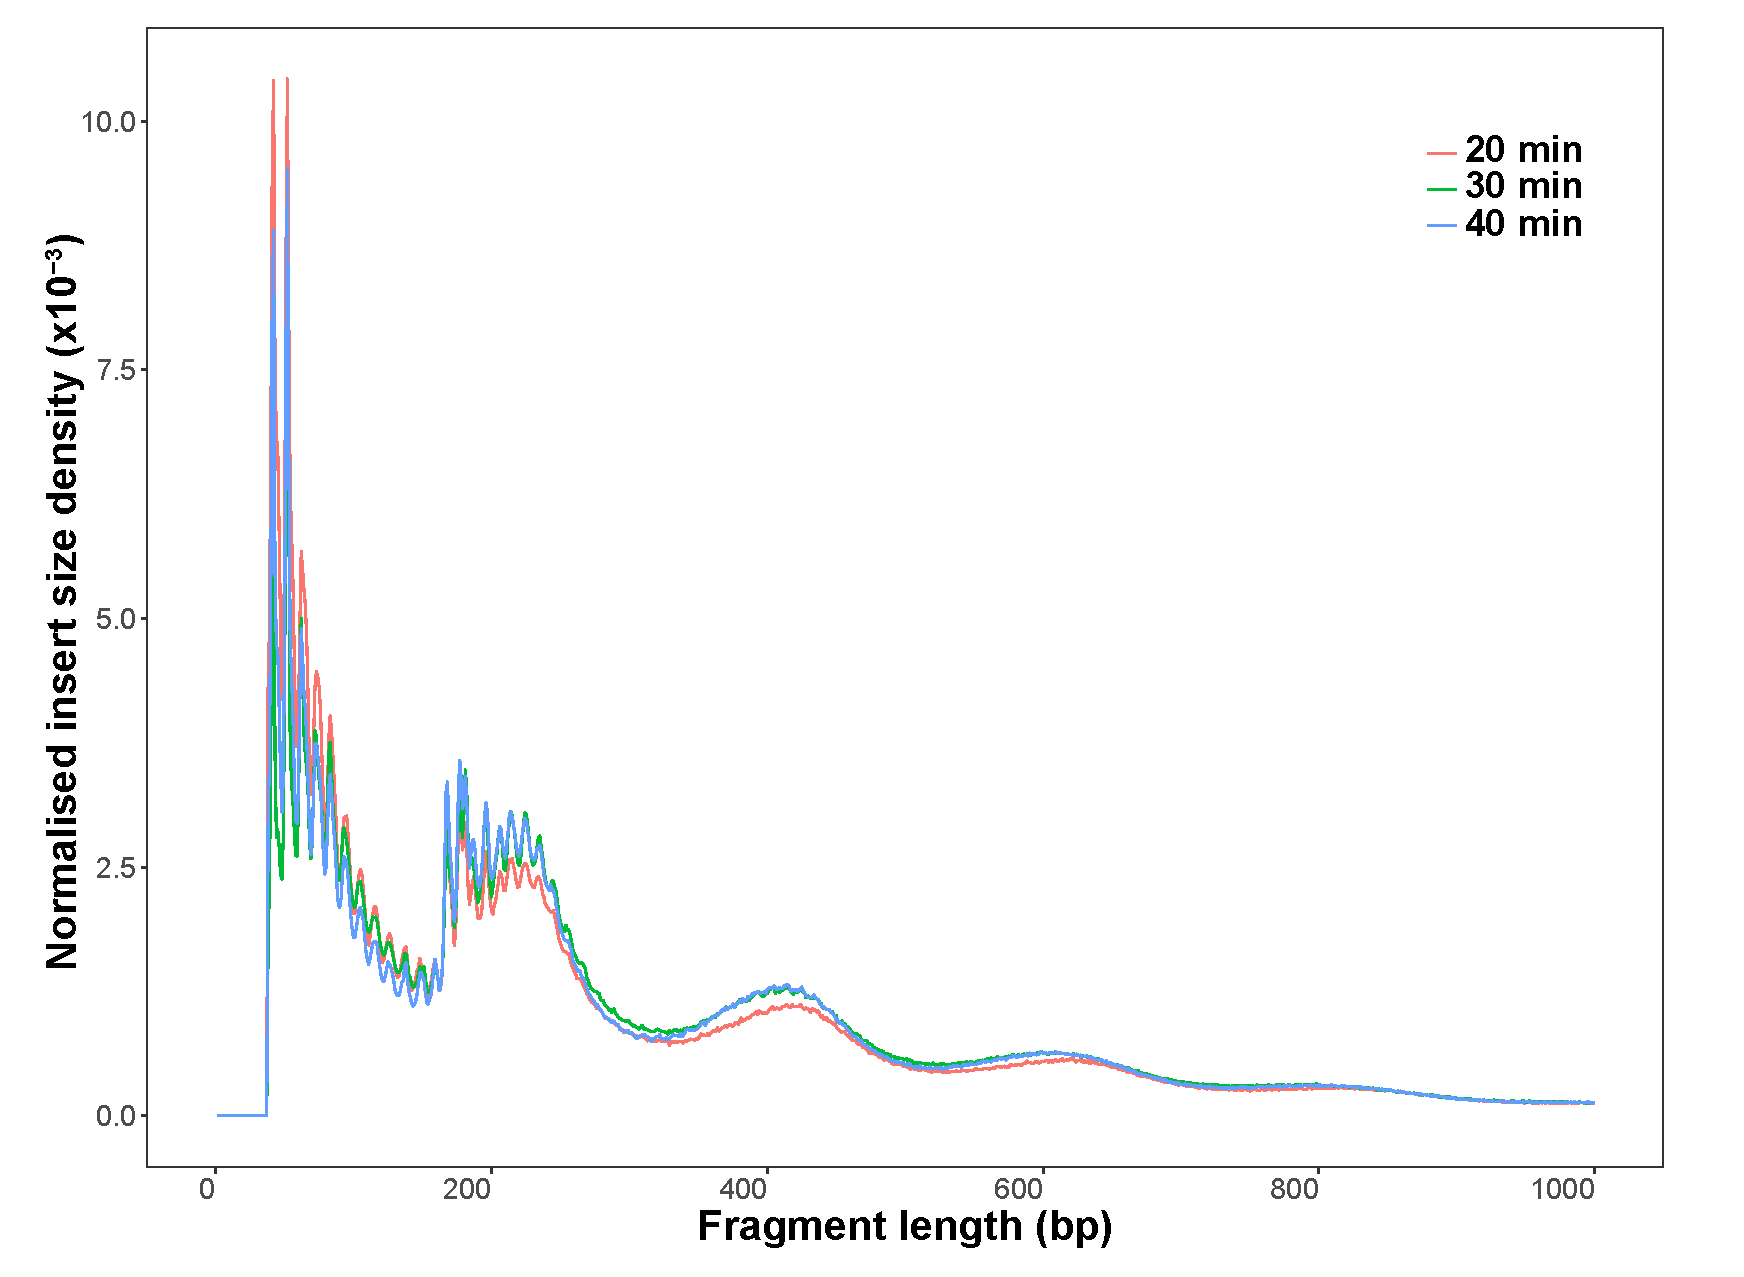
\includegraphics[width=\textwidth]{./Results1/pdfs/ATAC_CD8_fragment_size_distribution_20_30_40min}
\caption{\textbf{}}
% The percentage sign indicated that the other subfig goes side by side
\end{subfigure}%
\begin{subfigure}{0.5\textwidth}
\centering
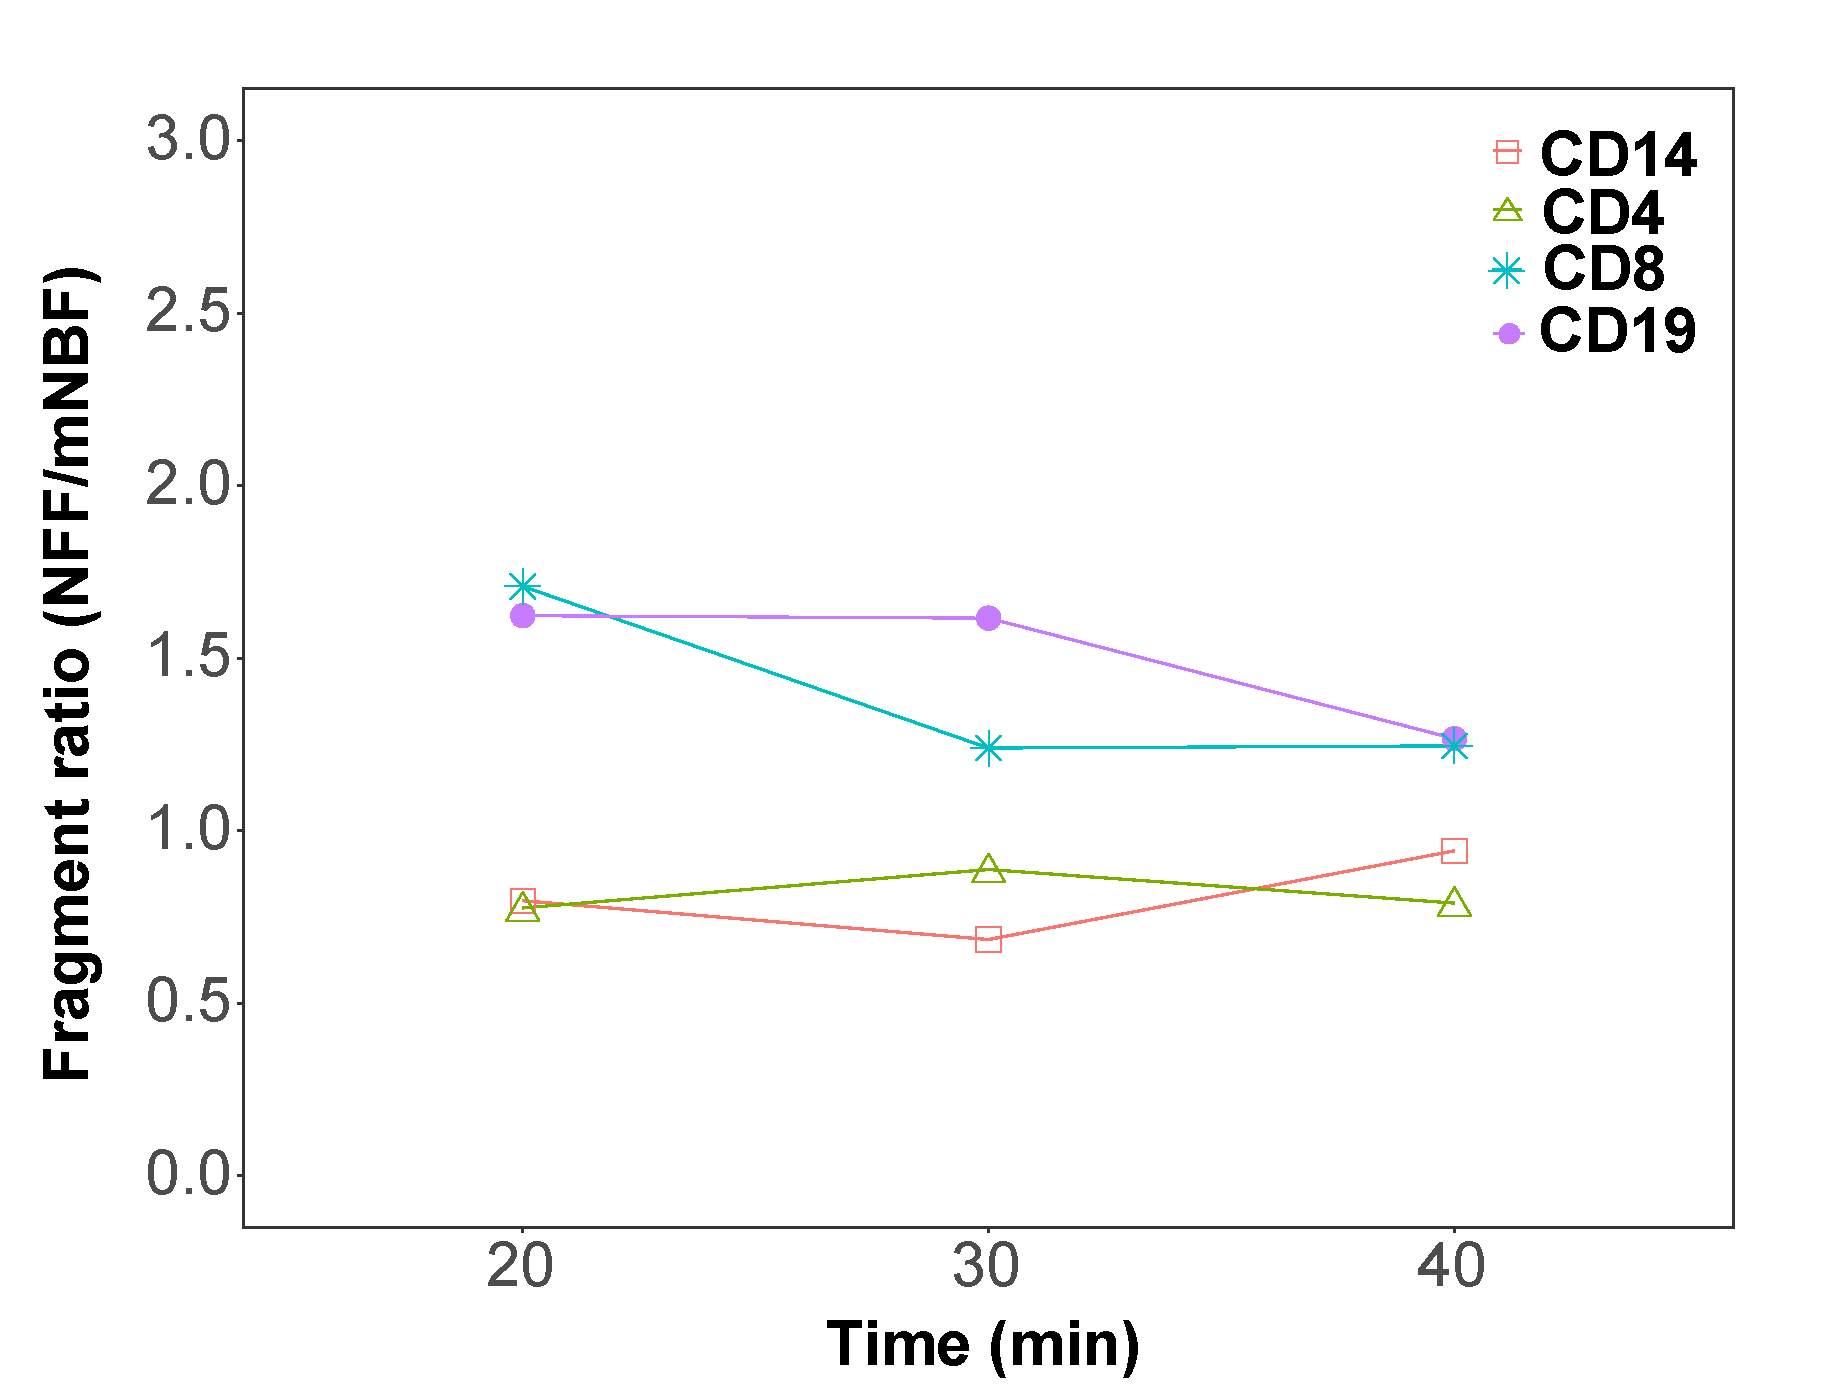
\includegraphics[width=\textwidth]{./Results1/pdfs/ATAC_ratio_short_long_fragments_mononucleosomes_20_30_40_min}
\caption{\textbf{}}
\end{subfigure} \\
\begin{subfigure}{0.5\textwidth}
\centering
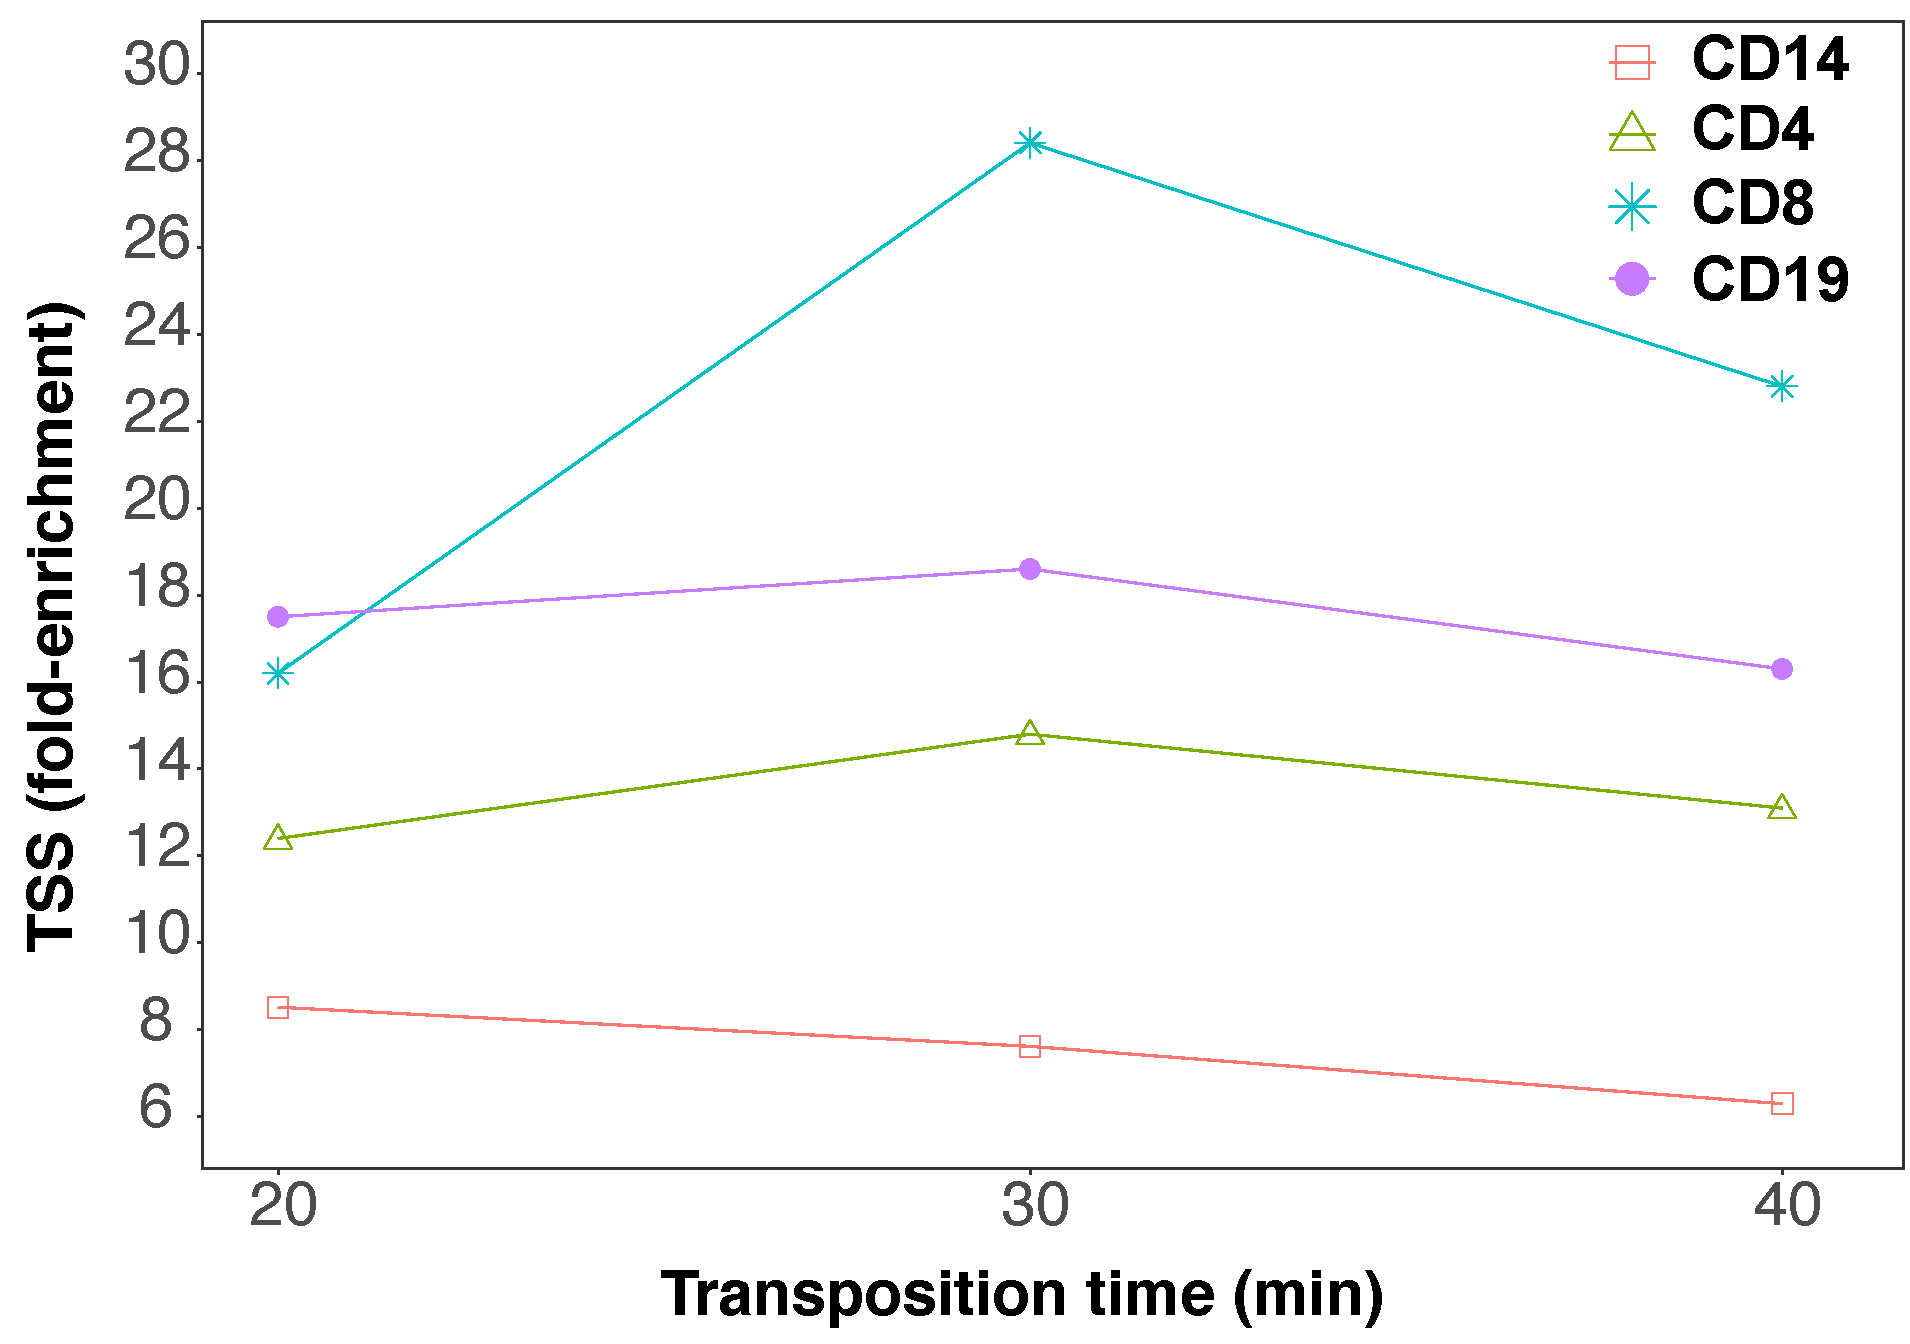
\includegraphics[width=\textwidth]{./Results1/pdfs/ATAC_TSS_vs_transposition_times}
\caption{\textbf{}} % to add text to the figure name
\end{subfigure}%
\begin{subfigure}{0.5\textwidth}
	\centering
	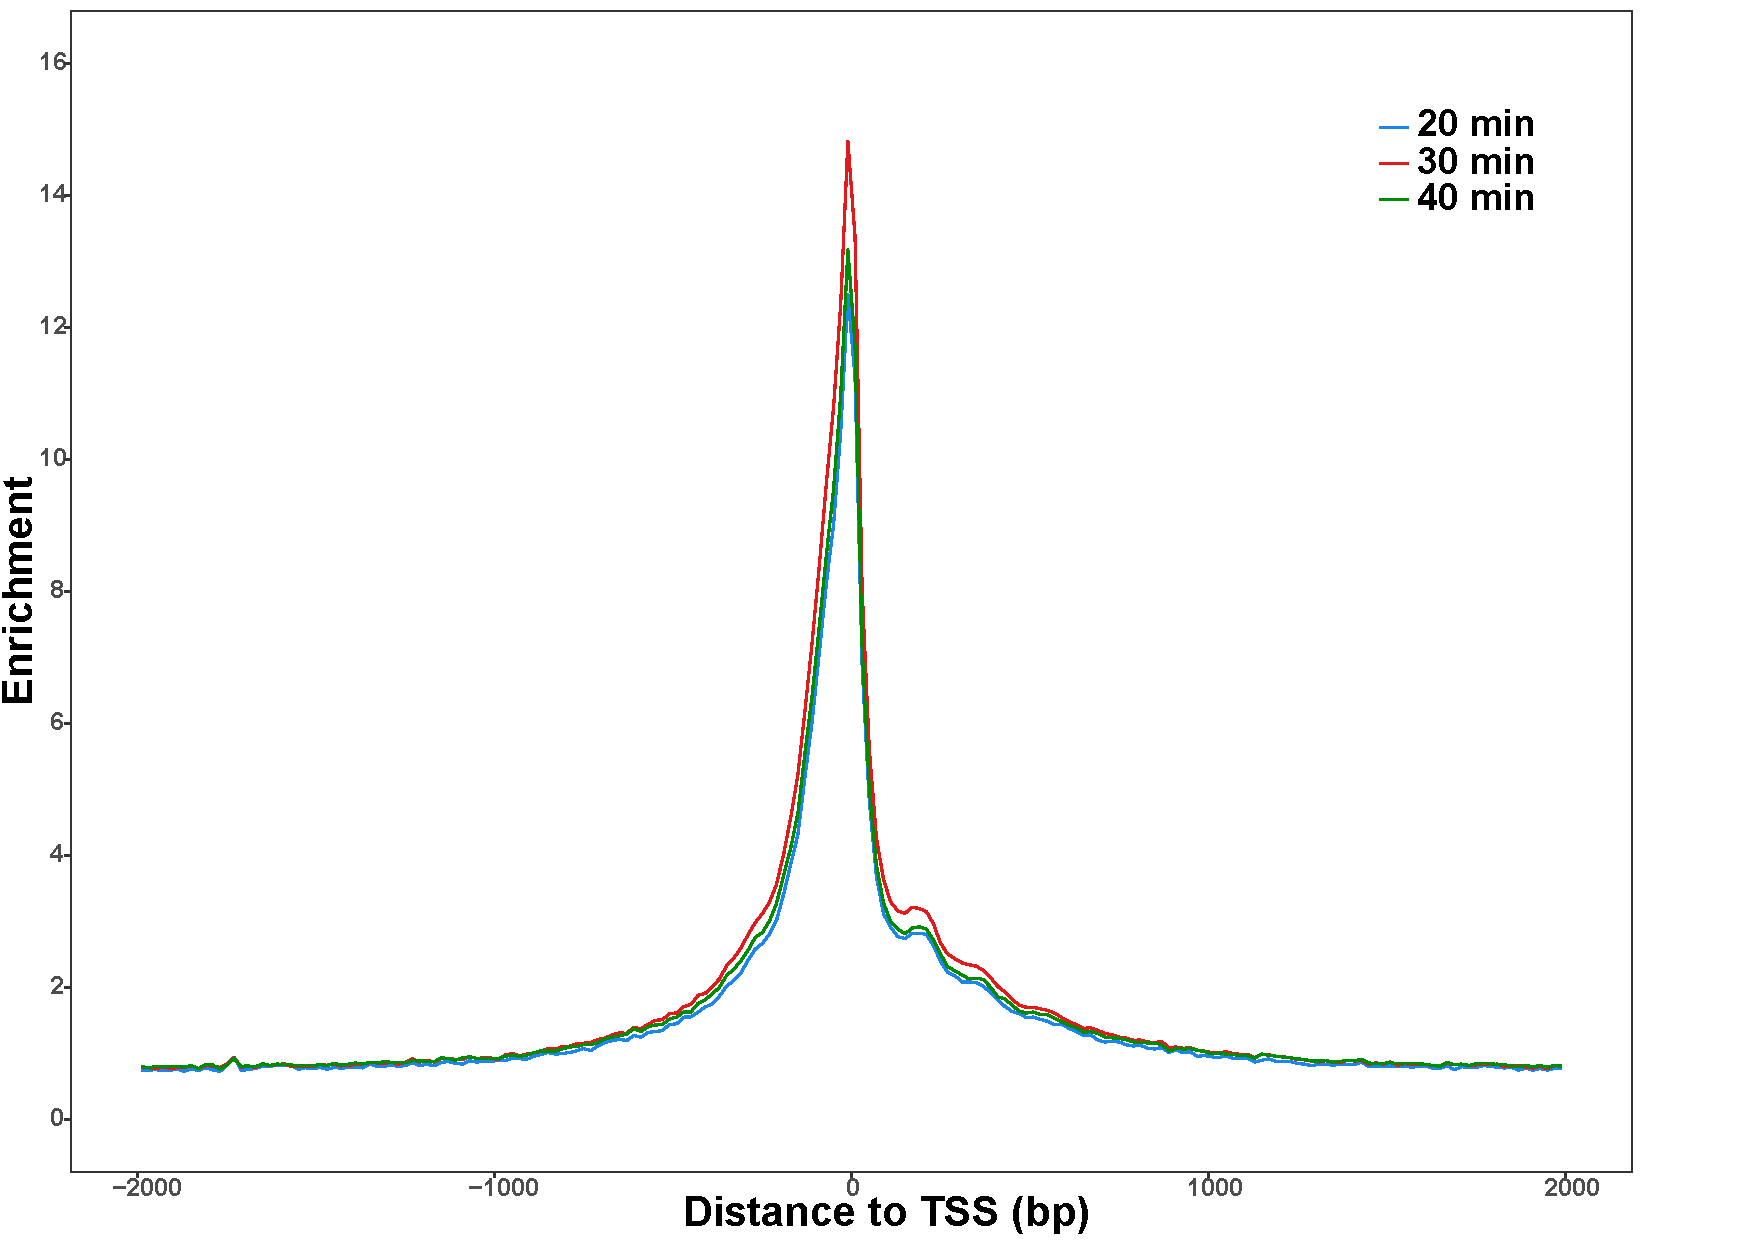
\includegraphics[width=\textwidth]{./Results1/pdfs/ATAC_optimisation_CD4_20_30_40_min_tss_enrichment}
	\caption{\textbf{}} % to add text to the figure name
\end{subfigure}
\caption[Assessment of the effect of transposition times on the ATAC-seq measurements]{\textbf{Assessment of the effect of transposition times on the ATAC-seq measurements}. (A) Representative plot of the ATAC-seq fragment sizes density distribution following 20, 30 and 40 min of transposition in CD8$^+$ cells. Changes across different transposition times in CD14$^+$ monocytes, CD4$^+$, CD8$^+$ and CD19$^+$ cells of (B) the ratio between ATAC-seq nucleosome-free fragments (NFF) (fragments $\leq$150bp) and mono-nucleosome bound fragments (mNBF) ($>$151bp) and (C) TSS fold-enrichment. (D) CD4$^+$ cells enrichment of ATAC-seq fragments for different transposition times across the TSS of all Ensembl genes.}
\label{figure:Transposition_times_ATAC}
\end{figure} 

This variation in NFF/mNBF did not significantly impact the signal-to-noise ratio, with the largest TSS enrichment values corresponding to 30 min in three cell types (Figure \ref{figure:Transposition_times_ATAC}C and D) and the major differences found across cell types. Differences between TSS fold-enrichments at 30 and 40 min were very modest and did not differ in more than 4 units in CD8 $^+$ cells, where the largest variation was found. Before performing this formal comparison of transposition times, some sample recruitment had already been conducted using ATAC-seq with transposition for 40 min, as it was found to be the most appropriate condition based on the relative abundance of DNA fragment sizes profiles from the pre-sequencing library quality control. Although this analysis suggested 30 min as the best condition for the majority of the cell types tested in this single repetition, the differences between 30 min and 40 min were minor and therefore for consistency across the cohort 40 min was used for all other patient samples using ATAC-seq. 




\subsection{Comparison of ATAC-seq with Fast-ATAC protocol}
\label{Fast_ATAC}

An improved Fast-ATAC protocol from Corces and colleagues \parencite{Corces2016} was reported whilst the work in this thesis was being undertaken and was compared with the ATAC-seq protocol from Buenrostro and colleagues \parencite{Buenrostro2013}. The aim was to confirm the two main reported advantages of Fast-ATAC, namely reduction of mitochondrial reads and signal enhancement, before implementing it as the replacement for the current ATAC-seq protocol in use to process patient and control samples (Chapter \ref{ch:Results2} cohort 1A in Tables \ref{tab:Summary_all_cohorts}, \ref{tab:Psoriasis_cohort_metadata} and \ref{tab:Control_cohort_metadata}). Fast-ATAC was conducted in one healthy volunteer sample included in cohort 1B from Chapter \ref{ch:Results2} (Tables \ref{tab:Summary_all_cohorts} and \ref{tab:Control_cohort_metadata}). Fast-ATAC was specifically optimised for haematopoietic cells and used 30 min of transposition. Thus, for consistency, Fast-ATAC samples were here compared to the ATAC-seq library from Section \ref{ATACseq} transposed for 30 min in the same four cell types.


\begin{figure}[htbp]
\centering
\begin{subfigure}{0.5\textwidth}
\centering
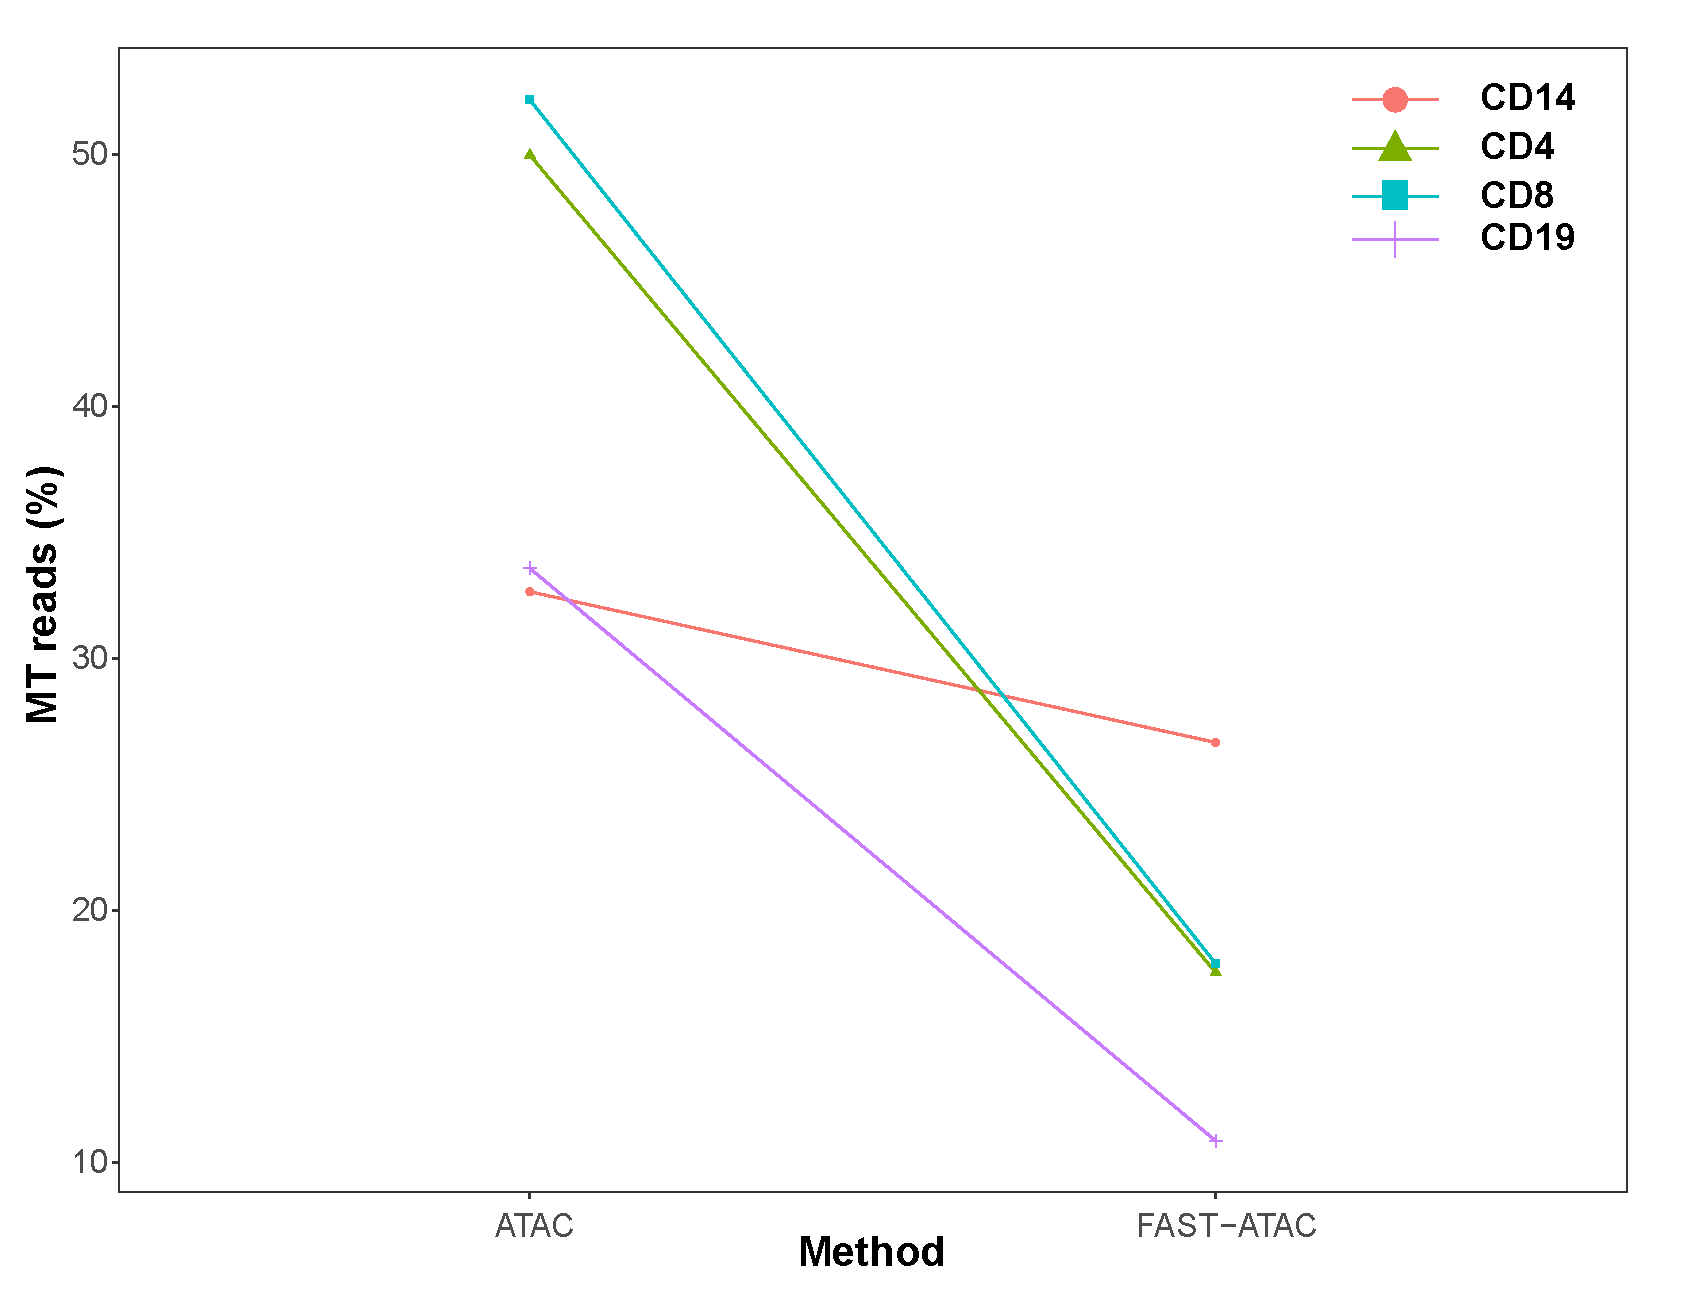
\includegraphics[width=\textwidth]{./Results1/pdfs/ATAC_vs_FAST_ATAC_percnt_MT_reads_dotplot}
\caption{\textbf{}}
% The percentage sign indicated that the other subfig goes side by side
\end{subfigure}%
\begin{subfigure}{0.5\textwidth}
\centering
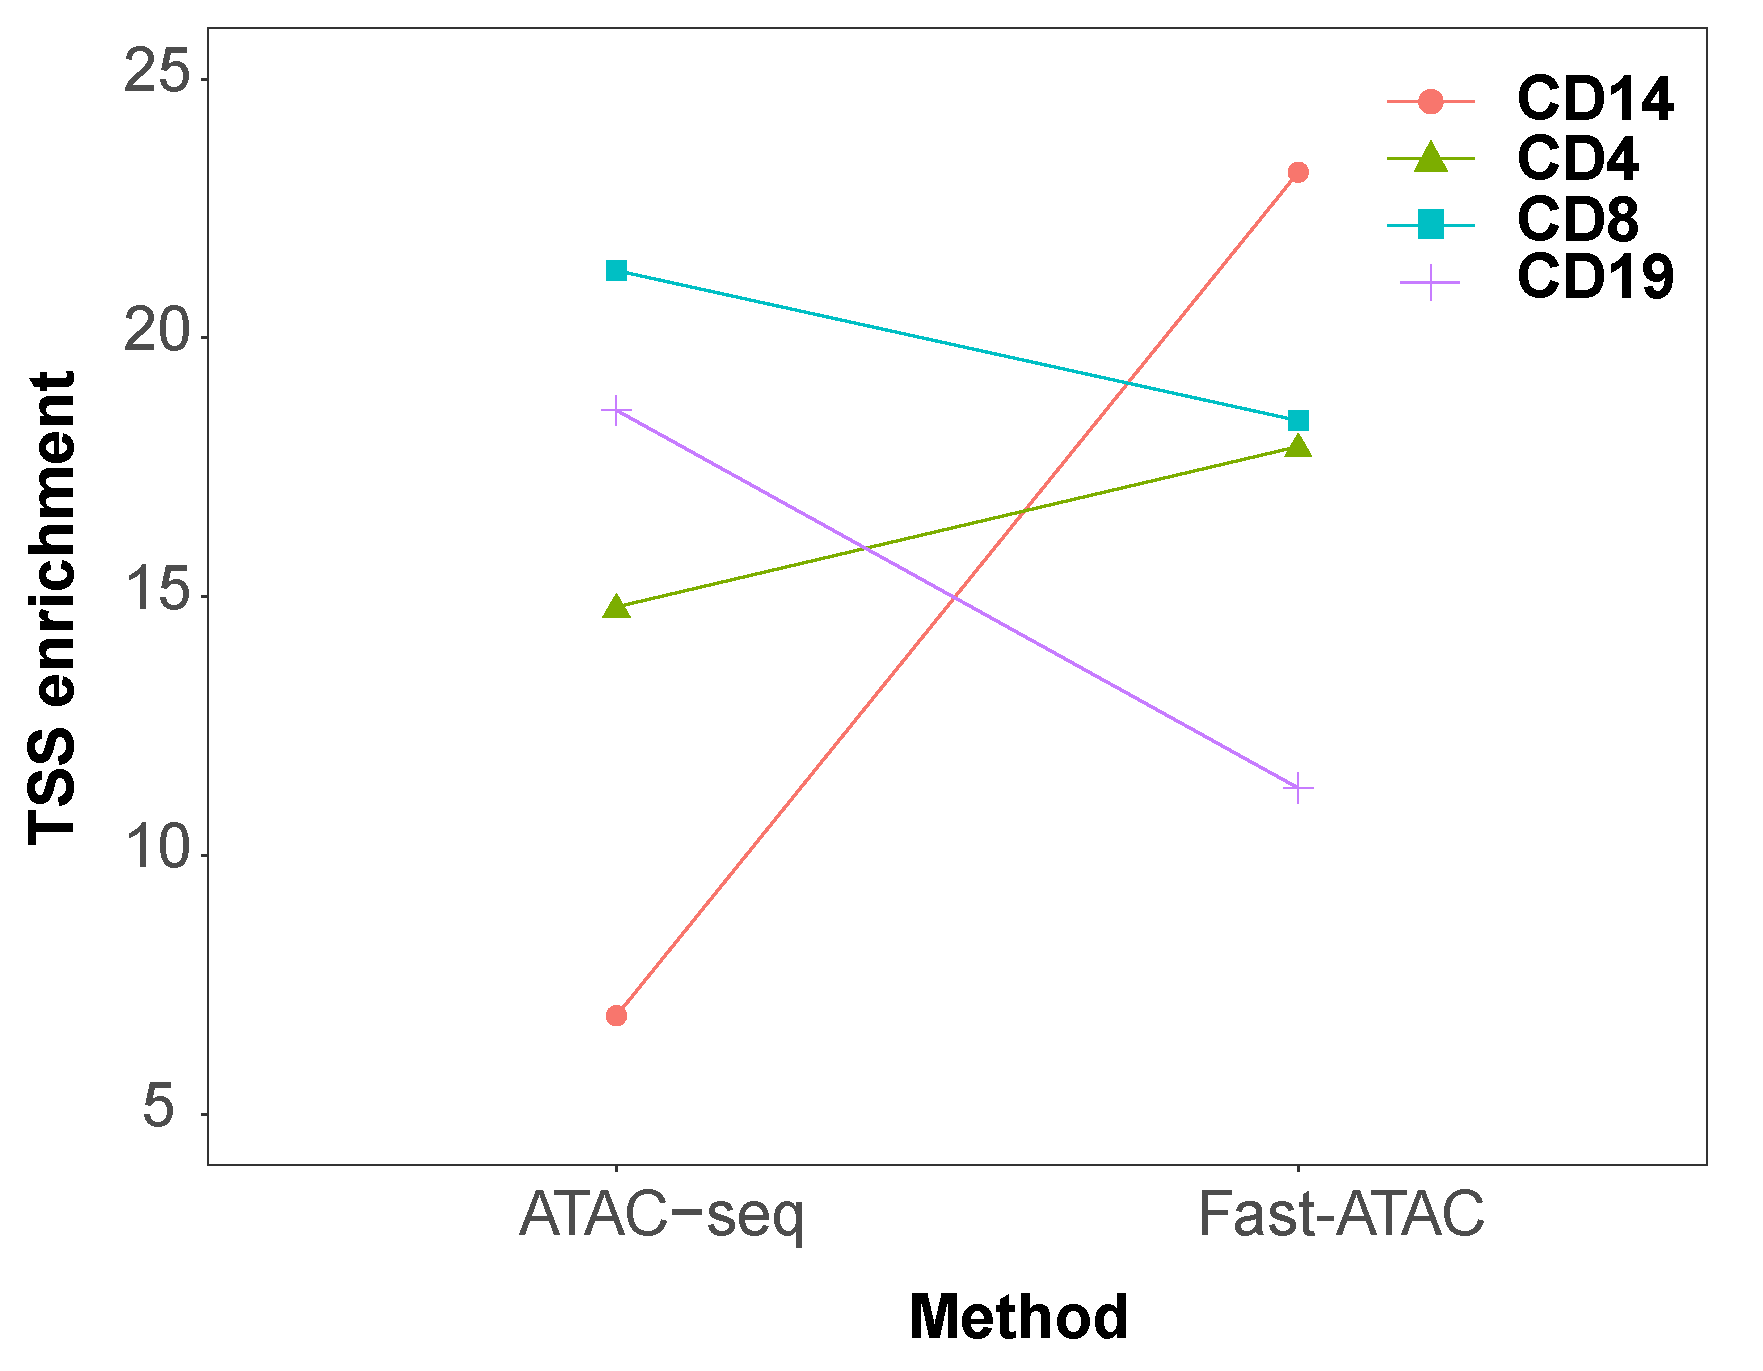
\includegraphics[width=\textwidth]{./Results1/pdfs/ATAC_vs_FAST_ATAC_tss_dotplot}
\caption{\textbf{}}
\end{subfigure}
\caption[Differences in mitochondrial DNA abundance and TSS enrichment between ATAC-seq and Fast-ATAC protocols.]{\textbf{Differences in mitochondrial DNA abundance and TSS enrichment between ATAC-seq and Fast-ATAC protocols.} Representation of changes in (A) percentage of mitochondrial reads and (B) TSS fold-enrichment between ATAC-seq and Fast-ATAC libraries for CD14$^+$ monocytes, CD4$^+$, CD8$^+$ and CD19$^+$ cells. Fast-ATAC protocol was specifically optimised by Corces and colleagues for hematopoietic cells and recommends 30 min of transposition (\ref{ch:Mat} and Corces \textit{et al.} 2016). Therefore, for consistency, Fast-ATAC samples were compared to the ATAC-seq libraries from Section \ref{ATACseq} transposed for 30 min.}
\label{figure:ATAC_vs_FAST_ATAC}
\end{figure} 

%\ToDo{Prospective analysis comparing all the ATAC-seq vs the Fast-ATAC libraries generated by the end of this thesis (samples presented in Chapters \ref{ch:Results2} and \ref{ch:Results3}) only showed a significant increase in TSS fold-enrichment for the Fast-ATAC protocol in CD4${^+}$ T cells (unpaired Wilcoxon signed-ranked test p-value=0.024) (Figure  \ref{figure:Comparison_ATACseq_vs_fastATAC_all_thesis_samples}A). Conversely, Fast-ATAC significantly reduced the percentage of mitochondrial reads in the four studied cell types (unpaired Wilcoxon signed-ranked test p-values$<$4.1x10$^{-05}$) (Figure  \ref{figure:Comparison_ATACseq_vs_fastATAC_all_thesis_samples}B).}


The percentage of mitochondrial reads in the Fast-ATAC libraries was lower for all cell types analysed compared to ATAC-seq (Figure \ref{figure:ATAC_vs_FAST_ATAC}A). CD4$^+$ and CD8$^+$ cells showed the largest reduction from 50\% to less than 20\% when using ATAC-seq and Fast-ATAC, respectively. With regard to the background signal, differing trends were observed across cell types (Figure \ref{figure:ATAC_vs_FAST_ATAC}B). No change in TSS enrichment was observed for CD14$^+$ monocytes or CD4$^+$ T cells whereas CD8$^+$ and CD19$^+$ cells showed a reduction when using Fast-ATAC compared to ATAC-seq. Overall, the large decrease in mitochondrial reads together with the reduced duration of the experimental protocol supported the replacement of ATAC-seq by Fast-ATAC for future patients recruitment (see Chapter \ref{ch:Results2}). 




\subsection{Limitations of ATAC-seq and Fast-ATAC to assess chromatin accessibility in keratinocytes}
A particular aim of this thesis was to characterise the regulatory landscape in psoriatic keratinocytes, one of the most relevant cell types in this pathophysiology. In order to assess the feasibility of using the ATAC-seq protocol from Buenrostro and colleagues \parencite{Buenrostro2013} (referred to as ATAC 1 in this subsection), epidermis from a psoriatic lesional skin biopsy was isolated, digested with trypsin and filtered through a cell strainer to ensure a single-cell suspension, as detailed in Chapter \ref{ch:Mat}. Cell suspensions obtained from skin biopsies using trypsinisation of the epidermal layer are enriched in keratinocytes, constituting approximately 90\% of the cells \parencite{Haftek1986}.  Approximately 50,000 cells from the suspension were counted and ATAC 1 was performed for two different transposition times (30 and 40 min). %Given the challenge of handling skin biopsies and isolating the epidermis from psoriatic lesional skin, testing the performance of ATAC1 in the clinical sample of interest was considered the best approach.

 Pre-sequencing library quality control to assess the relative abundance of different DNA fragment sizes recapitulated the characteristic ATAC nucleosome pattern every $\sim$200bp resulting from transposition of nucleosome-free and nucleosome-bound DNA in both samples (Figures \ref{figure:PS02_skin_ATAC_QC_assessment}A and \ref{figure:PS2_40min_tapestation}). Following sequencing, calculation of TSS fold enrichment values for the two ibraries demonstrated to be below the acceptable cut-off threshold of 6, with slightly better signal (3.5 fold-enrichment) for the 30 min transposition time (Figure \ref{figure:PS02_skin_ATAC_QC_assessment}B). Fragment size distribution using NGS data from the same libraries was consistent with the pre-sequencing assessment, showing approximately equal abundance of the NFF and mono-nucleosome fragments for both transposition times (Figure \ref{figure:PS02_skin_ATAC_QC_assessment}C). Similar abundance of NFF and NBF can also be found in good quality libraries with TSS fold-enrichment above 6 (as seen previously). However, in this case, the extremely low TSS enrichments could suggest that a significant proportion of the NFF in these libraries are free-DNA released by apoptotic cells as a result of the trypsinisation step. Moreover, poor lysis of the keratinocytes may also result in inefficient access of the transposase into the nuclei compartment. This would cause under-transposition and greater NBF abundance when compared to NFF, which in this case may not be revealed as a result of large amounts of NFF being generated from tagmented free-DNA.



\begin{figure}[htbp]
\centering
\begin{subfigure}{0.7\textwidth}
\centering
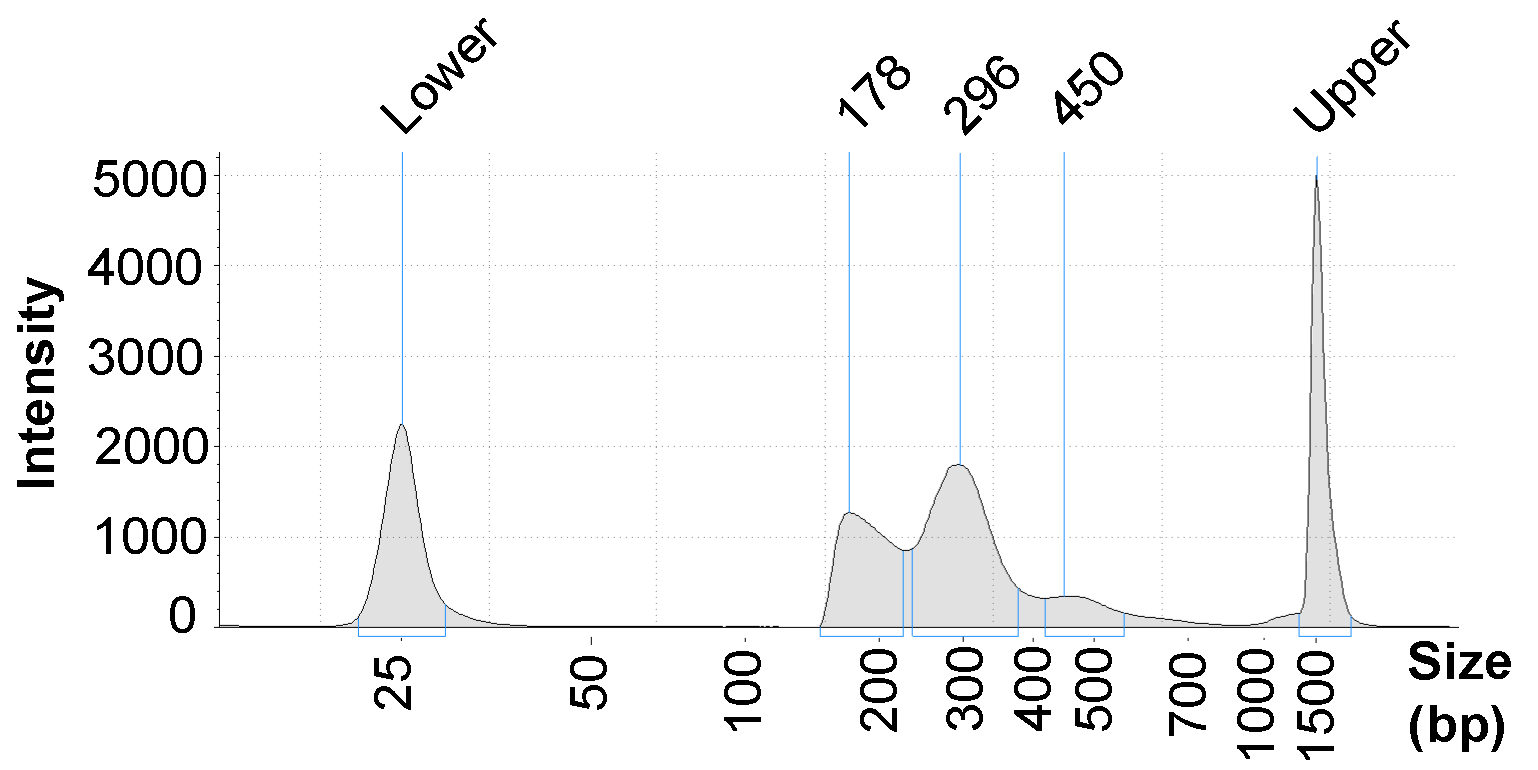
\includegraphics[width=\textwidth]{./Results1/pdfs/ATAC_PS02_tapestation_30min}
\caption{\textbf{}}
\end{subfigure}
\begin{subfigure}{0.45\textwidth}
\centering
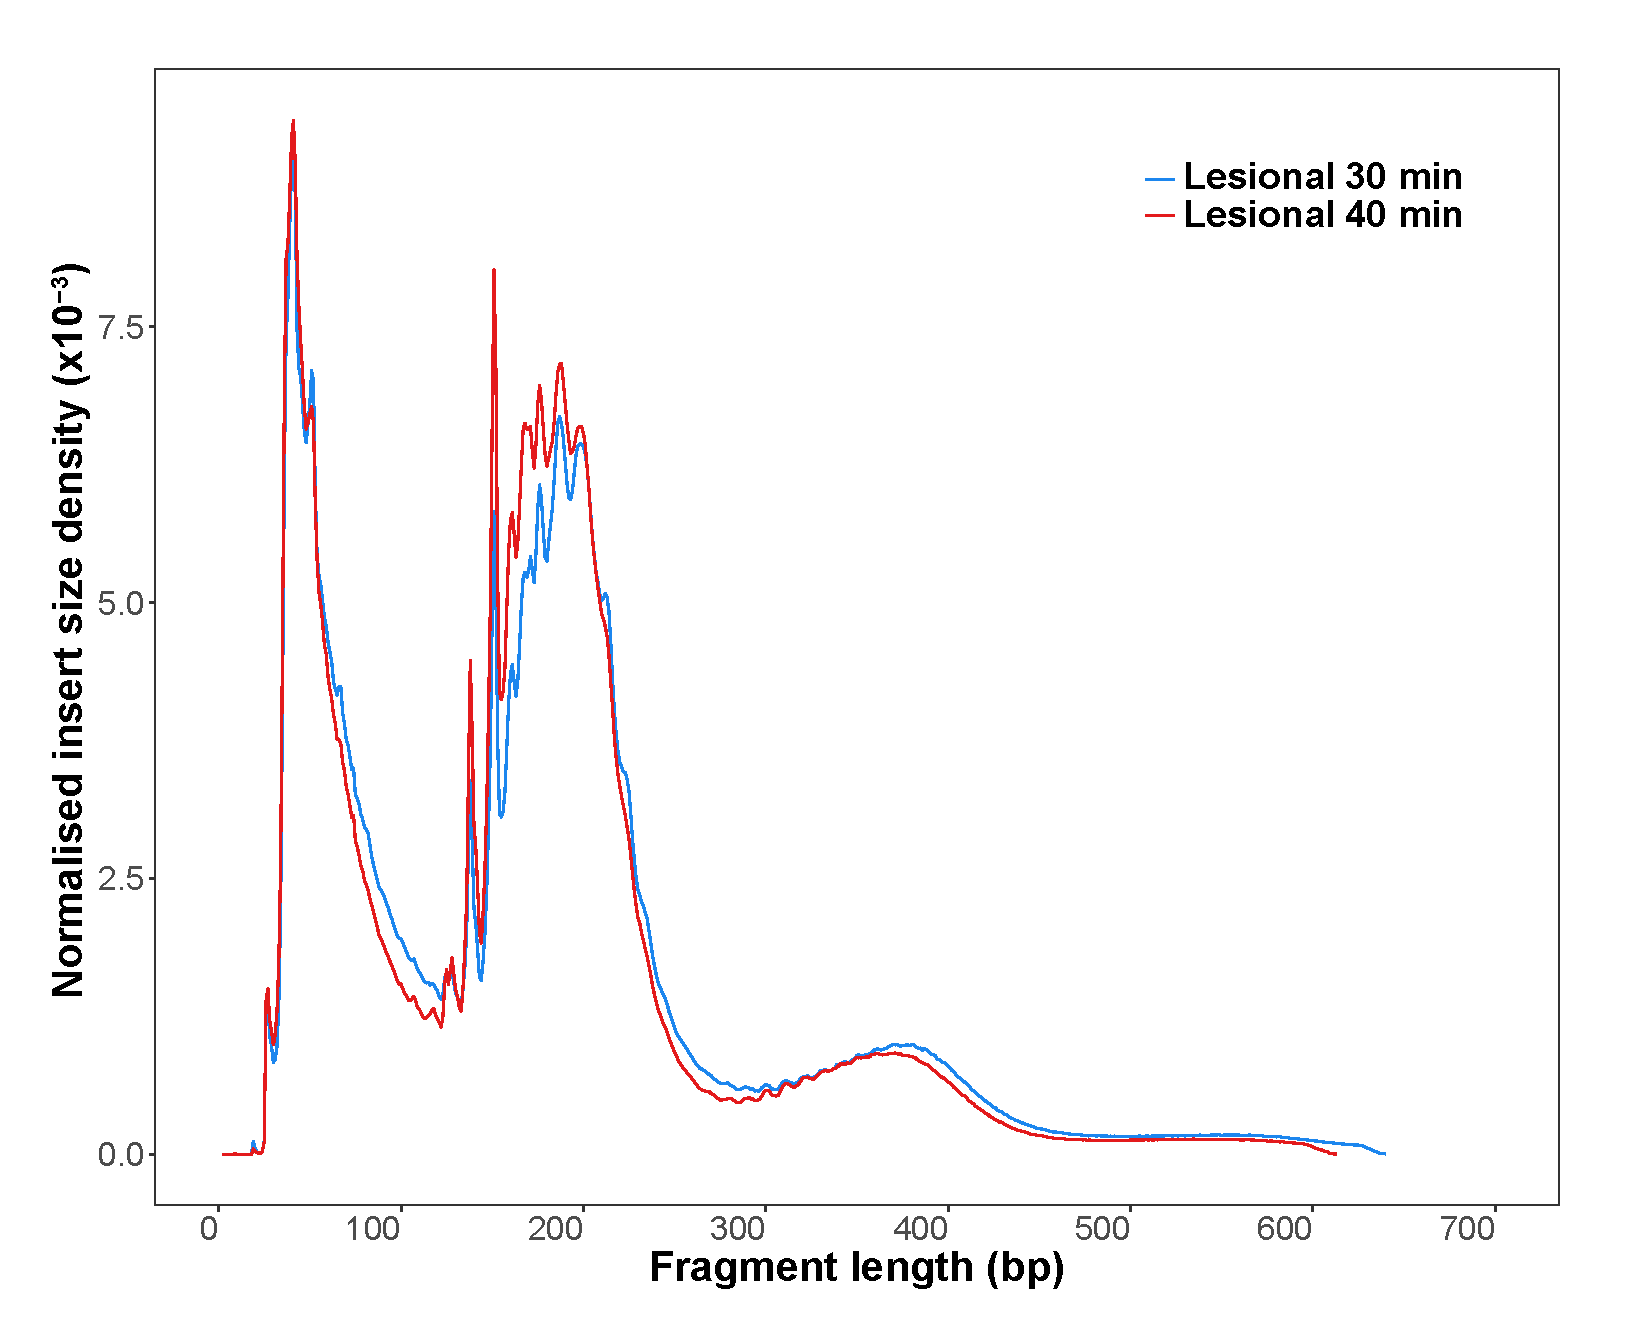
\includegraphics[width=\textwidth]{./Results1/pdfs/ATAC_PS-2_30_40_min_fragment_size_distribution}
\caption{\textbf{}}
\end{subfigure}%
\begin{subfigure}{0.45\textwidth}
\centering
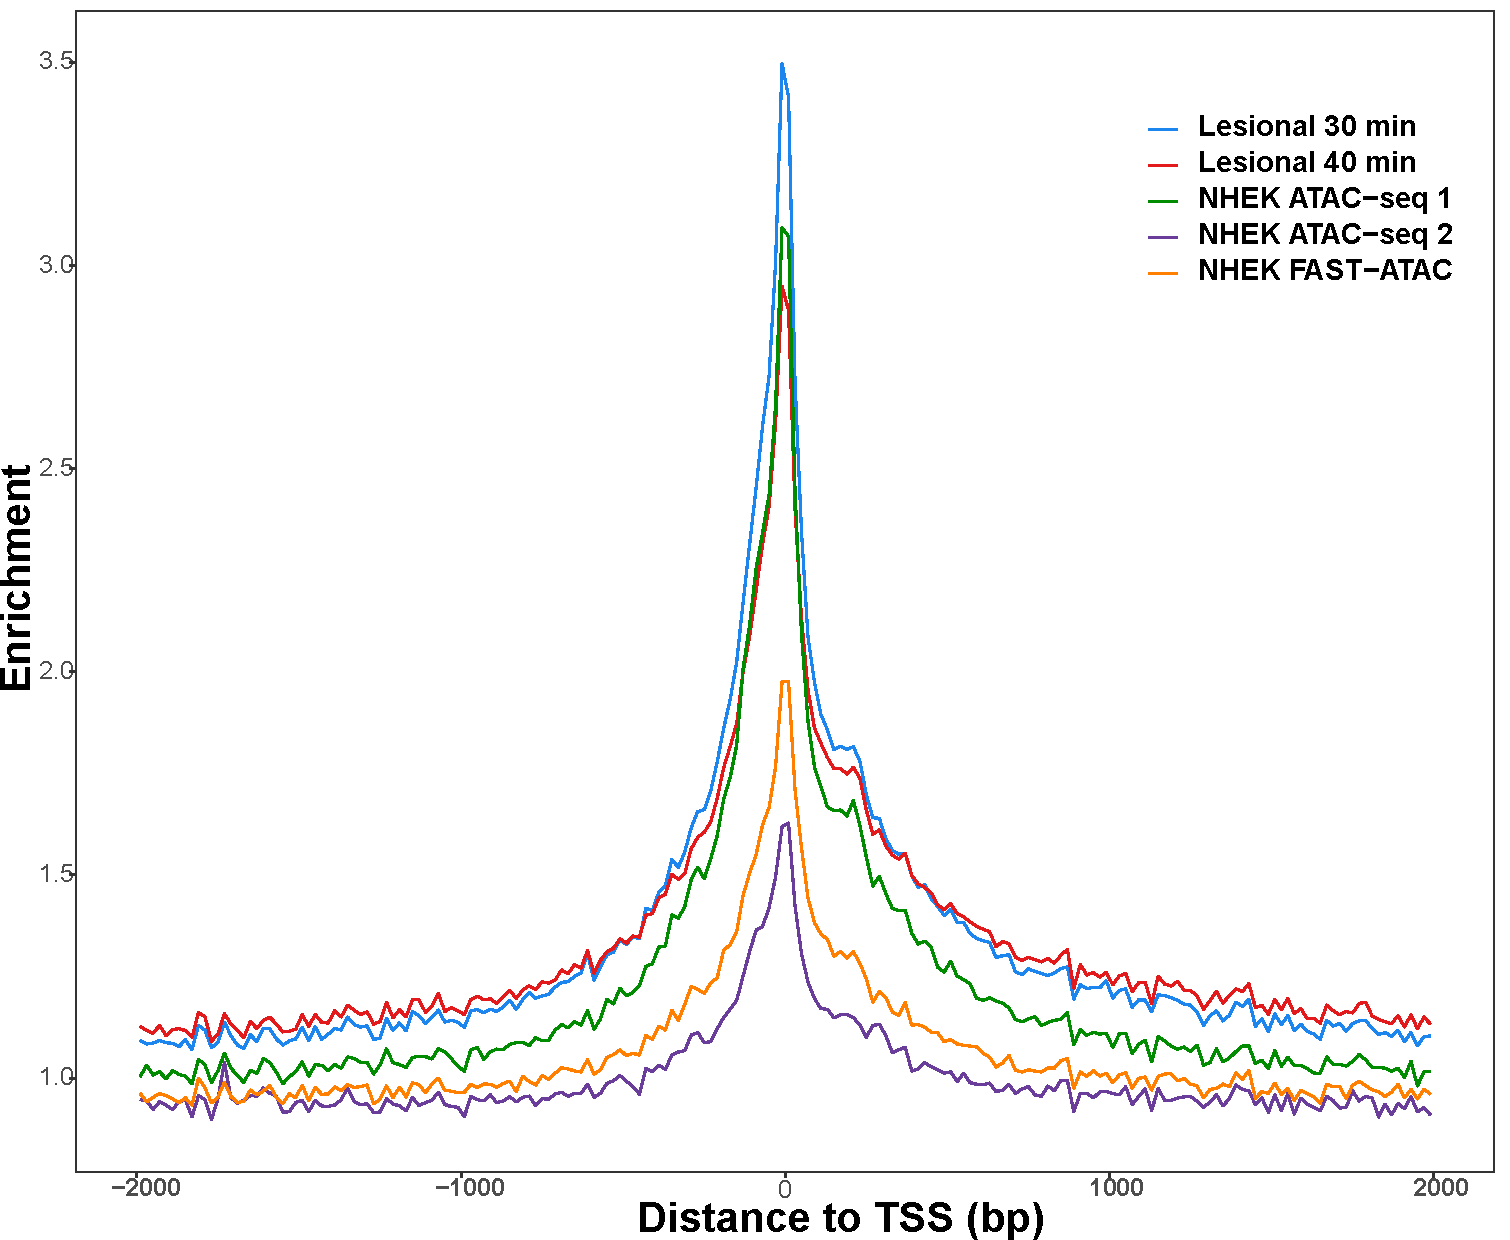
\includegraphics[width=\textwidth]{./Results1/pdfs/ATAC_skin_TSS_enrichment_PS02_30_40min_NHEK_ATAC1_ATAC_2_FAST_ATAC}
\caption{\textbf{}} % to add text to the figure name
\end{subfigure}
\caption[Quality control assessment of different ATAC protocols in keratinocytes from a psoriatic lesion and NHEKs.]{\textbf{Quality control assessment of different ATAC protocols in keratinocytes from a psoriatic lesion and NHEKs.} (A) Pre-sequencing quality control showing relative abundance of different DNA fragment sizes in the ATAC libraries generated in 50,000 cells from a suspension of keratinocytes isolated from lesional skin of one psoriasis patient. Cells from the same suspension were used to test two transposition times (30 and 40 min) and the profile for the 30 min library is shown here. The corresponding pre-sequencing profile for the sample transposed for 40 min is included in Figure \ref{figure:PS2_40min_tapestation}. (B) Fold-enrichment of ATAC fragments across the Ensembl annotated TSS from the ATAC 1 psoriasis lesional keratinocytes libraries, previously mentioned in (A), and NHEK libraries generated by performing ATAC 1, ATAC 2 and Fast-ATAC protocols directly on adherent cells cultured in 96-well plates. (C) Density distribution of sequenced fragments for ATAC 1 libraries in (A) and Figure \ref{figure:PS2_40min_tapestation}.}
\label{figure:PS02_skin_ATAC_QC_assessment}
\end{figure} 


Following the ATAC-seq protocol, a modified ATAC-seq version for keratinocytes by Bao and colleagues (named ATAC 2 in this subsection) and the Fast-ATAC protocols were published \parencite{Bao2015, Corces2016}. Interestingly, Bao's protocol was performed directly on NHEKs adhered to the cell culture plate, avoiding the trypsinisation step that could compromise cell viability. This protocol reduced the percentage of NP-40 (weaker lysis) but increased the amount of Tn5 enzyme per cell, which may address potential under-transposition due to insufficient Tn5 availability. In line with Bao and colleagues approach, the three ATAC protocols (ATAC 1 30 min, ATAC 2 and Fast-ATAC using C1 conditions, Table \ref{tab:ATAC_skin_optimisation_protocols}) were tested directly on keratinocytes isolated from skin biopsies and/or NHEKs cultured on 96-well plates to avoid the trypsinisation step and the sunsequent impact of dead cells in data quality. For this purpose, the cell suspension of epidermal keratinocytes obtained skin biopsies were cultured for 3h in a 96-well plate following a washing step to remove remaining non-viable cells. This procedure is known as adherence assay and allows the isolation of viable undifferentiated keratinocytes. Similarly, 50,000 NHEKs were cultured per well and used as control to test the performance of the different protocols in keratinocyte cells. 


\begin{table}[htbp]
%\setlength{\tabcolsep}{20pt}
%\renewcommand{\arraystretch}{1.5}
\begin{tabular}{@{} c c c}
\toprule
\textbf{Protocol}   & \textbf{Lysis and} & \textbf{Key parameters} \\
                    & \textbf{transposition} &  \\
\midrule
\midrule
ATAC 1          & Two steps & 0.1\% NP-40 and 2.5$\micro$L Tn5  \\
\parencite{Buenrostro2013} && \\
&&\\
ATAC 2          &Two steps   & 0.05\% NP-40 and 5$\micro$L Tn5  \\
\parencite{Bao2015} &&\\
&&\\
                                 &             & C1$^\ast$: 0.01\% digitonin, 2.5$\micro$L Tn5 \\
 Fast-ATAC                       &             & C2: 0.01\% digitonin, 0.5$\micro$L Tn5 \\
\parencite{Corces2016}           & One step    & C3: 0.025\% digitonin, 0.5$\micro$L Tn5 \\
													       &             & C4: 0.025\% digitonin, 2.5 $\micro$L Tn5 \\
\bottomrule
\end{tabular}
\medskip %gap
\caption[Description of the most relevant parameter from the ATAC-seq and FAST-ATAC protocols assayed in NHEK and skin biopsies.]{\textbf{Description of the most relevant parameter from the ATAC-seq and FAST-ATAC protocols assayed in NHEK and skin biopsies.}Transposition times for all protocols was 30 min. $^\ast$ corresponds to the original Fast-ATAC conditions from Corces \textit{et al.} 2016.}
\label{tab:ATAC_skin_optimisation_protocols}
\end{table}
\bigskip %bigger space

For the three tested protocols, the NHEKs library size distribution of sequenced fragments showed the presence of NFF and a poorly defined nucleosome pattern, particularly for the ATAC 2 protocol (Figure \ref{figure:Skin_ATAC1__ATAC2_Fast_ATAC_Omni_ATAC_QC_assessment}A). Moreover, the TSS enrichment was under the recommended cut-off of 6 in skin biopsy keratinocytes and NHEKs libraries from the three protocols (Figures \ref{figure:PS02_skin_ATAC_QC_assessment}C and \ref{figure:TSS_skin_biopsies}). Potential poor lysis was further addressed through additional modifications of the Fast-ATAC protocol by increasing the concentration of detergent NP-40 and in combination with the standard or lower Tn5 amounts (2.5 and 0.5 $\micro$L, respectively)(Table \ref{tab:ATAC_skin_optimisation_protocols} C2 to 4). Library quality control prior to sequencing to assess the relative abundance of different DNA fragment sizes failed to show the characteristic nucleosome pattern profile expected in ATAC for any of the three tested conditions, and therefore NGS was not performed (Figure \ref{figure:NHEK_tapestation}A, B and C).

 

\begin{figure}[htbp]
\centering
\begin{subfigure}{0.48\textwidth}
\centering
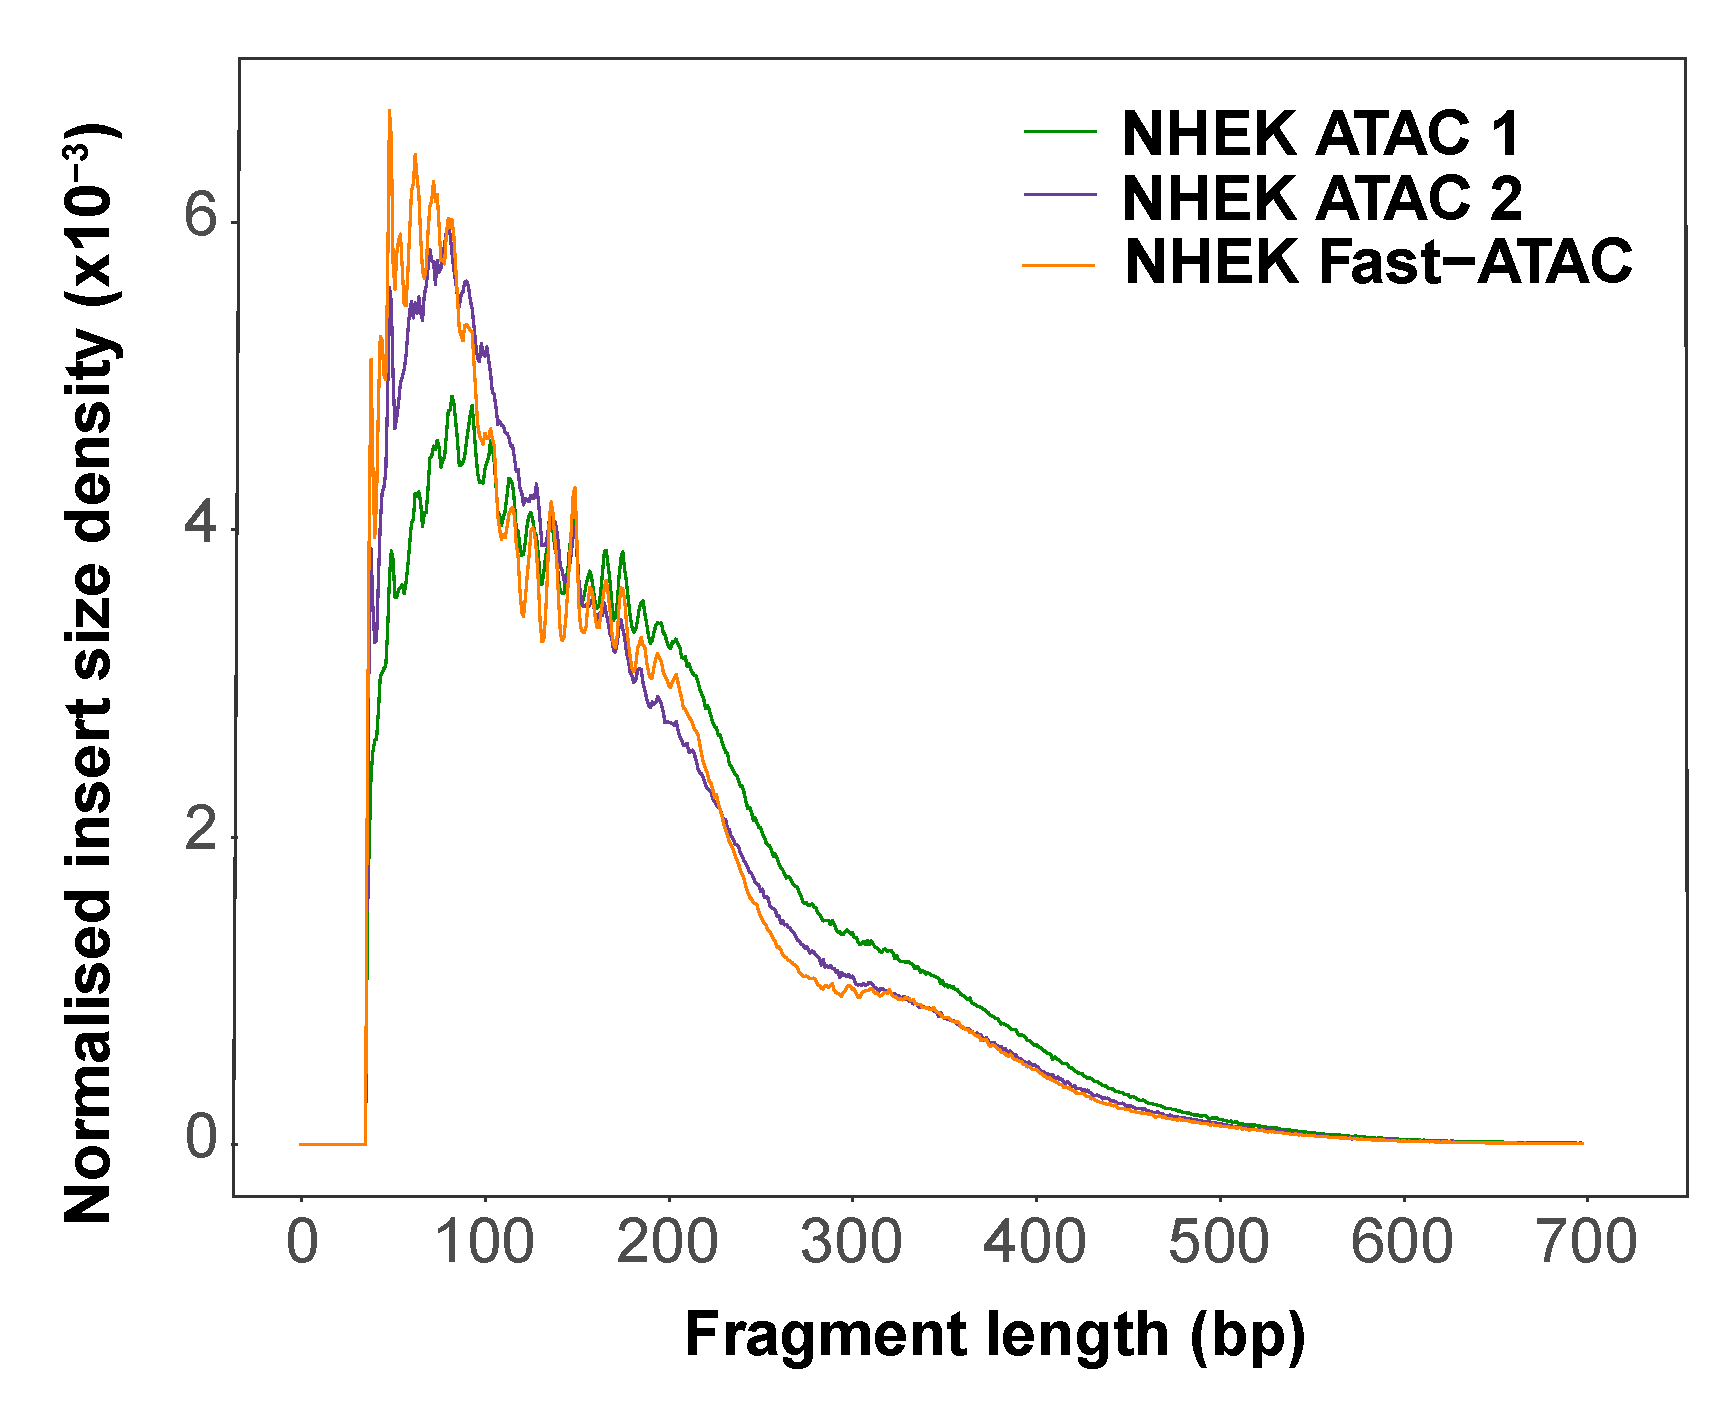
\includegraphics[width=\textwidth]{./Results1/pdfs/ATAC_NHEK_ATAC1_ATAC2_FAST_ATAC_fragment_size_distribution}
\caption{\textbf{}}
\end{subfigure}%
\begin{subfigure}{0.48\textwidth}
\centering
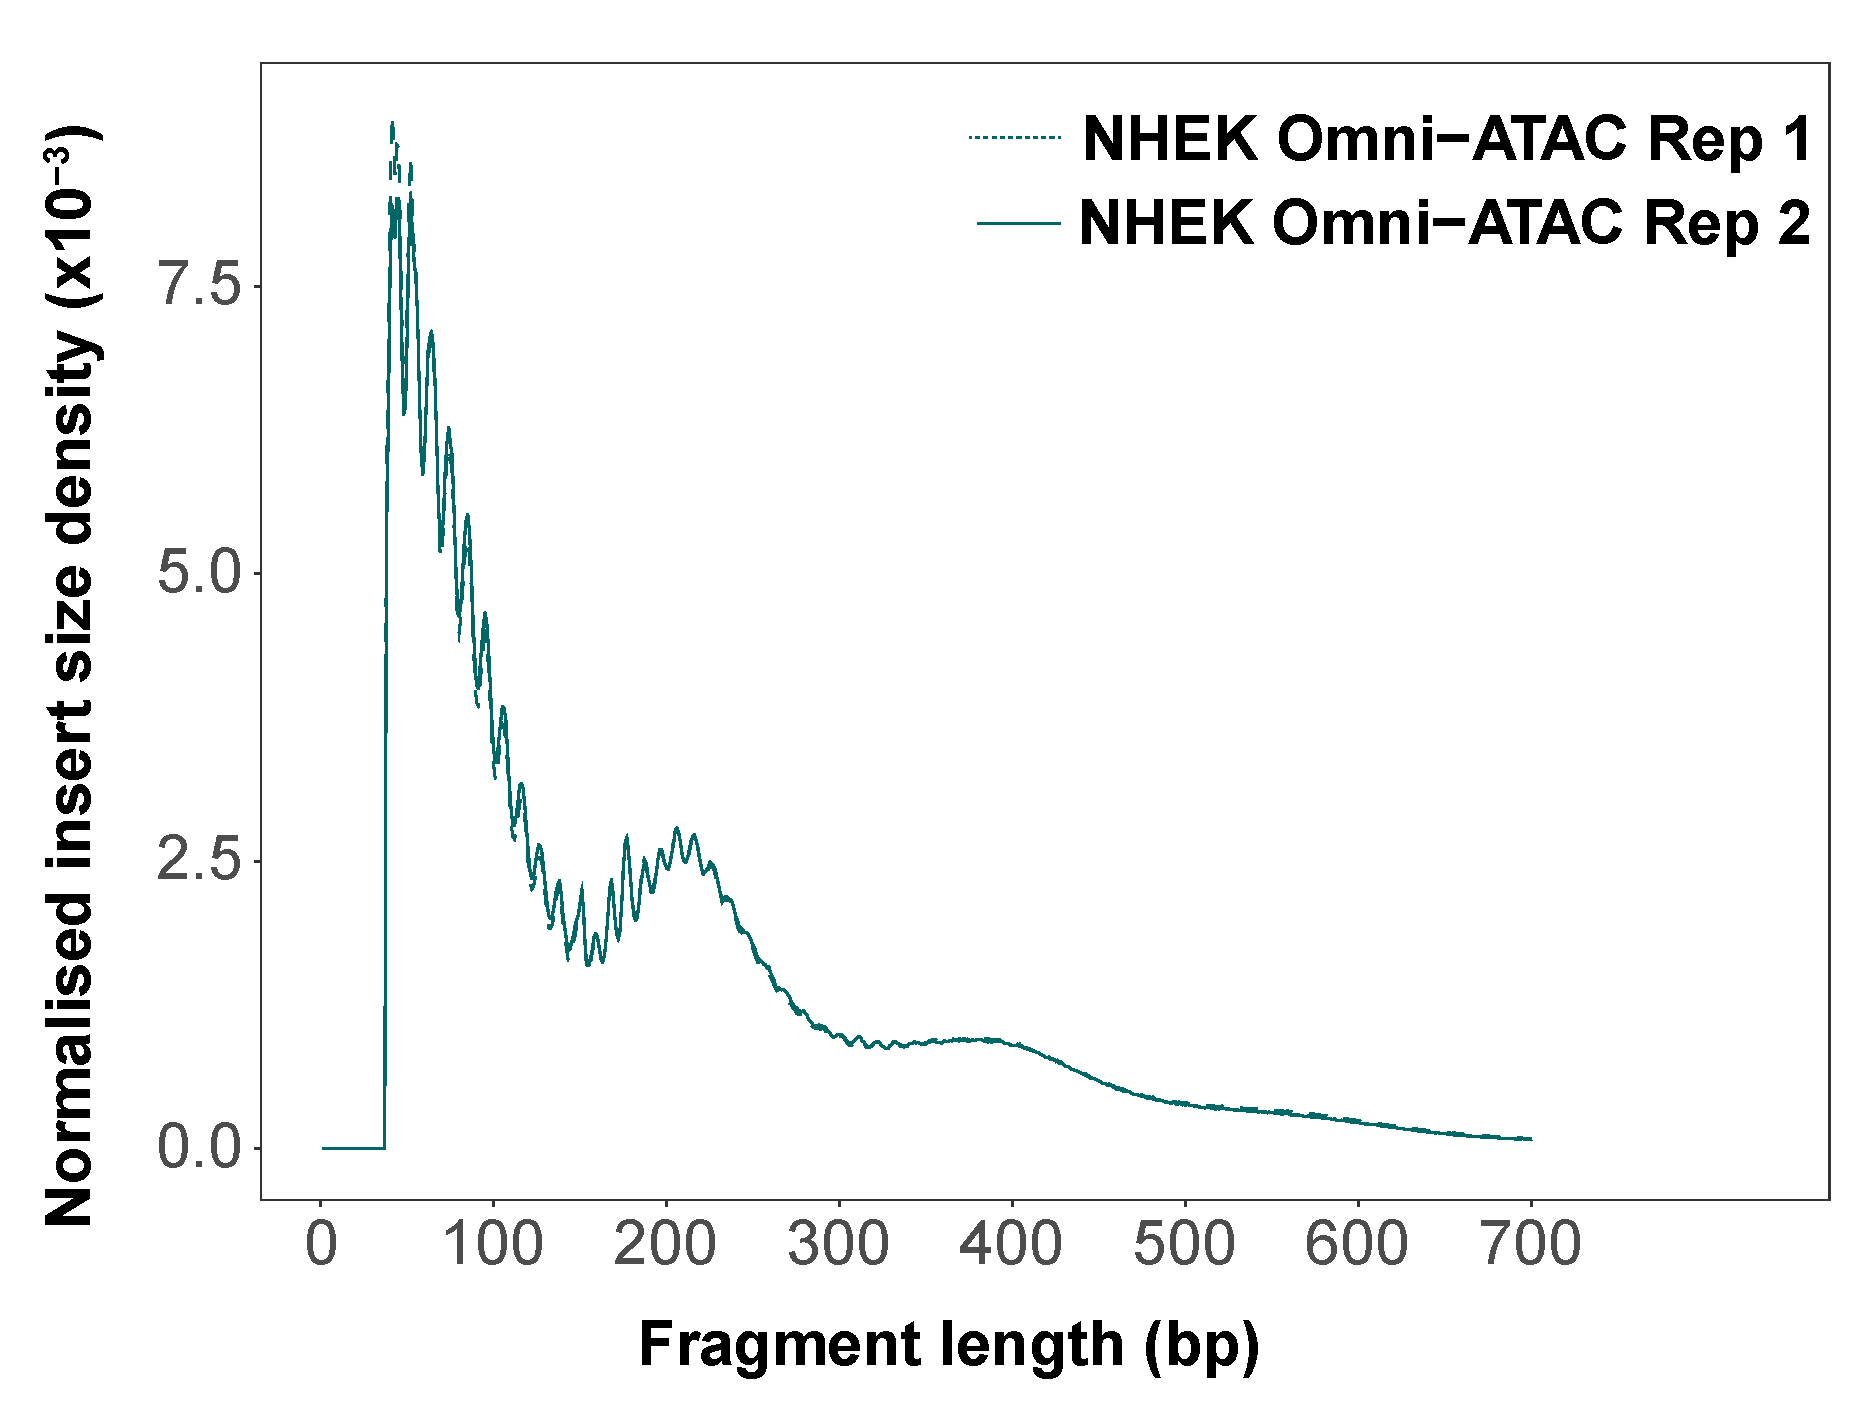
\includegraphics[width=\textwidth]{./Results1/pdfs/ATAC_NHEK_Omni_ATAC_fragment_size_distribution}
\caption{\textbf{}}
\end{subfigure}
\begin{subfigure}{0.5\textwidth}
\centering
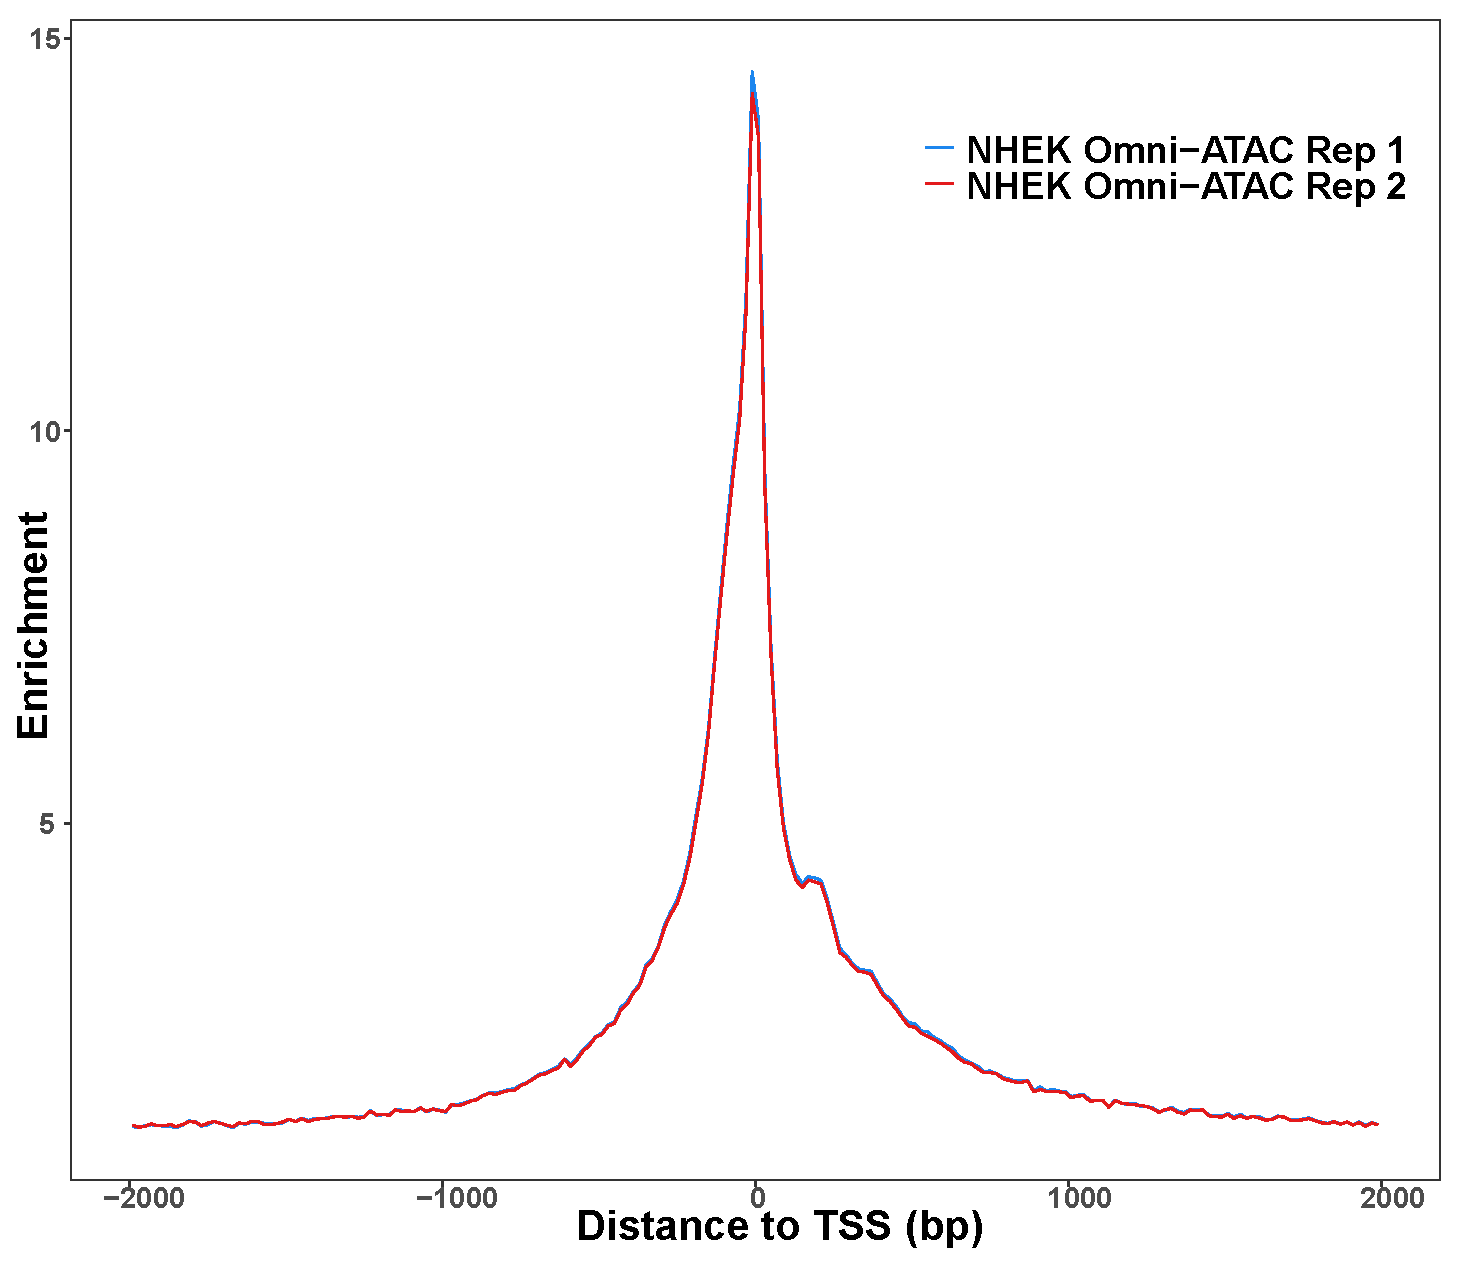
\includegraphics[width=\textwidth]{./Results1/pdfs/ATAC_skin_TSS_enrichment_NHEK_omni_ATAC}
\caption{\textbf{}} % to add text to the figure name
\end{subfigure}%
\caption[Quality control assessment of Fast-ATAC and Omni-ATAC in cultured NHEK]{\textbf{Quality control assessment of Fast-ATAC and Omni-ATAC in cultured NHEK.} Representation of the fragment sizes density distribution in NHEKs libraries generated using (A) ATAC 1, ATAC 2, Fast-ATAC or (B) Omni-ATAC protocols. (C) Fold-enrichment of ATAC fragments across the Ensembl annotated TSS from two Omni-ATAC technical replicates. In (A) the results for one of the two replicates is shown.}
\label{figure:Skin_ATAC1__ATAC2_Fast_ATAC_Omni_ATAC_QC_assessment}
\end{figure} 


At the end of the experimental work of this thesis, a new protocol called Omni-ATAC was published \parencite{Corces2017}. Omni-ATAC was a protocol suitable for every cell type, in contrast to ATAC 1 and Fast-ATAC, which were optimised for hematopoietic cells \parencite{Buenrostro2013,Corces2016}. Performance of this protocol in 50,000 viable NHEKs in suspension yielded the expected fragment size distribution for sequenced fragments, with the greatest abundance for NFF followed by mono and di-nucleosome fragments (Figure \ref{figure:PS02_skin_ATAC_QC_assessment}B). Moreover, high TSS enrichment values (approximately 15 fold change) were observed for the two replicates (Figure \ref{figure:PS02_skin_ATAC_QC_assessment}C). When performing overlap between the Omni-ATAC sample peaks filtered based on low stringency p-value (p-value=0.01) and the ENCODE DHSs from 125 cell types, the highest percentage of overlap (approximately 55\%) was observed for NHEKs (Figure \ref{figure:ATAC_skin_ENCODE_overlap_and_tracks}A). In contrast, the same analysis using peaks from the NHEKs libraries generated with ATAC 1, ATAC 2 and Fast-ATAC protocols only showed 20\% or less overlap with the ENCODE DHS data of the same cell type, supporting the higher quality and specificity of Omni-ATAC accessible regions in keratinocytes, even at a very low p-value filtering. The differences in the quality of ATAC signal between Omni-ATAC and the prior ATAC protocols was clearly observed at the keratin (\textit{KRT}) genes (main components of keratinocyte cytoskeleton) in chr17, where Omni-ATAC showed the lowest background noise, the highest signal intensity and the greatest number of high quality peaks (Figure \ref{figure:ATAC_skin_ENCODE_overlap_and_tracks}B). 

\begin{figure}[H]
\centering
\begin{subfigure}{0.40\textwidth}
\centering
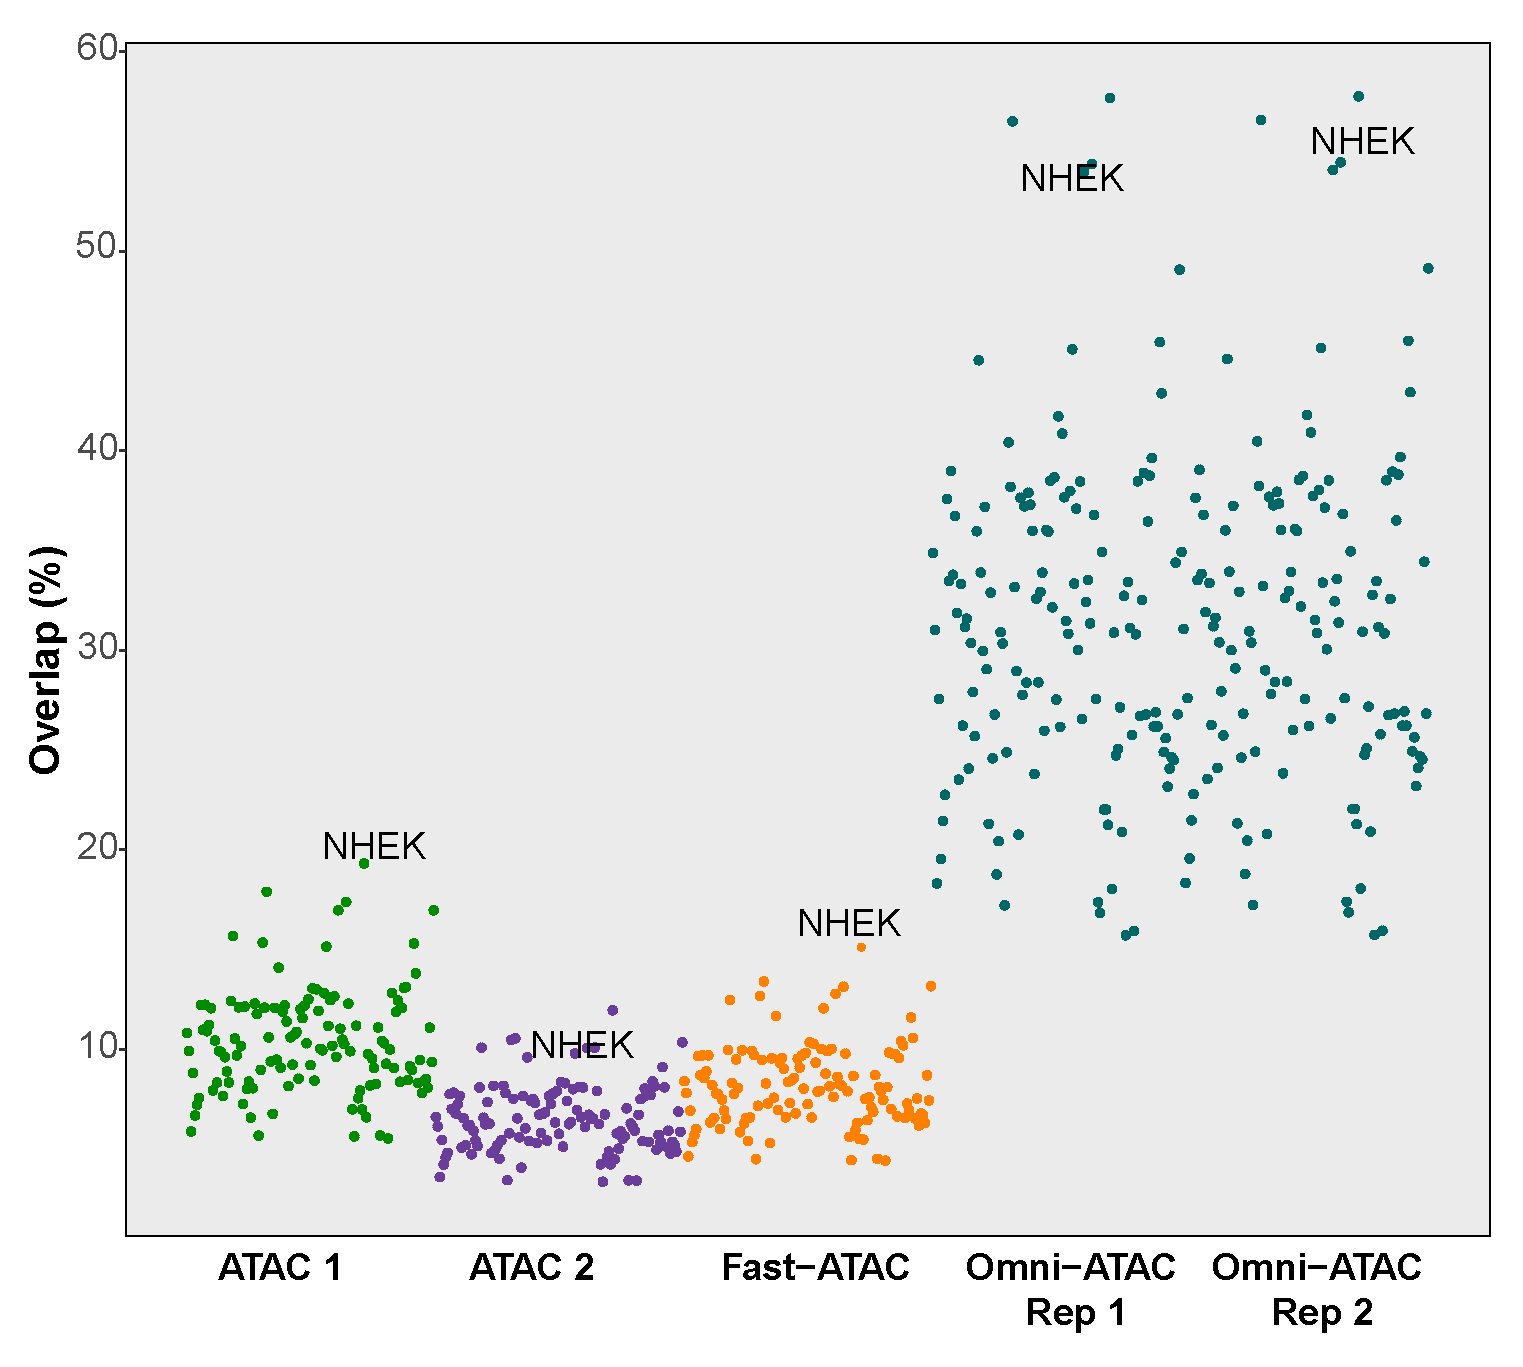
\includegraphics[width=\textwidth]{./Results1/pdfs/ENCODE_125_cell_types_overlap_FAST_ATAC_Omni_ATAC_pval_2}
\caption{\textbf{}}
% The percentage sign indicated that the other subfig goes side by side
\end{subfigure}
\begin{subfigure}{0.65\textwidth}
\centering
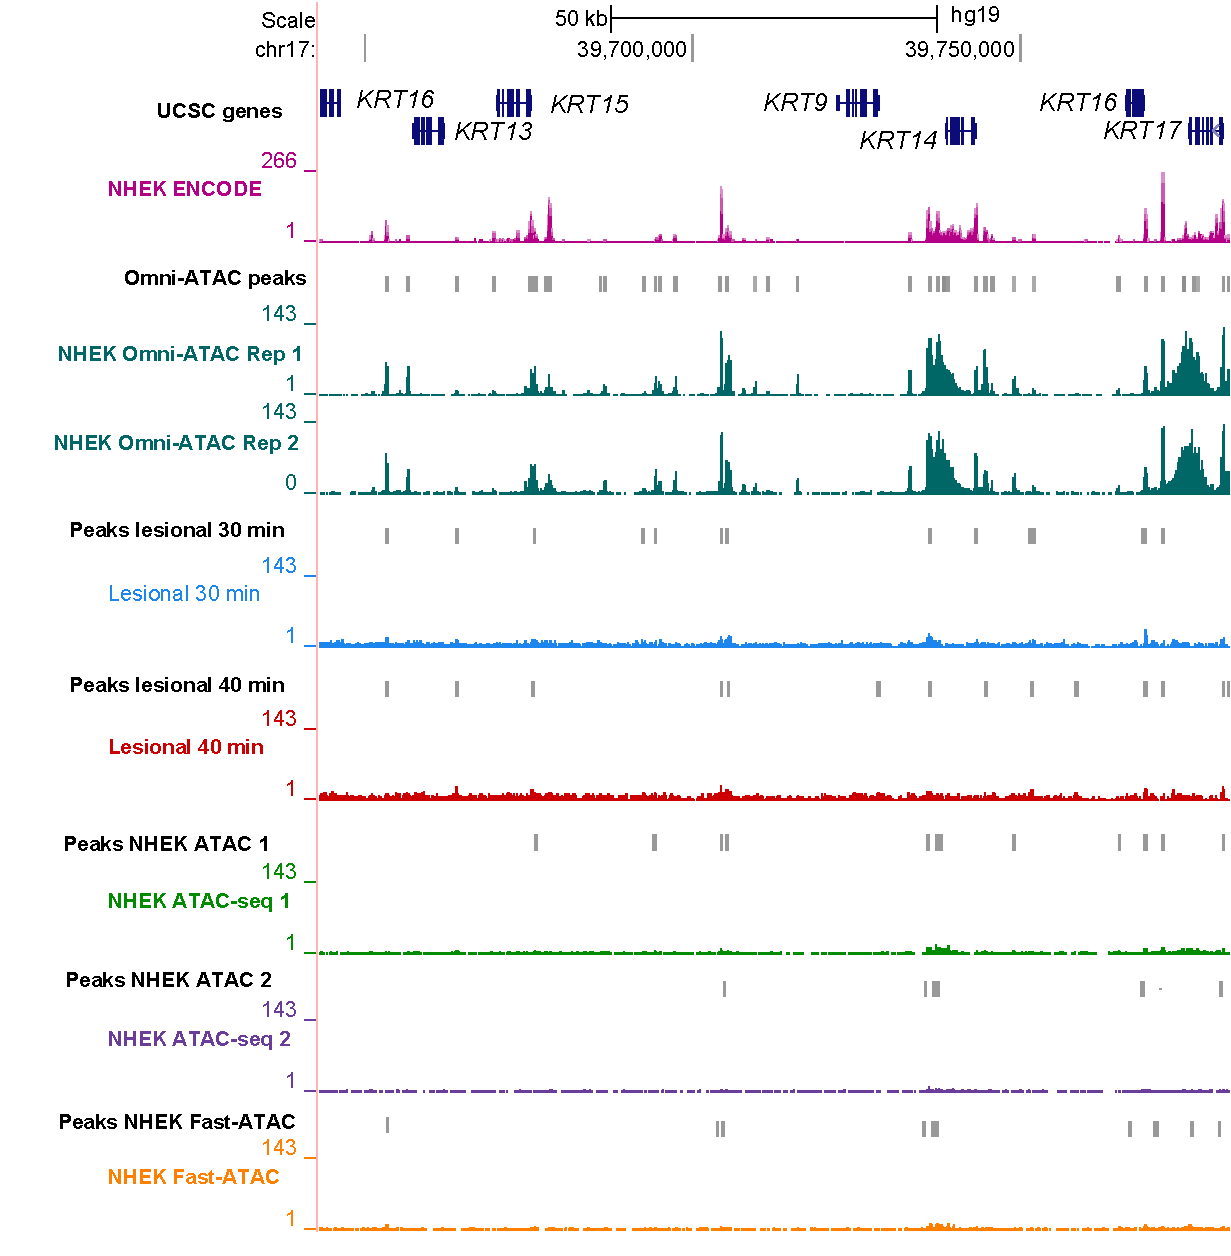
\includegraphics[width=\textwidth]{./Results1/pdfs/ATAC_skin_all_tracks_KRT}
\caption{\textbf{}}
\end{subfigure}
\caption[Comparison of 4 different ATAC protocols applied to psoriasis and/or healthy keratinocytes and NHEKs cells with published ENCODE DNase-seq data.]{\textbf{Comparison of 4 different ATAC protocols applied to psoriasis and/or healthy keratinocytes and NHEKs cells with published ENCODE DNase-seq data.} (A) Enrichment (\% of overlap) of observed peaks called in each ATAC sample (using low stringent p-value) with open DHS chromatin regions in 125 ENCODE cell types. (B) UCSC Genome Browser track showing open chromatin at the chr17 keratin (KRT) family gene locus for different ATAC protocols with the normalised ATAC read density (y-axis) shown.}
\label{figure:ATAC_skin_ENCODE_overlap_and_tracks}
\end{figure} 
\smallskip

 %Overall, this data was consistent with Corces \textit{et al.}, 2017, where consistent successful results in NHEKs were shown, and it encourages future testing of Omni-ATAC in keratinocytes from psoriasis patients biopsies processed through adherent assay to minimise the presence of dead cells.
	
\subsection{Effect of cryopreservation and fixation in the chromatin landscape of immune primary cells}
\label{Core}
\subsubsection{Experimental design and sample description}
As previously introduced, research using clinical samples represents a logistical challenge as immediate processing of freshly acquired cells may not be feasible. In the context of this thesis, two different possible approaches involving cryopreservation and fixation were of interest and a collaborative project to investigate these was established with High-Throughput Genomics at the WHG. The first approach was the cryopreservation of PBMCs in liquid nitrogen using DMSO followed by thawing, recovery and FACS isolation of the cell population of interest (Figure \ref{figure:Core_experimental_design}). Secondly, the performance of an optimised protocol developed by High-Throughput Genomics using DSP in scRNA-seq \parencite{Attar2018} was investigated as a short term preservation method for FACS-isolated relevant cell types.

In order to investigate the performance of these two strategies, blood from three healthy volunteers (Chapter \ref{ch:Mat} in Table \ref{tab:Summary_all_cohorts}) matched for sex and age (three females, mean age 25.6 years old) was processed on different days to simulate the experimental design when using patient samples (experimental design summarised in Figure \ref{figure:Core_experimental_design}). PBMCs were prepared from 90mL blood using a Ficoll gradient and CD14$^+$ monocytes and CD4$^+$ T cells were isolated by FACS, as detailed in Chapter \ref{ch:Mat}. ATAC-seq was performed on 50,000 CD14$^+$ monocytes and CD4$^+$ T cells, either freshly isolated or after fixation with DPS, stored at 4{$^\circ$}C for 24h and then processed for ATAC-seq (Figure \ref{figure:Core_experimental_design} Day 1, ATAC-seq fresh and ATAC-seq fixed, respectively). 

\begin{landscape}
\begin{figure}[H]
\centering
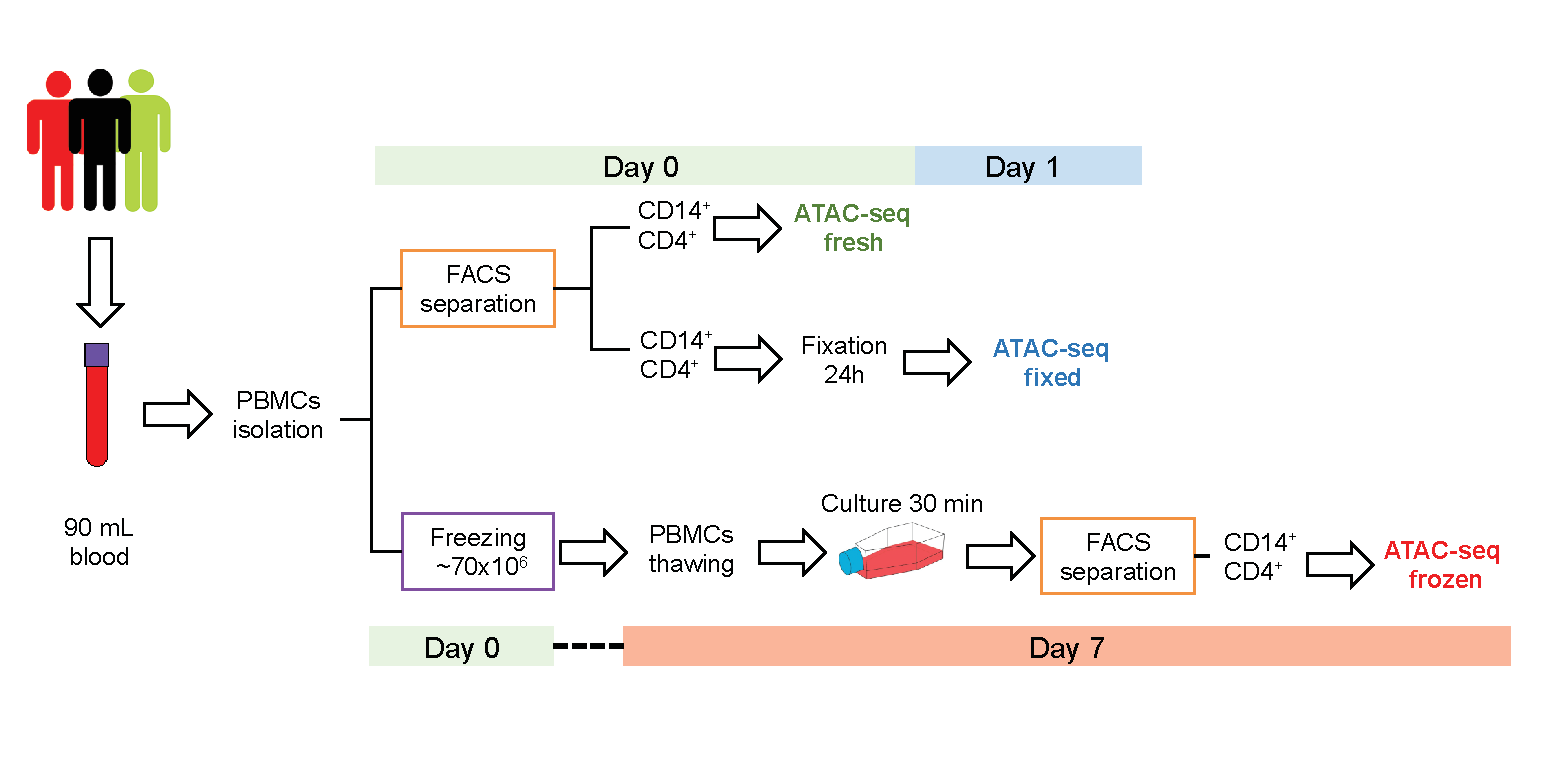
\includegraphics[width=1.2\textwidth]{./Results1/pdfs/Chapter3_core_experimental_design}
\caption[Experimental design to assess the impact of cryopreservation and fixation in the chromatin accessibility of immune primary cells.]{\textbf{Experimental design to assess the impact of cryopreservation and fixation in the chromatin accessibility of immune primary cells.} Three healthy control individuals were recruited on different days, PBMCs were isolated and freshly isolated CD14$^+$ monocytes or CD4$^+$ T cells processed for ATAC-seq immediately (ATAC-seq fresh), after fixation with DPS (ATAC-seq fixed) or after cryopreservation of PBMCs (ATAC-seq frozen).}%Three healthy control individuals were recruited on different days and PBMCs were isolated from 90mL of blood (Day 0). on Day 0, a fraction of PBMCs were used for FACS staining and isolation of 50,000 CD14$^+$ and CD4$^+$, which were directly processed for ATAC-seq (ATAC-seq fresh). Also on Day 0, a 50,000 FACS-sorted CD14$^+$ and CD4$^+$ cells were fixed with DPS, stored at 4{$^\circ$}C for 24h and processed for ATAC-seq in Day 1 (ATAC-seq fixed). Lastly, on Day 0 a fraction of the PBMCs (70x10$^6$ million cells) were cryopreserved in DMSO and slow-cooling. On Day 7 of storage in liquid nitrogen, PBMCs were thawed, recovered in culture for 30 min and stained with FACS Abs to isolate 50,000 CD14$^+$ and CD4$^+$cell to perform ATAC-seq (ATAC-seq frozen).}
\label{figure:Core_experimental_design}
\end{figure}
\end{landscape}

To investigate the effect of cryopreservation and cell recovery in the chromatin landscape of primary immune cells, 70x10$^6$ million PBMCs were cryopreserved with DMSO on the day of collection and stored in liquid nitrogen followed by thawing and recovery in culture for approximately 30 min (as detailed in Chapter \ref{ch:Mat}). After recovery, CD14$^+$ monocytes and CD4$^+$ T cells were isolated from the PBMCs by FACS and then ATAC-seq was performed (Figure \ref{figure:Core_experimental_design} Day 7, ATAC-seq frozen). Altogether, for each volunteer, three matched ATAC-seq libraries were generated in two different cell populations: ATAC-seq fresh, ATAC-seq fixed and ATAC-seq frozen.

\subsubsection{Assessment of the chromatin structure preservation in the different conditions}

All samples from each of the two cell types had more than 15 million reads, which has previously been shown as the minimum for successful ATAC-seq analysis and peak calling (Figure \ref{figure:Core_ATAC_all_conditions_total_reads}). The median number of reads across the fresh, frozen and fixed were more similar for CD14$^+$ monocytes (58.6, 64.2 and 39.6 million reads, respectively) than in the CD4$^+$ samples, where the frozen and fixed presented lower median total reads compared to the controls (43.8, 32.9 and 28.8 million reads respectively)(Figure \ref{figure:Core_ATAC_all_conditions_total_reads}A and B).

\begin{figure}[htbp]
\centering
\begin{subfigure}{0.5\textwidth}
\centering
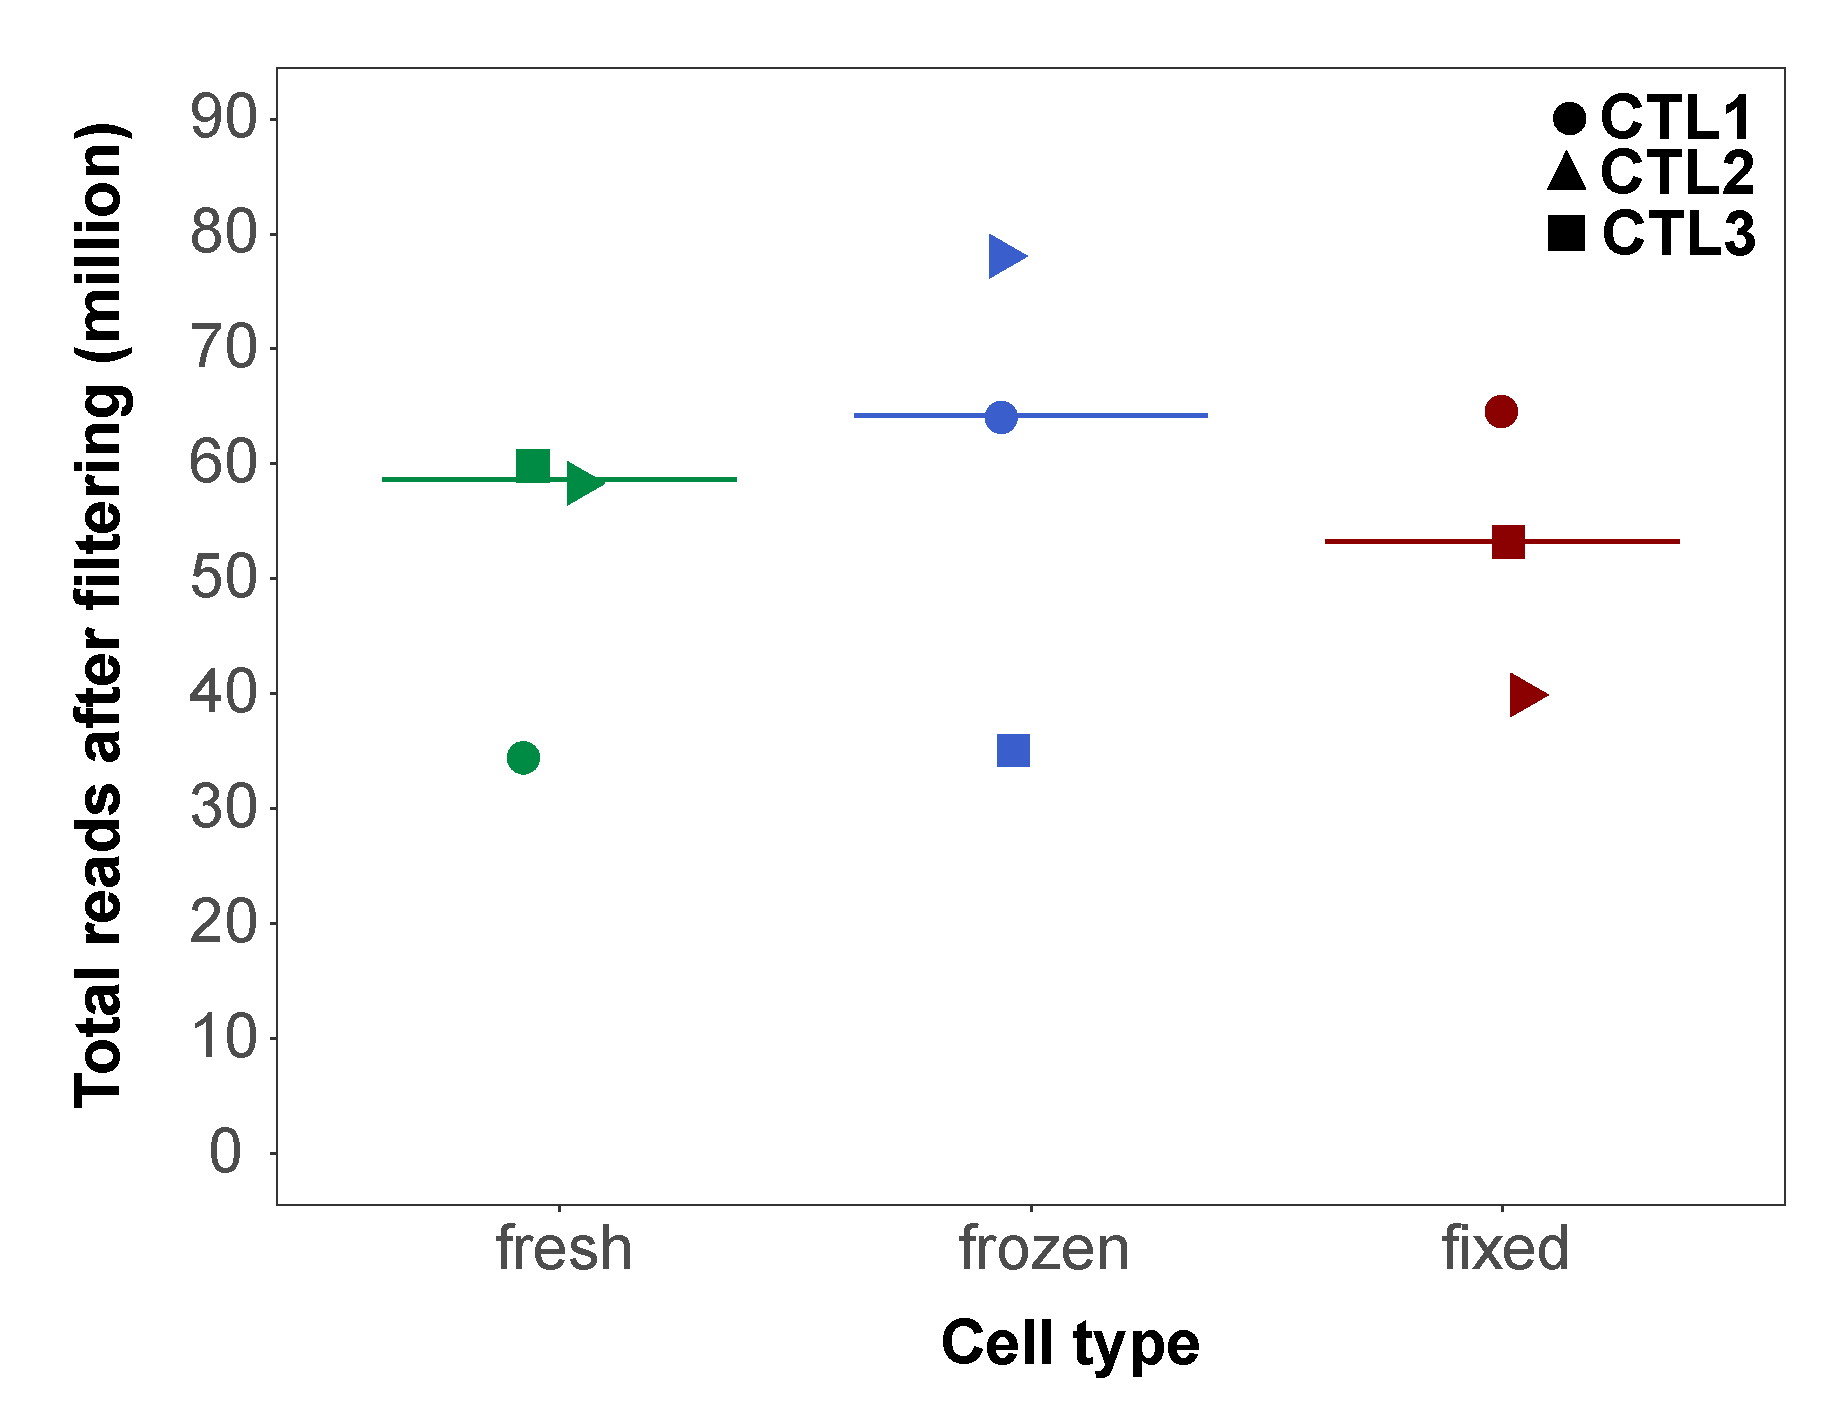
\includegraphics[width=\textwidth]{./Results1/pdfs/Core_ATAC_CD14_fresh_frozen_fixed_filtered_total_reads}
\caption{\textbf{}}
% The percentage sign indicated that the other subfig goes side by side
\end{subfigure}%
\begin{subfigure}{0.5\textwidth}
\centering
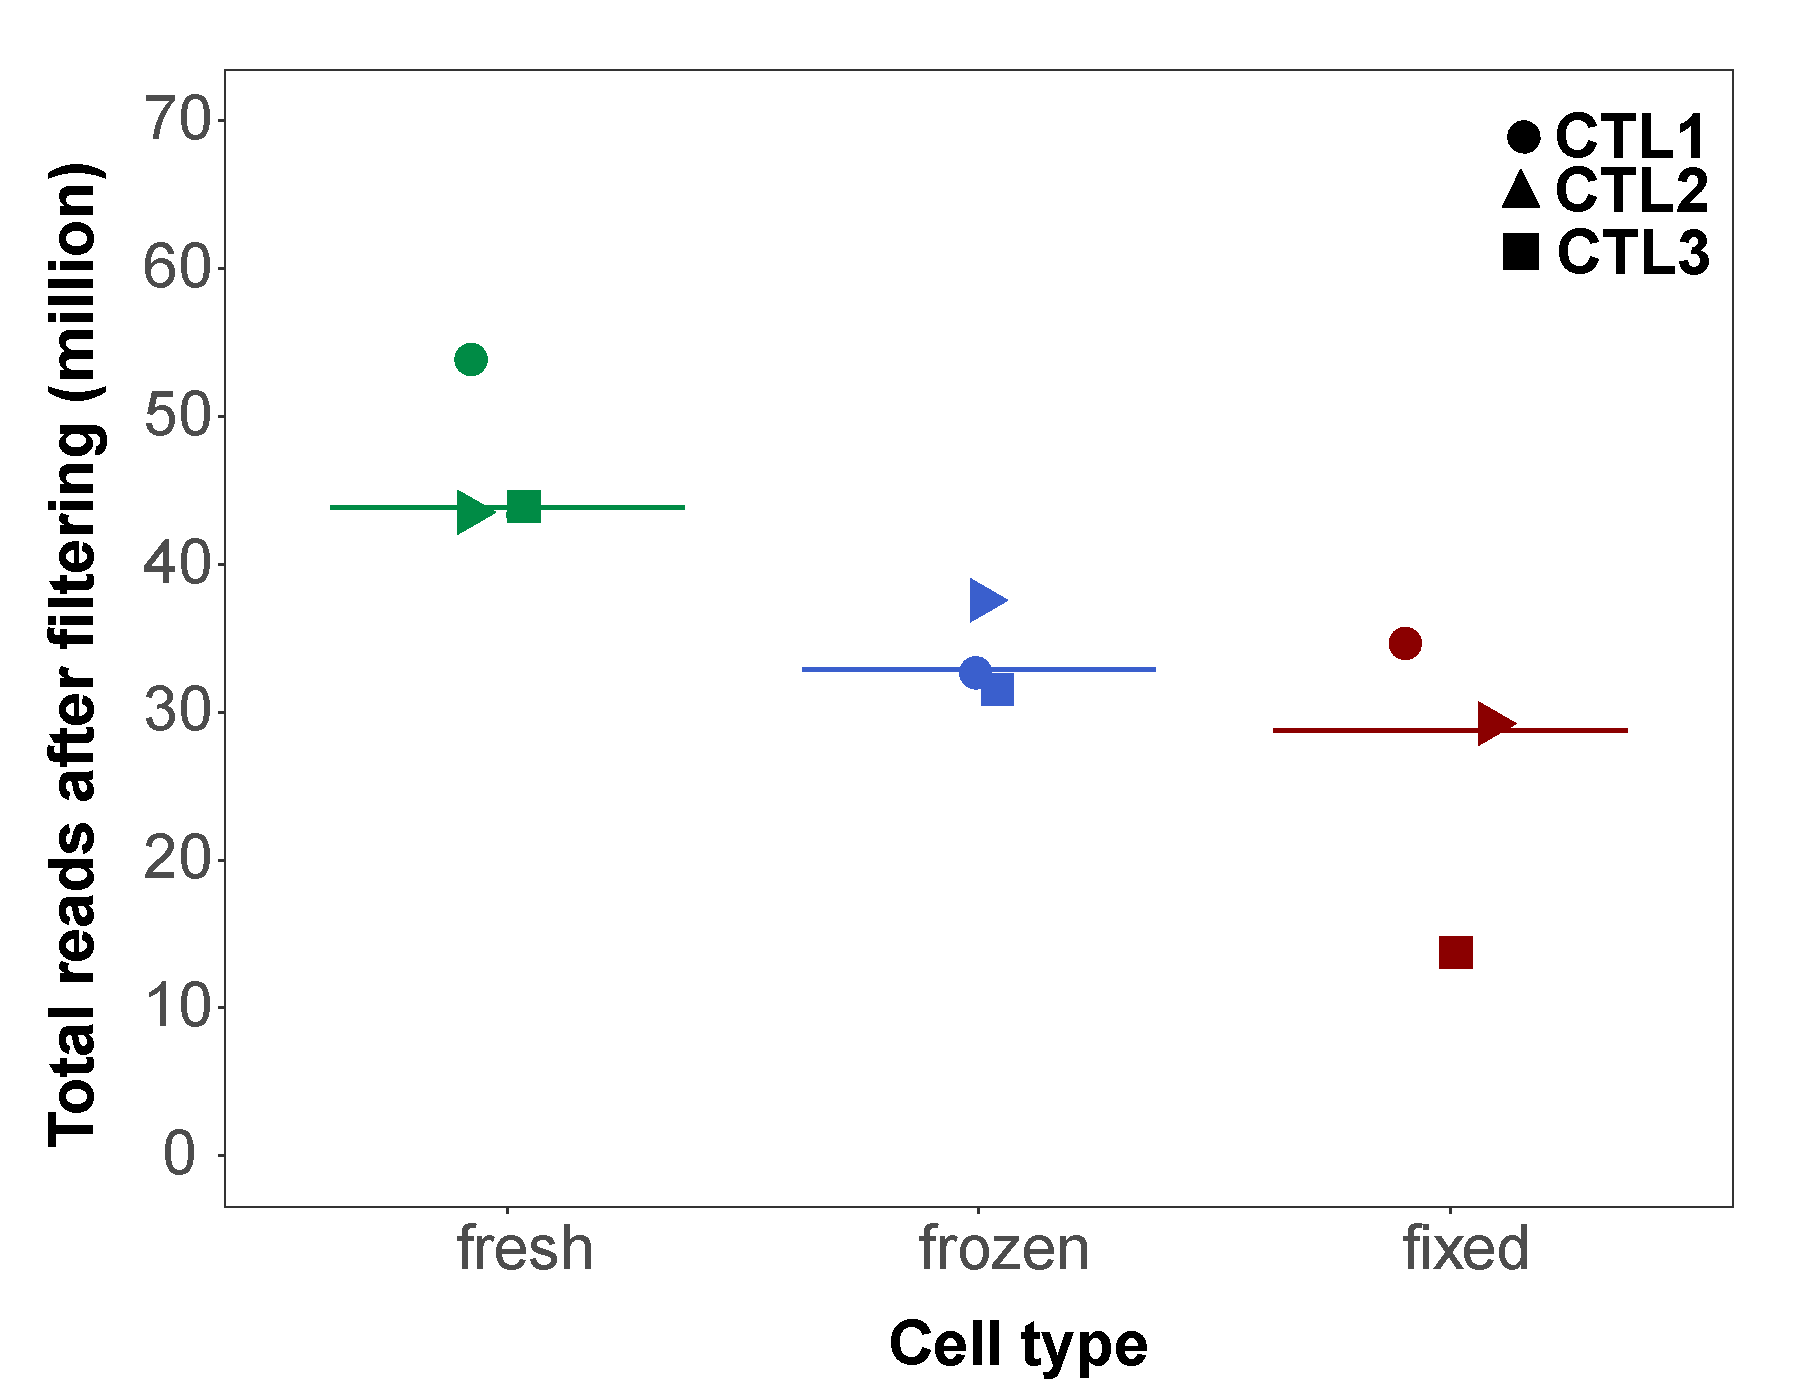
\includegraphics[width=\textwidth]{./Results1/pdfs/Core_ATAC_CD4_fresh_frozen_fixed_filtered_total_reads}
\caption{\textbf{}}
\end{subfigure}
\caption[Total number of ATAC-seq reads for the fresh, frozen and fixed CD14$^+$ monocytes and CD4$^+$ samples for three volunteers (CTL1-3).]{\textbf{Total number of ATAC-seq reads for the fresh, frozen and fixed CD14$^+$ monocytes and CD4$^+$ samples for three volunteers (CTL1-3).} Representation of million reads after filtering for the fresh, fixed and frozen ATAC-seq libraries in (A) CD14$^+$ monocytes and (B) CD4$^+$ cells.}
\label{figure:Core_ATAC_all_conditions_total_reads}
\end{figure} 

The ATAC-seq signal-to-noise ratios across the TSS showed a similar median for the fresh and fixed CD14$^+$ monocytes libraries (17.4 and 16.5 fold-enrichment, respectively) and was higher for the frozen samples (26.3 fold-enrichment)(Table \ref{tab:Core_ATAC_TSS_summary_table}). The median TSS enrichments in the frozen and fixed CD4$^+$ samples were considerably higher (16.1 and 14.3 fold-enrichment, respectively) than the fresh samples (5.6), which were borderline for the ENCODE recommended threshold. For one volunteer (CTL1) the fixed samples of both cell types showed considerably lower TSS enrichment (2.5 and 7.9, respectively) compared to the other fixed samples (Table \ref{tab:Core_ATAC_TSS_summary_table}). As expected, the fragment size distribution profiles of the fresh and frozen samples for both cell types were very similar, showing appropriate relative abundance of NFF and NBF corresponding to mono-, di-, tri- and tetra-nucleosomes (Figure \ref{figure:Core_ATAC_all_fragment_size_distribution}A and B green and blue lines). Conversely, fixed samples showed differences in the fragment size distribution profiles, where for both cell types a fraction of NFF was absent in CTL2 and CTL3 and extremely low in CTL1 (Figure \ref{figure:Core_ATAC_all_fragment_size_distribution} red lines). 


Chromatin structure across and within the TSS was then investigated following Scharer and colleagues approach \parencite{Scharer2016}. The nucleosome-free fragments ($<$150bp) from all the samples showed a single peak of enrichment at the nucleosome-depleted TSS position, with CD4$^+$ fresh samples presenting the lowest enrichment (Figure \ref{figure:Core_ATAC_intra_dinucleosome_tss_enrichment}A and C).

\begin{figure}[htbp]
\centering
\begin{subfigure}{0.5\textwidth}
\centering
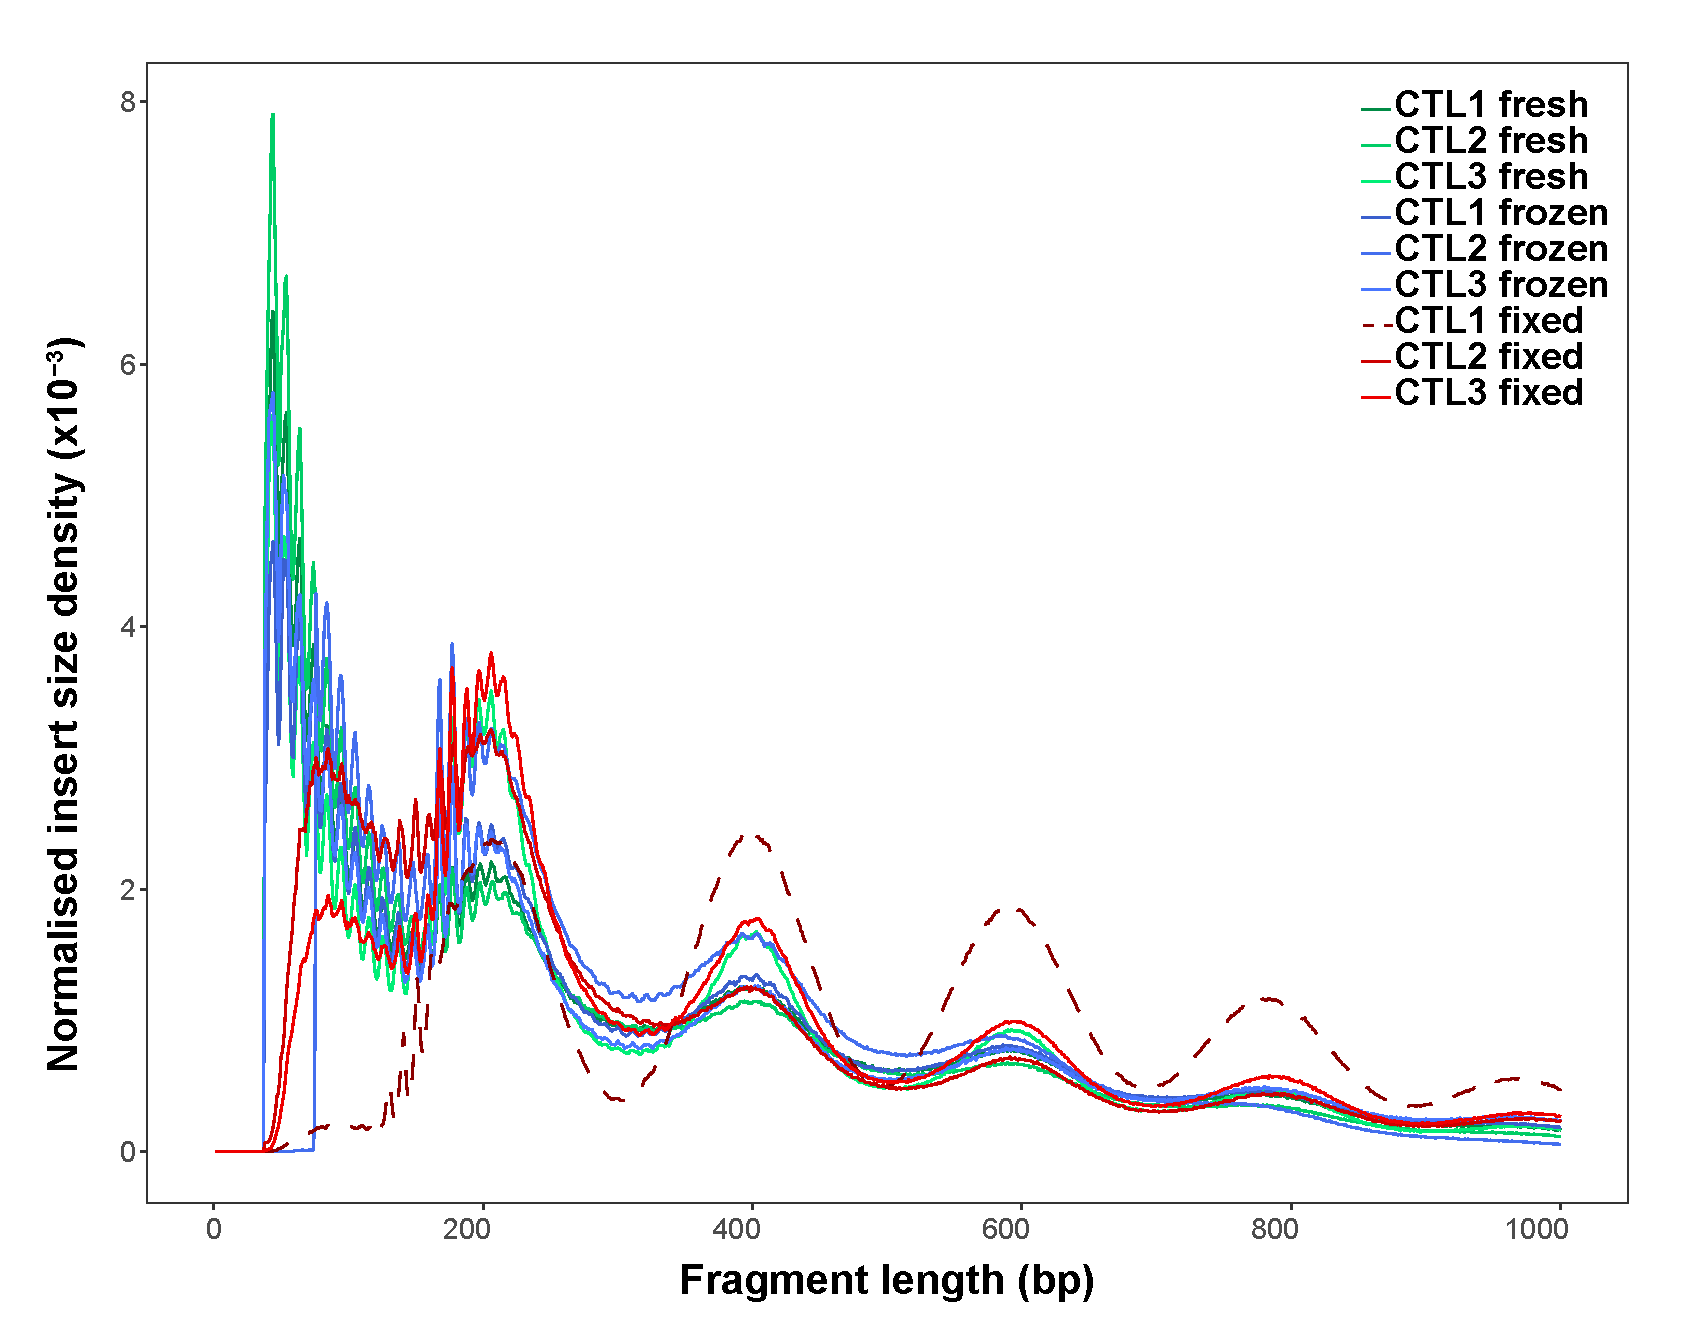
\includegraphics[width=\textwidth]{./Results1/pdfs/Core_ATAC_CD14_fresh_frozen_fixed_frag_size_distribution}
\caption{\textbf{}}
% The percentage sign indicated that the other subfig goes side by side
\end{subfigure}%
\begin{subfigure}{0.5\textwidth}
\centering
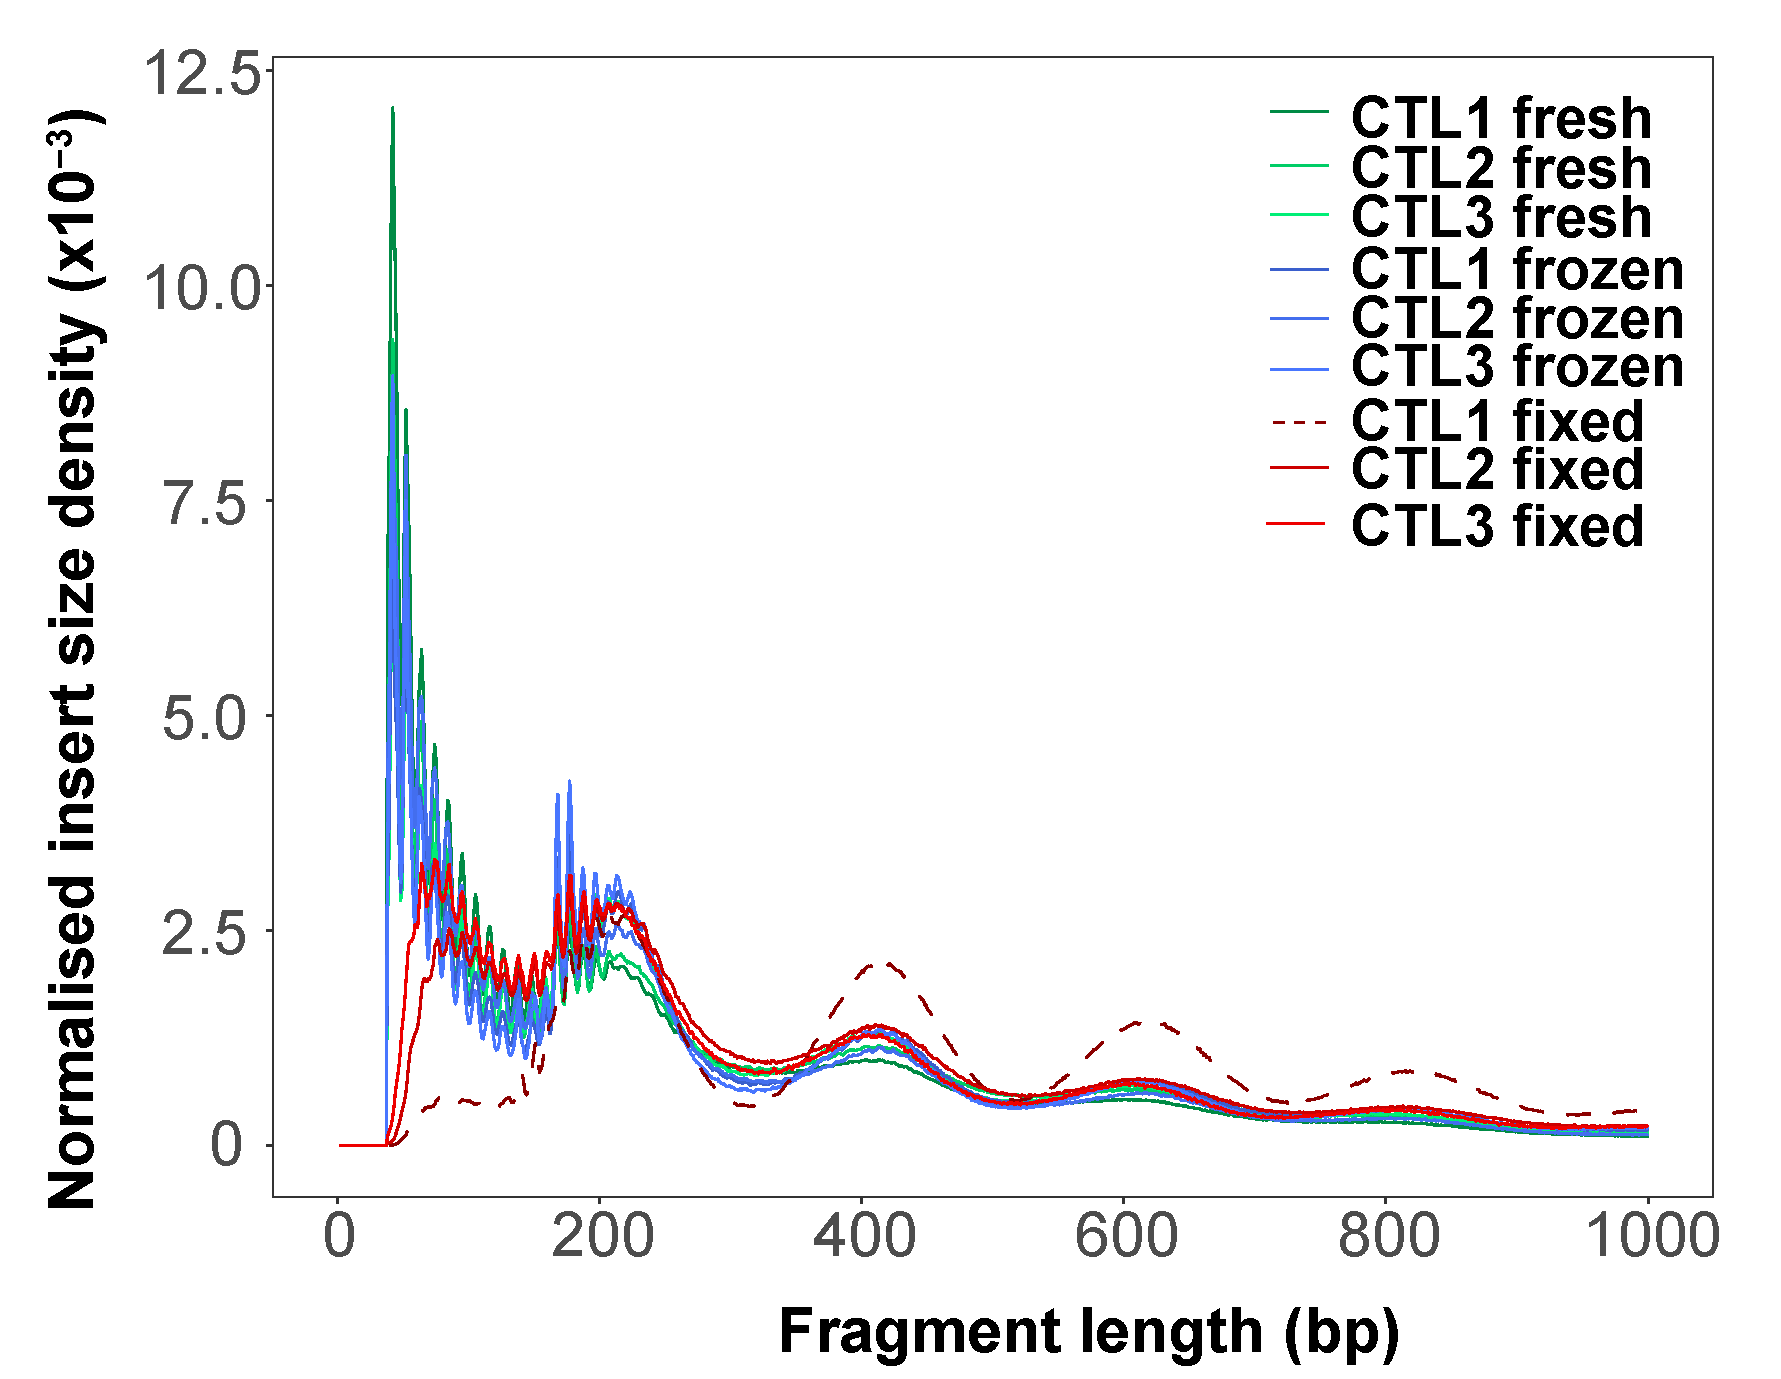
\includegraphics[width=\textwidth]{./Results1/pdfs/Core_ATAC_CD4_fresh_frozen_fixed_frag_size_distribution}
\caption{\textbf{}}
\end{subfigure}
\caption[Fragment size density distribution for ATAC-seq fresh, fixed and frozen in CD14$^+$ monocytes and CD4$^+$ cells.]{\textbf{Fragment size density distribution for ATAC-seq fresh, fixed and frozen in CD14$^+$ monocytes and CD4$^+$ cells.} The distribution of ATAC-seq fragment lengths are illustrated for (A) CD14$^+$ monocytes and (B) CD4$^+$ cells and colour-coded by condition (fresh=green, frozen=blue and fixed=red).}
\label{figure:Core_ATAC_all_fragment_size_distribution}
\end{figure} 


The pattern of enrichment of di-nucleosome fragments (ranging between 260 and 340bp) demonstrated in the majority of the samples periodicity in the TSS surroundings, with two peaks of enrichment mapping at the characteristic up-stream and down-stream positioned nucleosomes (Figure \ref{figure:Core_ATAC_intra_dinucleosome_tss_enrichment}B and D). Although fixation in CD14$^+$ and CD4$^+$ CTL1 samples drastically reduced the abundance of NFF, the ATAC-seq signal for the remaining ones was clearly enriched at TSS (Figure \ref{figure:Core_ATAC_intra_dinucleosome_tss_enrichment}A and C). Interestingly, despite fixed CD14$^+$ CTL1 having increased density of NBF (in this case di-, tri- and tetra-nucleosomes) loss of chromatin structure around the TSS suggested that nucleosomes may have been displaced from their original position, likely due to the fixative not cross-linking proteins to DNA, and therefore explaining this lack of enrichment (Figure \ref{figure:Core_ATAC_intra_dinucleosome_tss_enrichment}B). CD4$^+$ fresh samples showed comparatively low enrichment at the TSS for NFF and di-nucleosome fragments, consistent with the overall borderline signal-to-noise ratio of the samples (Figure \ref{figure:Core_ATAC_intra_dinucleosome_tss_enrichment}B and D and Table \ref{tab:Core_ATAC_TSS_summary_table}).


%This pattern of enrichment was weaker in the three fresh samples from CD4$^+$ and absent in the CTL1 CD14$^+$ fixed sample. The fresh CD4$^+$ samples also presented low enrichment for the nucleosome-free fragments in the TSS, similar to their overall TSS enrichment (Table \ref{tab:Core_ATAC_TSS_summary_table}) but still weakly identified the position of the two nucleosomes in the TSS surroundings, suggesting an overall preservation of the chromatin structure. 



\begin{figure}[htbp]
\centering
\begin{subfigure}[b]{0.45\textwidth}
\centering 
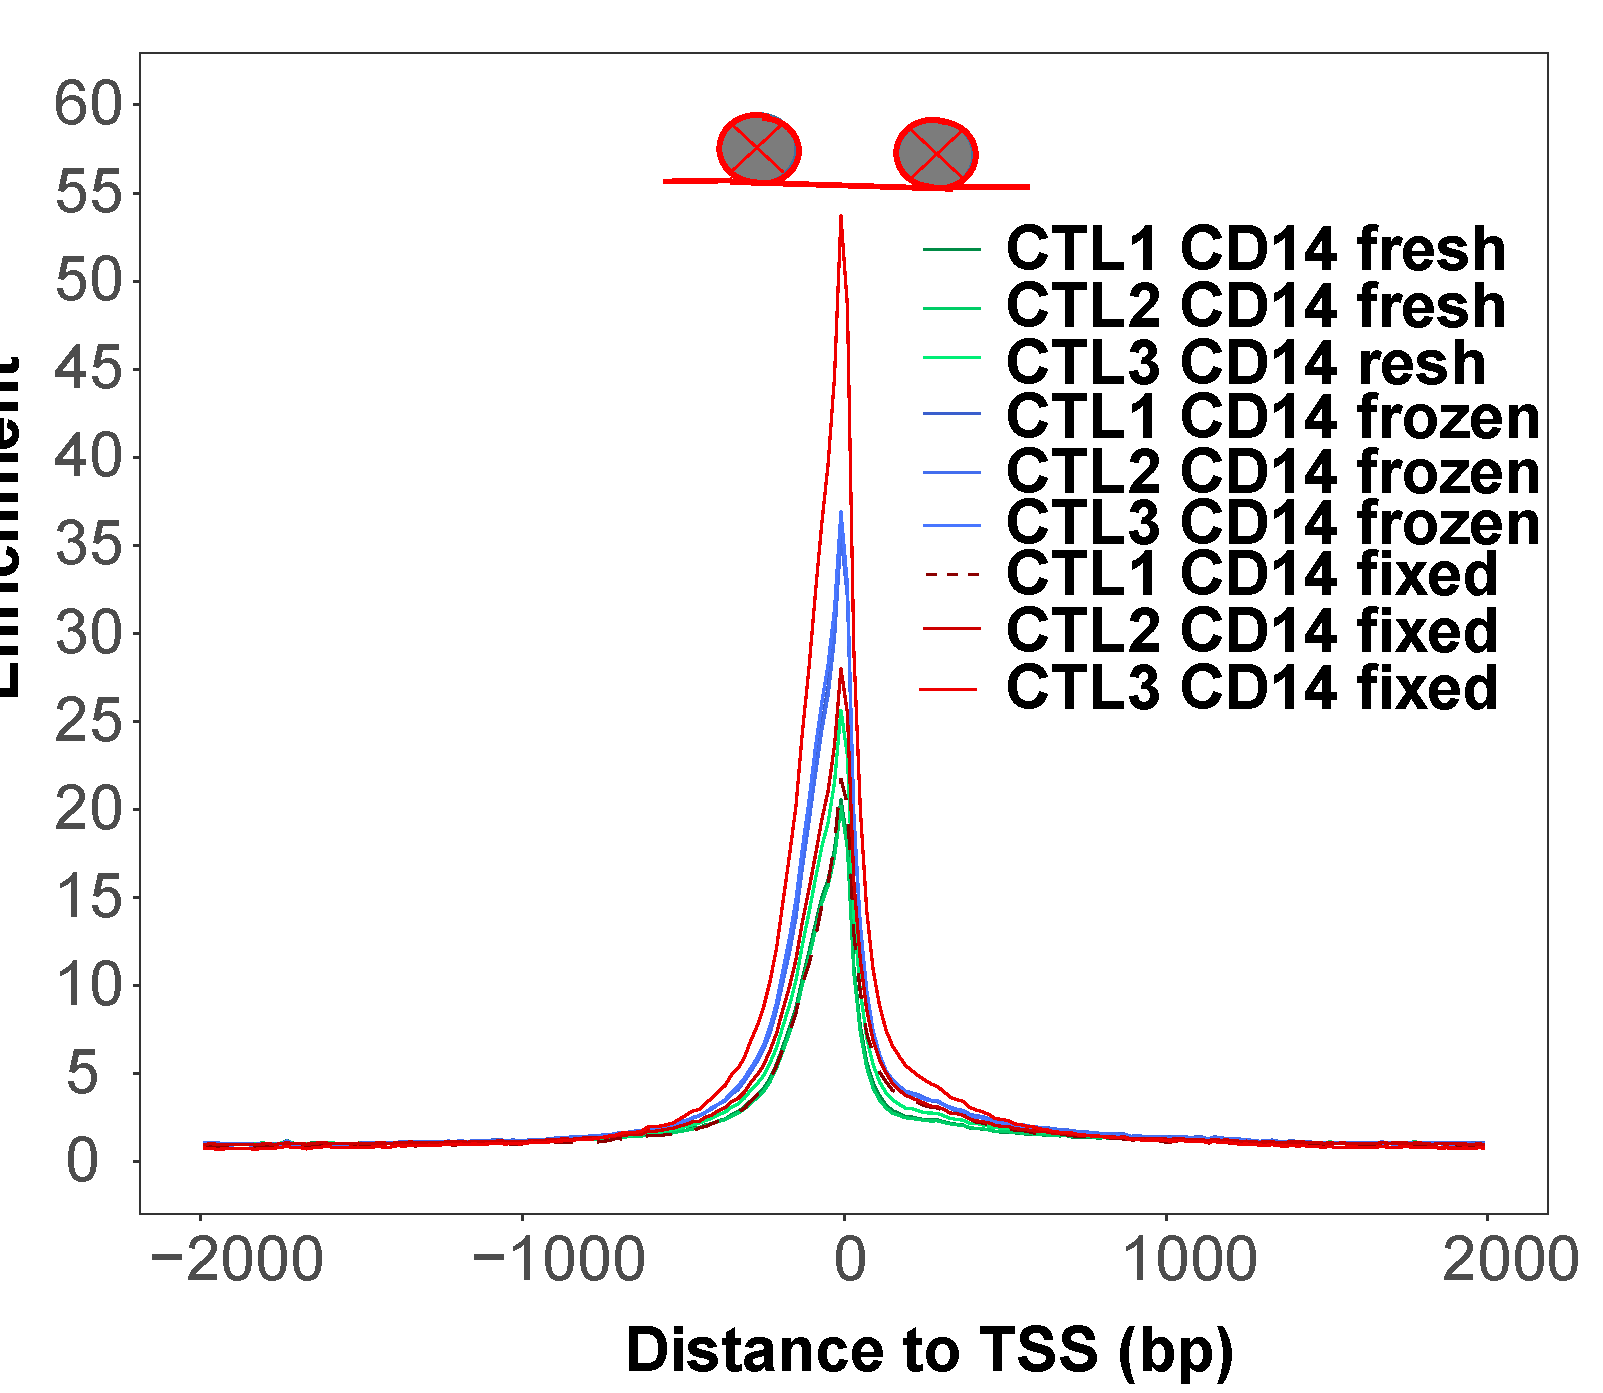
\includegraphics[width=\textwidth]{./Results1/pdfs/Core_ATAC_CD14_fresh_frozen_fixed_internucleosome_TSS}
\caption{}
\end{subfigure}
~
\begin{subfigure}[b]{0.45\textwidth}
\centering 
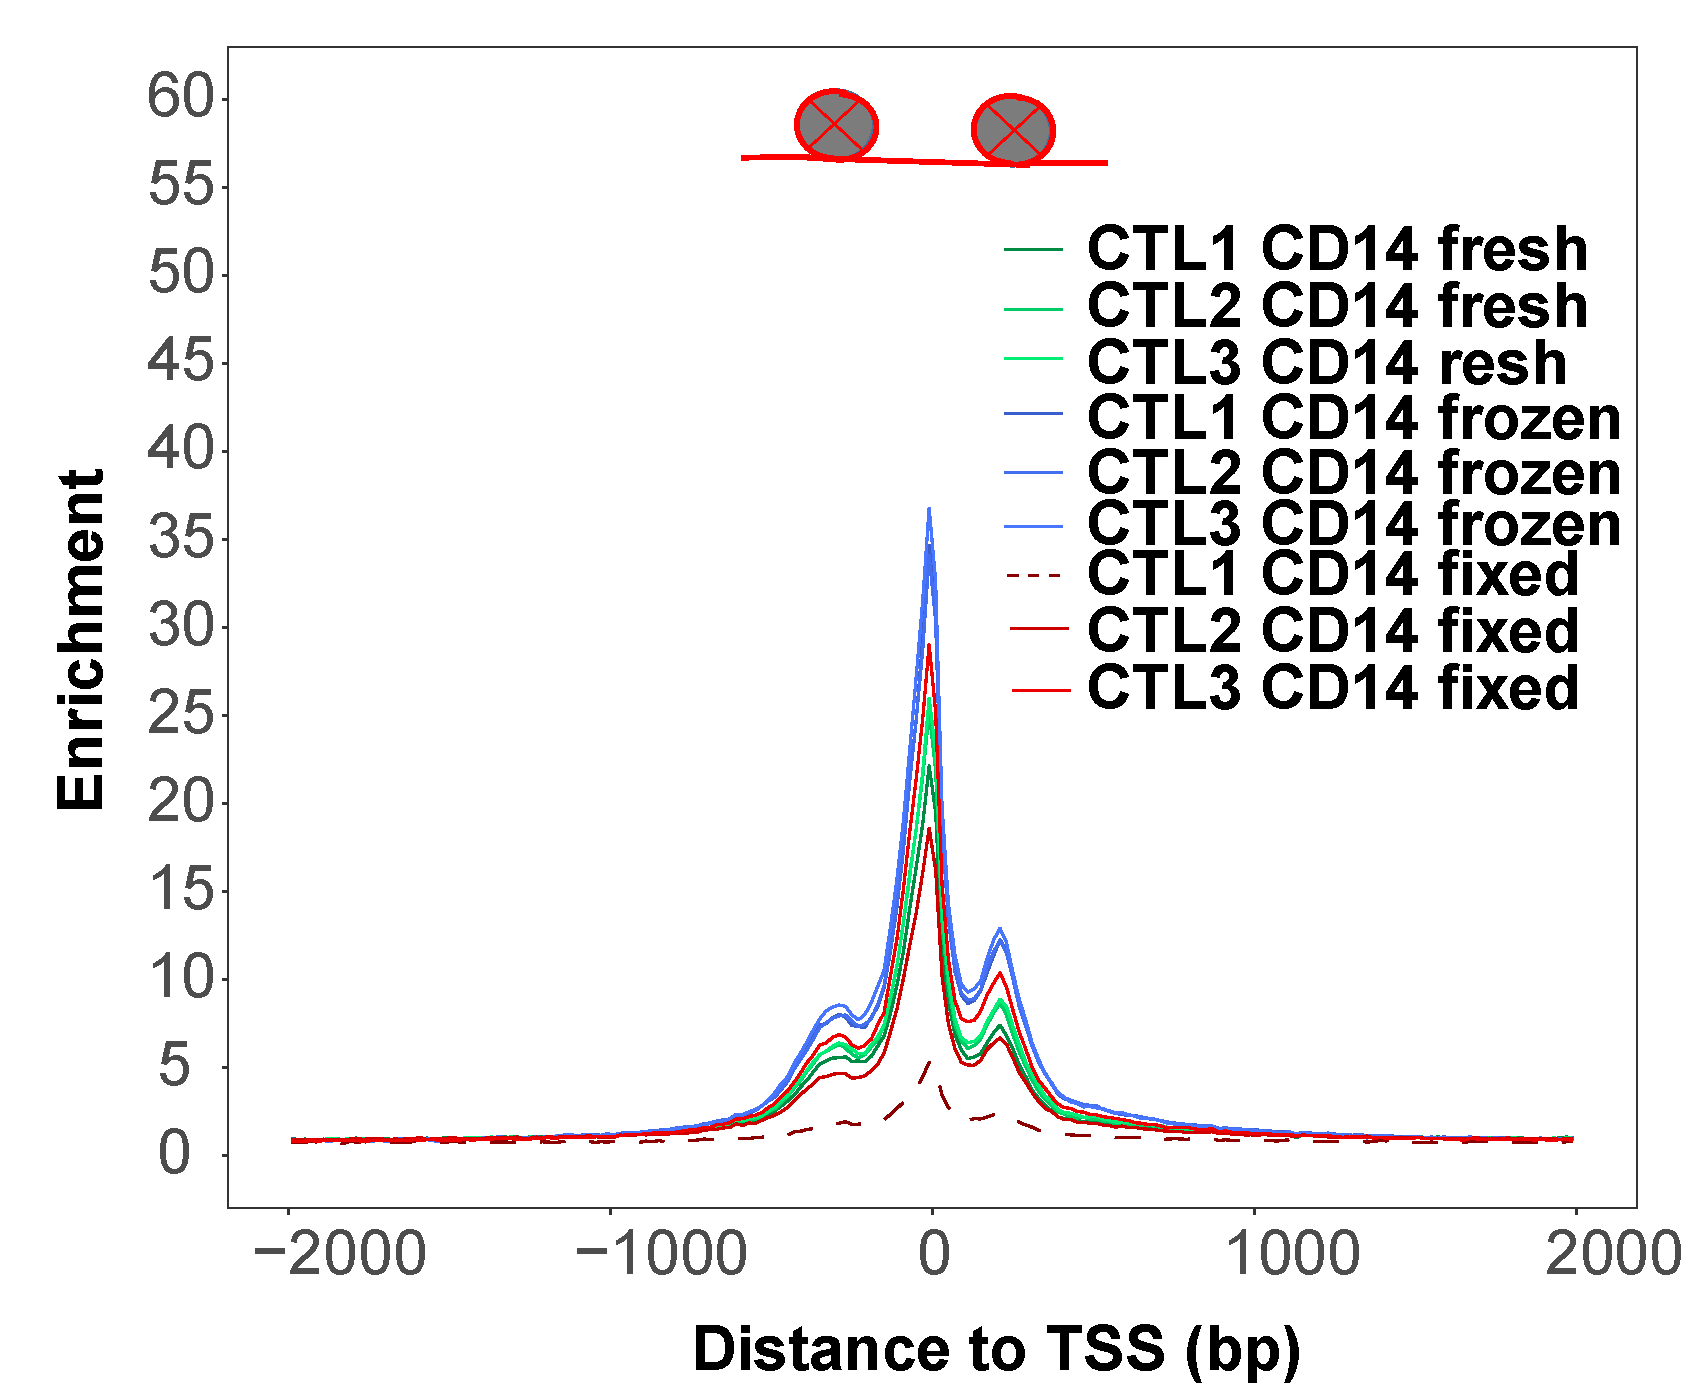
\includegraphics[width=\textwidth]{./Results1/pdfs/Core_ATAC_CD14_fresh_frozen_fixed_dinucleosome_TSS}
\caption{}
\end{subfigure}
~
\begin{subfigure}[b]{0.45\textwidth} 
%the [b] prevents offset in subcaptions
\centering
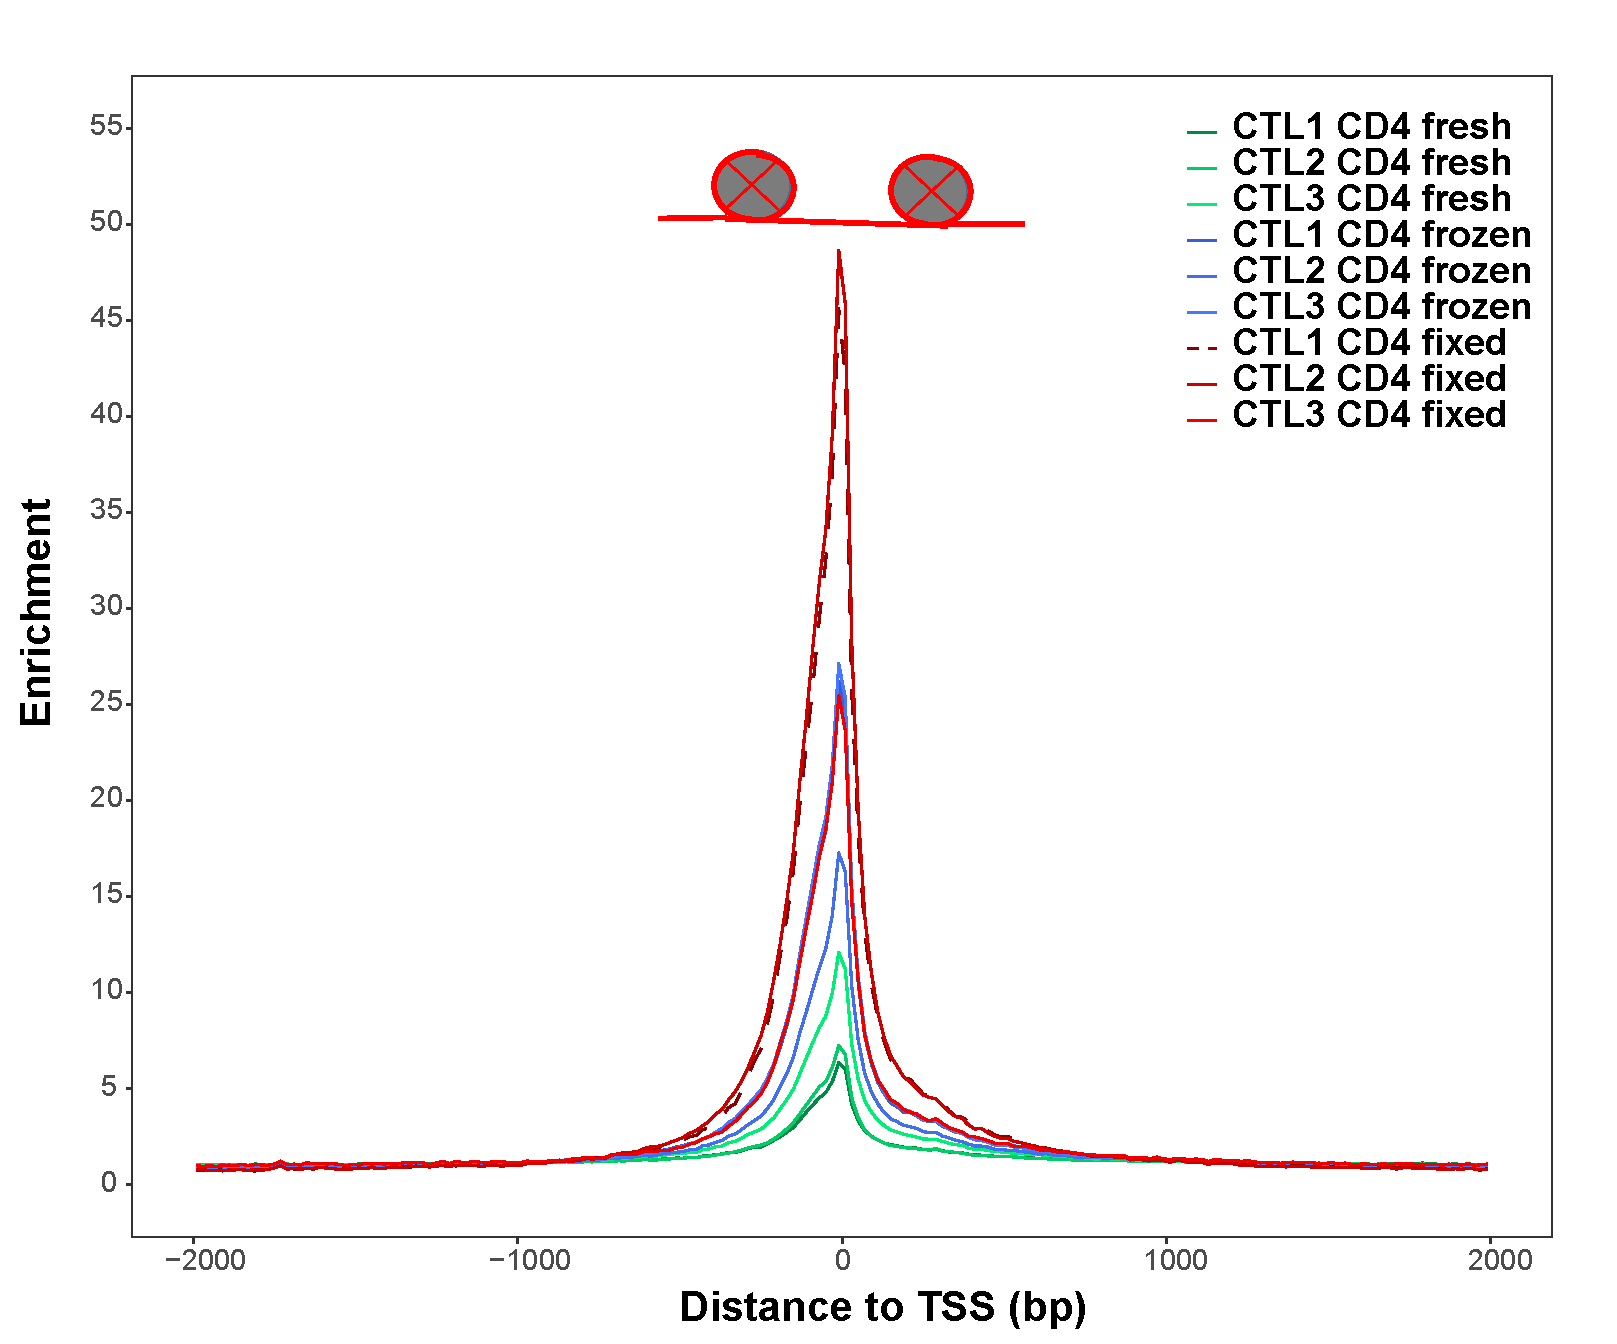
\includegraphics[width=\textwidth]{./Results1/pdfs/Core_ATAC_CD4_fresh_frozen_fixed_internucleosome_TSS}%
\caption{}
\end{subfigure}
\begin{subfigure}[b]{0.45\textwidth} 
%the [b] prevents offset in subcaptions
\centering
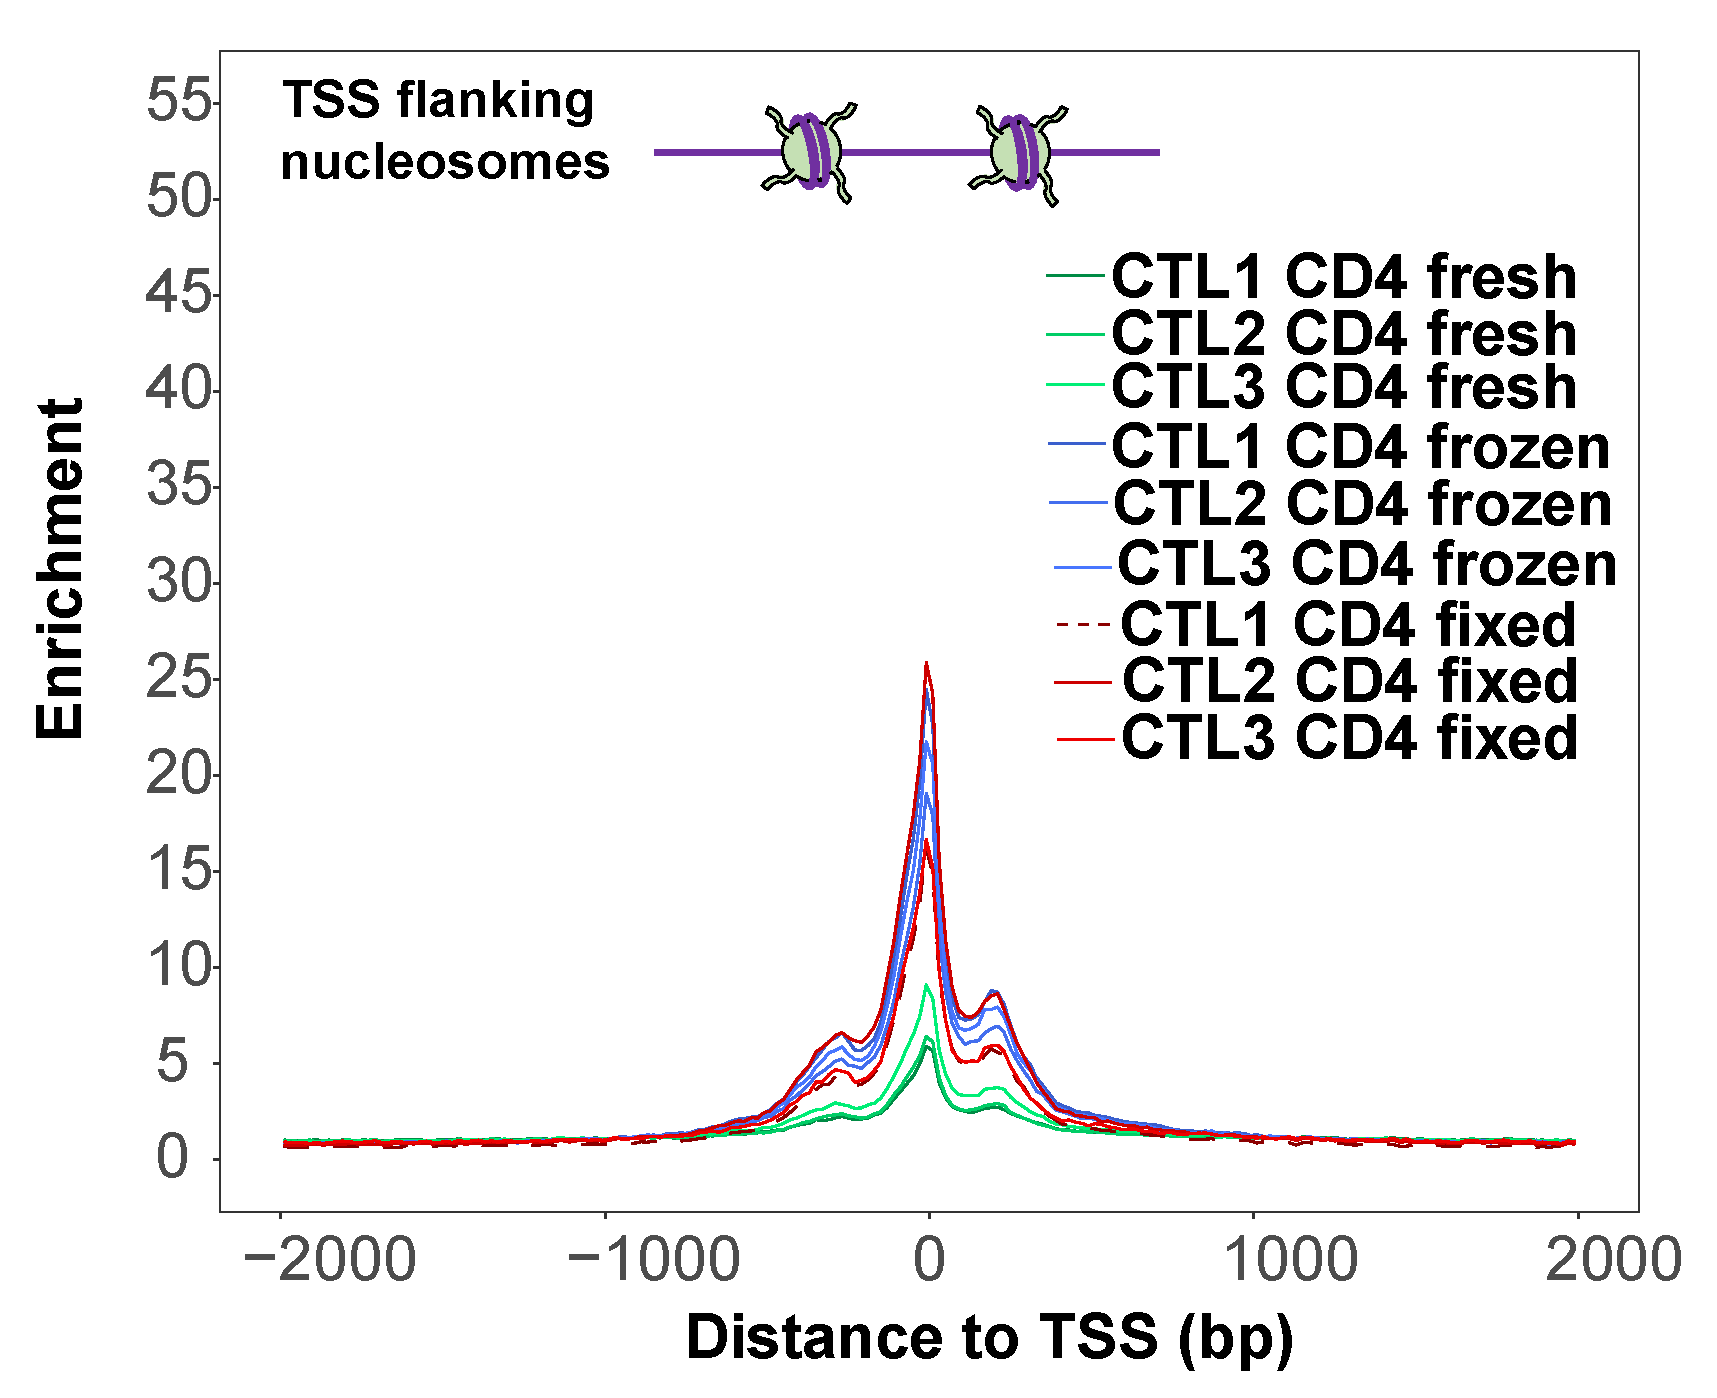
\includegraphics[width=\textwidth]{./Results1/pdfs/Core_ATAC_CD4_fresh_frozen_fixed_dinucleosome_TSS}%
\caption{}
\end{subfigure}
\caption[ATAC-seq enrichment of nucleosome-free and di-nucleosome fragments at the TSS and surroundings in CD14$^+$ monocytes and CD4$^+$ samples for the three conditions.]{\textbf{ATAC-seq enrichment of nucleosome-free and di-nucleosome fragments at the TSS and surroundings in CD14$^+$ monocytes and CD4$^+$ samples for the three conditions.} For each of the samples, nucleosome-free fragments ($<$150bp) or or di-nucleosome (between 260 and 340bp) fragments were selected \textit{in silico}. Enrichment at $+/-$1Kb across all the Ensembl annotated TSS is shown for (A) CD14$^+$ monocytes or (C) CD4$^+$ T cells nucleosome-free fragments and for (B) CD14$^+$ monocytes and (D) CD4$^+$ T cells di-nucleosome fragments. The two nucleosomes flanking the TSS are depicted at the top of each graph.}
\label{figure:Core_ATAC_intra_dinucleosome_tss_enrichment}
\end{figure}



Annotation of the significant peaks identified in each sample (filtered as explained in \ref{peak_filtering}) revealed that the highest proportion of ATAC-seq peaks localised to promoters, introns and intergenic regions (Figure \ref{figure:Core_ATAC_all_conditions_genomic_features}A and B), consistent with previous studies \parencite{Buenrostro2013,Scharer2016}. Interestingly, the ATAC-seq libraries showing higher percentage of peaks at promoter regions corresponded to fixed samples, in which chromatin structure was incompletely preserved, and to fresh CD4$^+$ T cells, with borderline signal-to-noise ratios based on TSS enrichment analysis. The higher percentage of peaks annotated as promoters in in low quality samples revealed reduced ability of these samples to capture genomic features with more moderate chromatin accessibility and bias for the the location of significant robust peaks at the most stable and distinctive open chromatin sites in the genome.

Overall, this analysis demonstrated that the chromatin structure from DSP fixed ATAC-seq libraries was not fully preserved in either of the two cell types, as they all showed a distinct pattern of fragment size distribution in comparison to fresh and frozen samples, as well as loss of nucleosome positioning across the TSS only in CTL1 fixed samples. 

\begin{figure}[htbp]
\centering
\begin{subfigure}{0.5\textwidth}
\centering
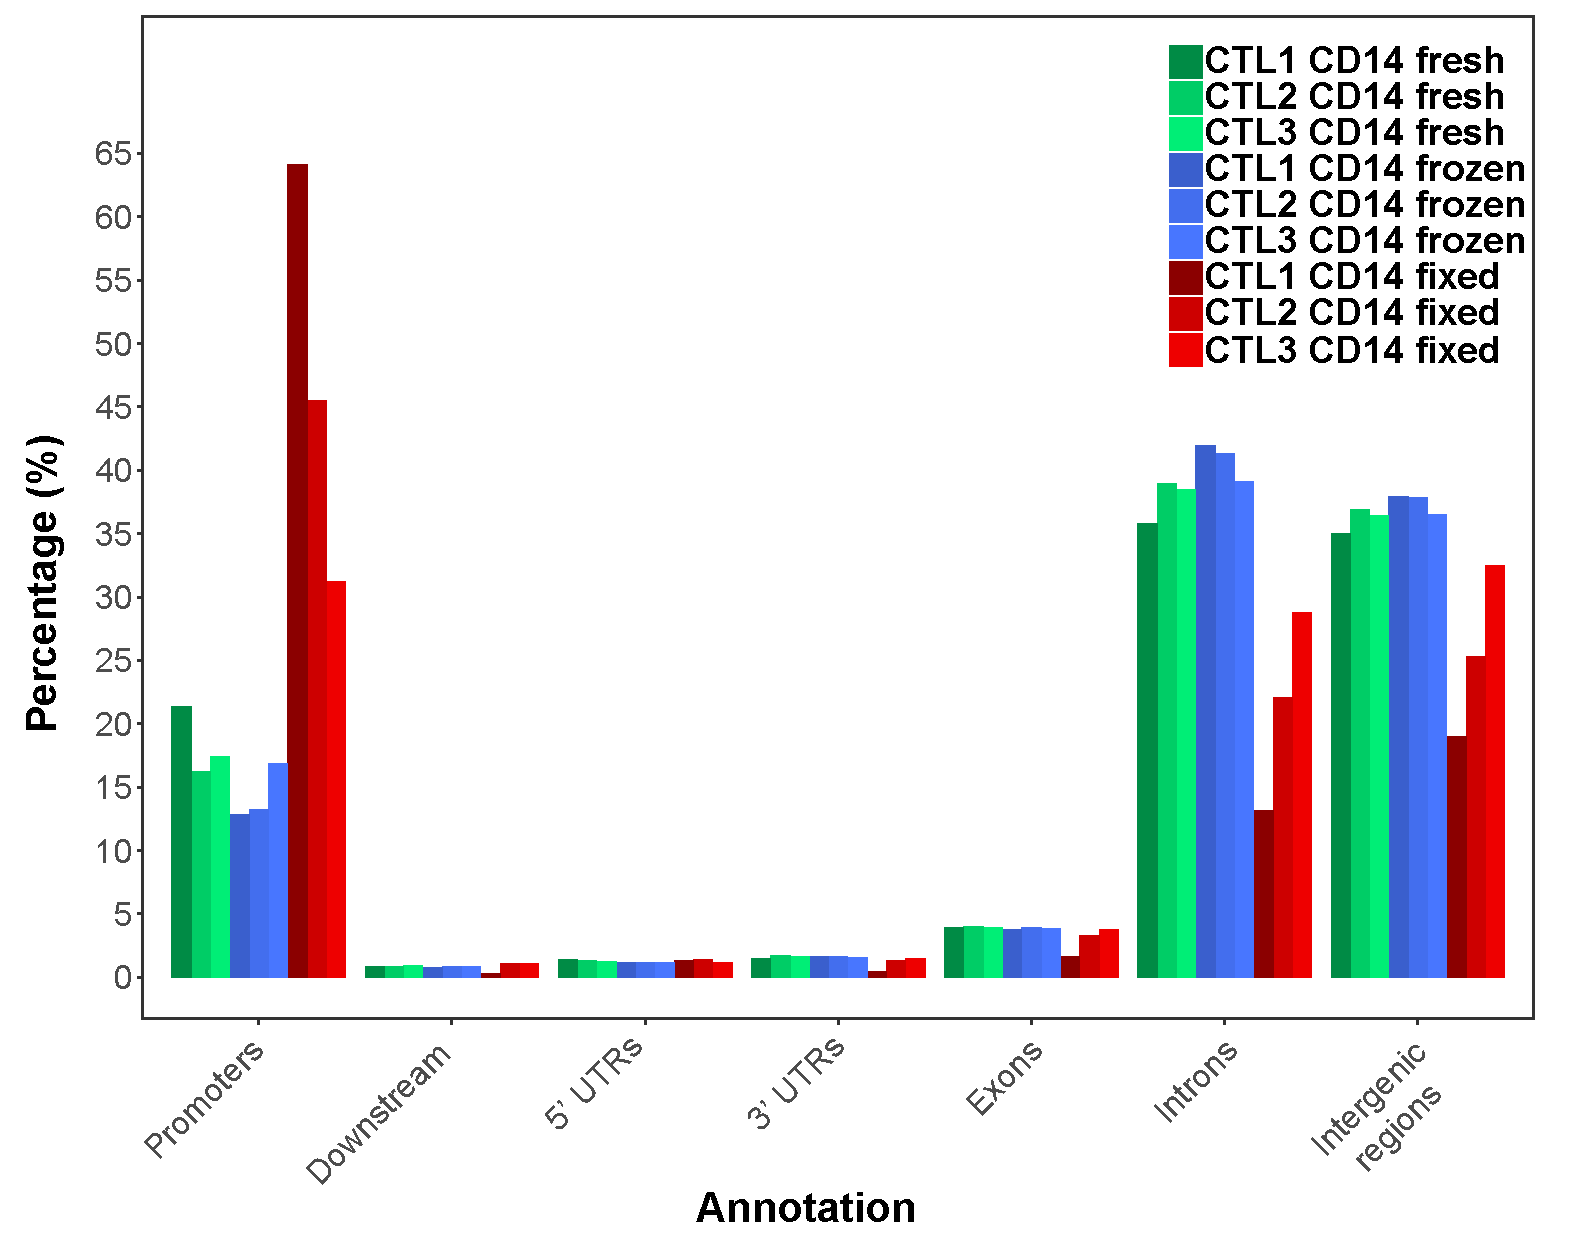
\includegraphics[width=\textwidth]{./Results1/pdfs/Core_ATAC_CD14_fresh_frozen_fixed_IDR_filtered_peak_annotation}
\caption{\textbf{}}
% The percentage sign indicated that the other subfig goes side by side
\end{subfigure}%
\begin{subfigure}{0.5\textwidth}
\centering
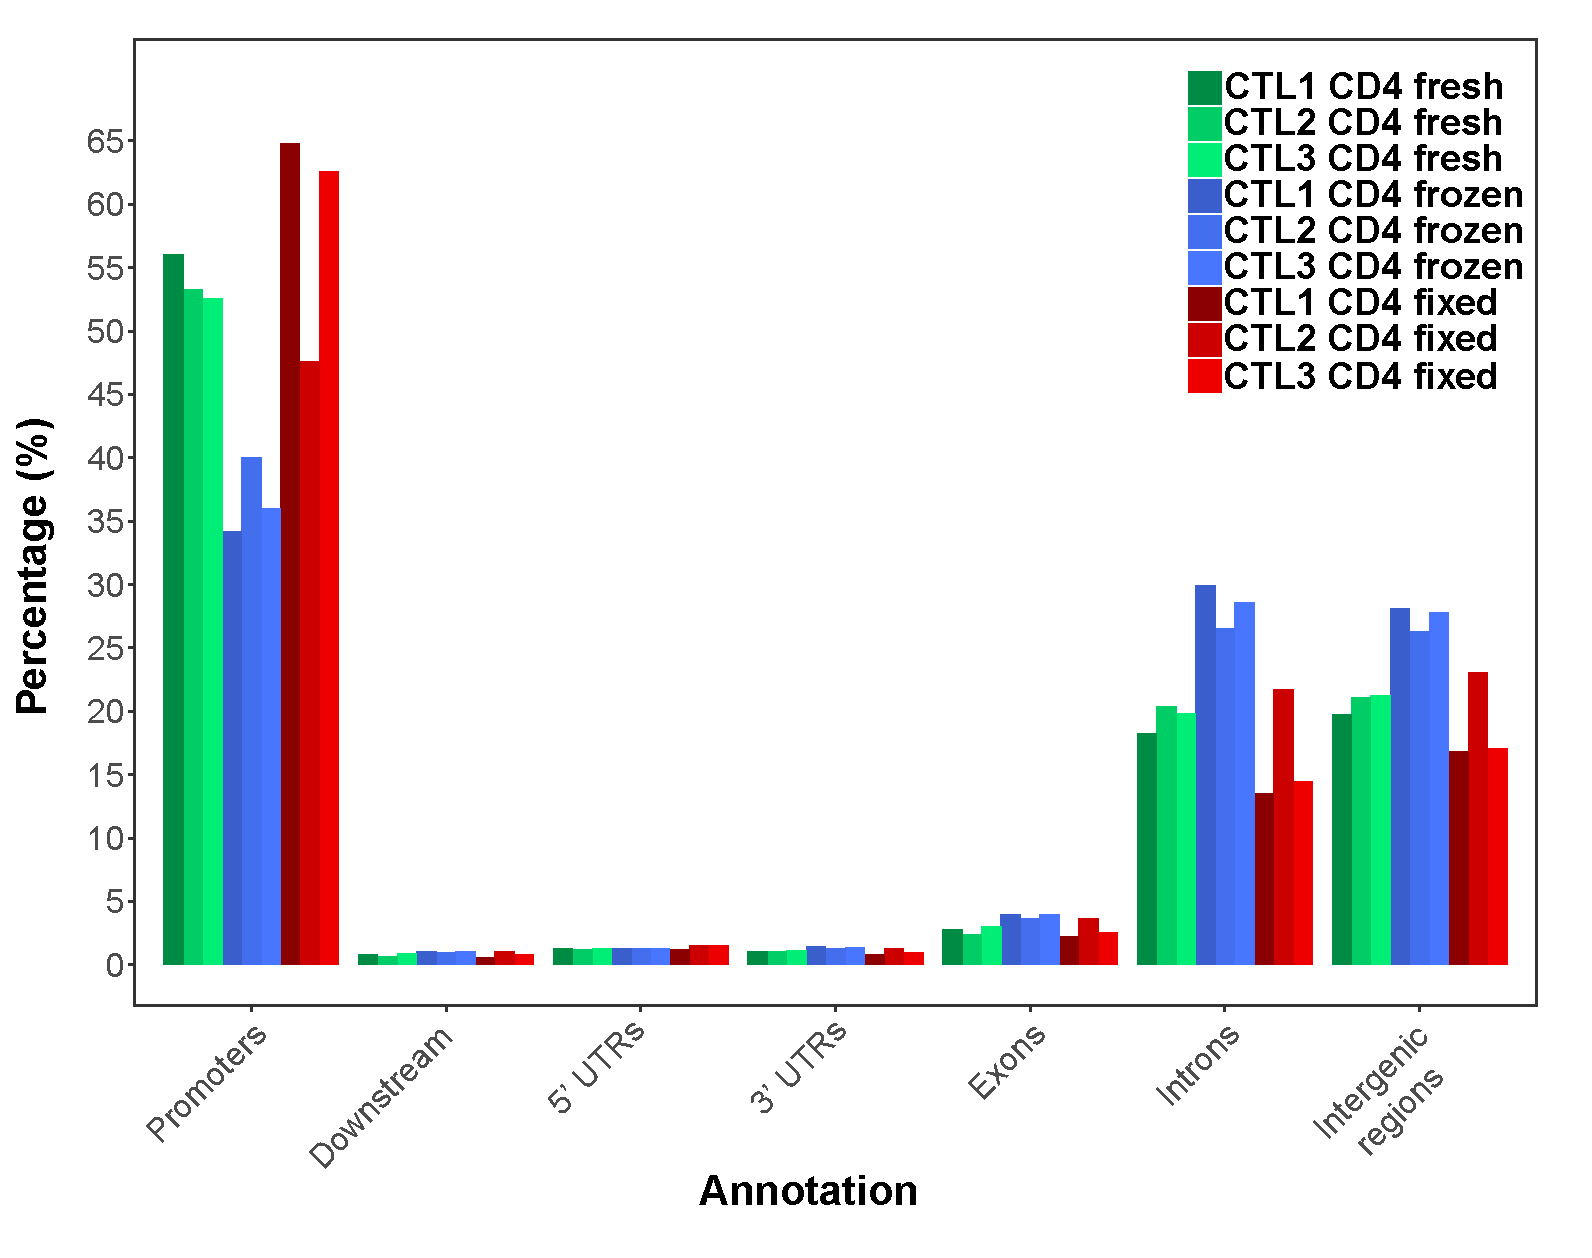
\includegraphics[width=\textwidth]{./Results1/pdfs/Core_ATAC_CD4_fresh_frozen_fixed_IDR_filtered_peak_annotation}
\caption{\textbf{}}
\end{subfigure}
\caption[Genomic features annotation for the ATAC-seq peaks called in each of the fresh,frozen and fixed samples from CD14$^+$ monocytes and total CD4$^+$.]{\textbf{Genomic features annotation for the ATAC-seq peaks called in each of the fresh,frozen and fixed samples from CD14$^+$ monocytes and CD4$^+$.} Overlap was performed between the genomic features and the list of (A) CD14$^+$ monocytes and (B) CD4$^+$ peaks filtered for FDR$<$0.01 in each sample from each of the three conditions (fresh=green, frozen=blue and fixed=red).}
\label{figure:Core_ATAC_all_conditions_genomic_features}
\end{figure} 


Lastly, principal component analysis (PCA) was conducted separately in CD14$^+$ monocytes and CD4$^+$ T cells using the normalised counts retrieved at each of the ATAC peaks from the consensus list built including samples from the three conditions (CP\_CD14\_all\_cond and CP\_CD4\_all\_cond, respectively), with the exception of fixed CTL1 (considerably different from the other two fixed samples). Plotting the first two principal components (PCs) showed sample clustering based on condition in both cell types and demonstrated that the largest source of variability correlated with the way samples were processed (Figure \ref{figure:Core_ATAC_all_conditions_PCA}). 



\begin{figure}[htbp]
\centering
\begin{subfigure}{0.5\textwidth}
\centering
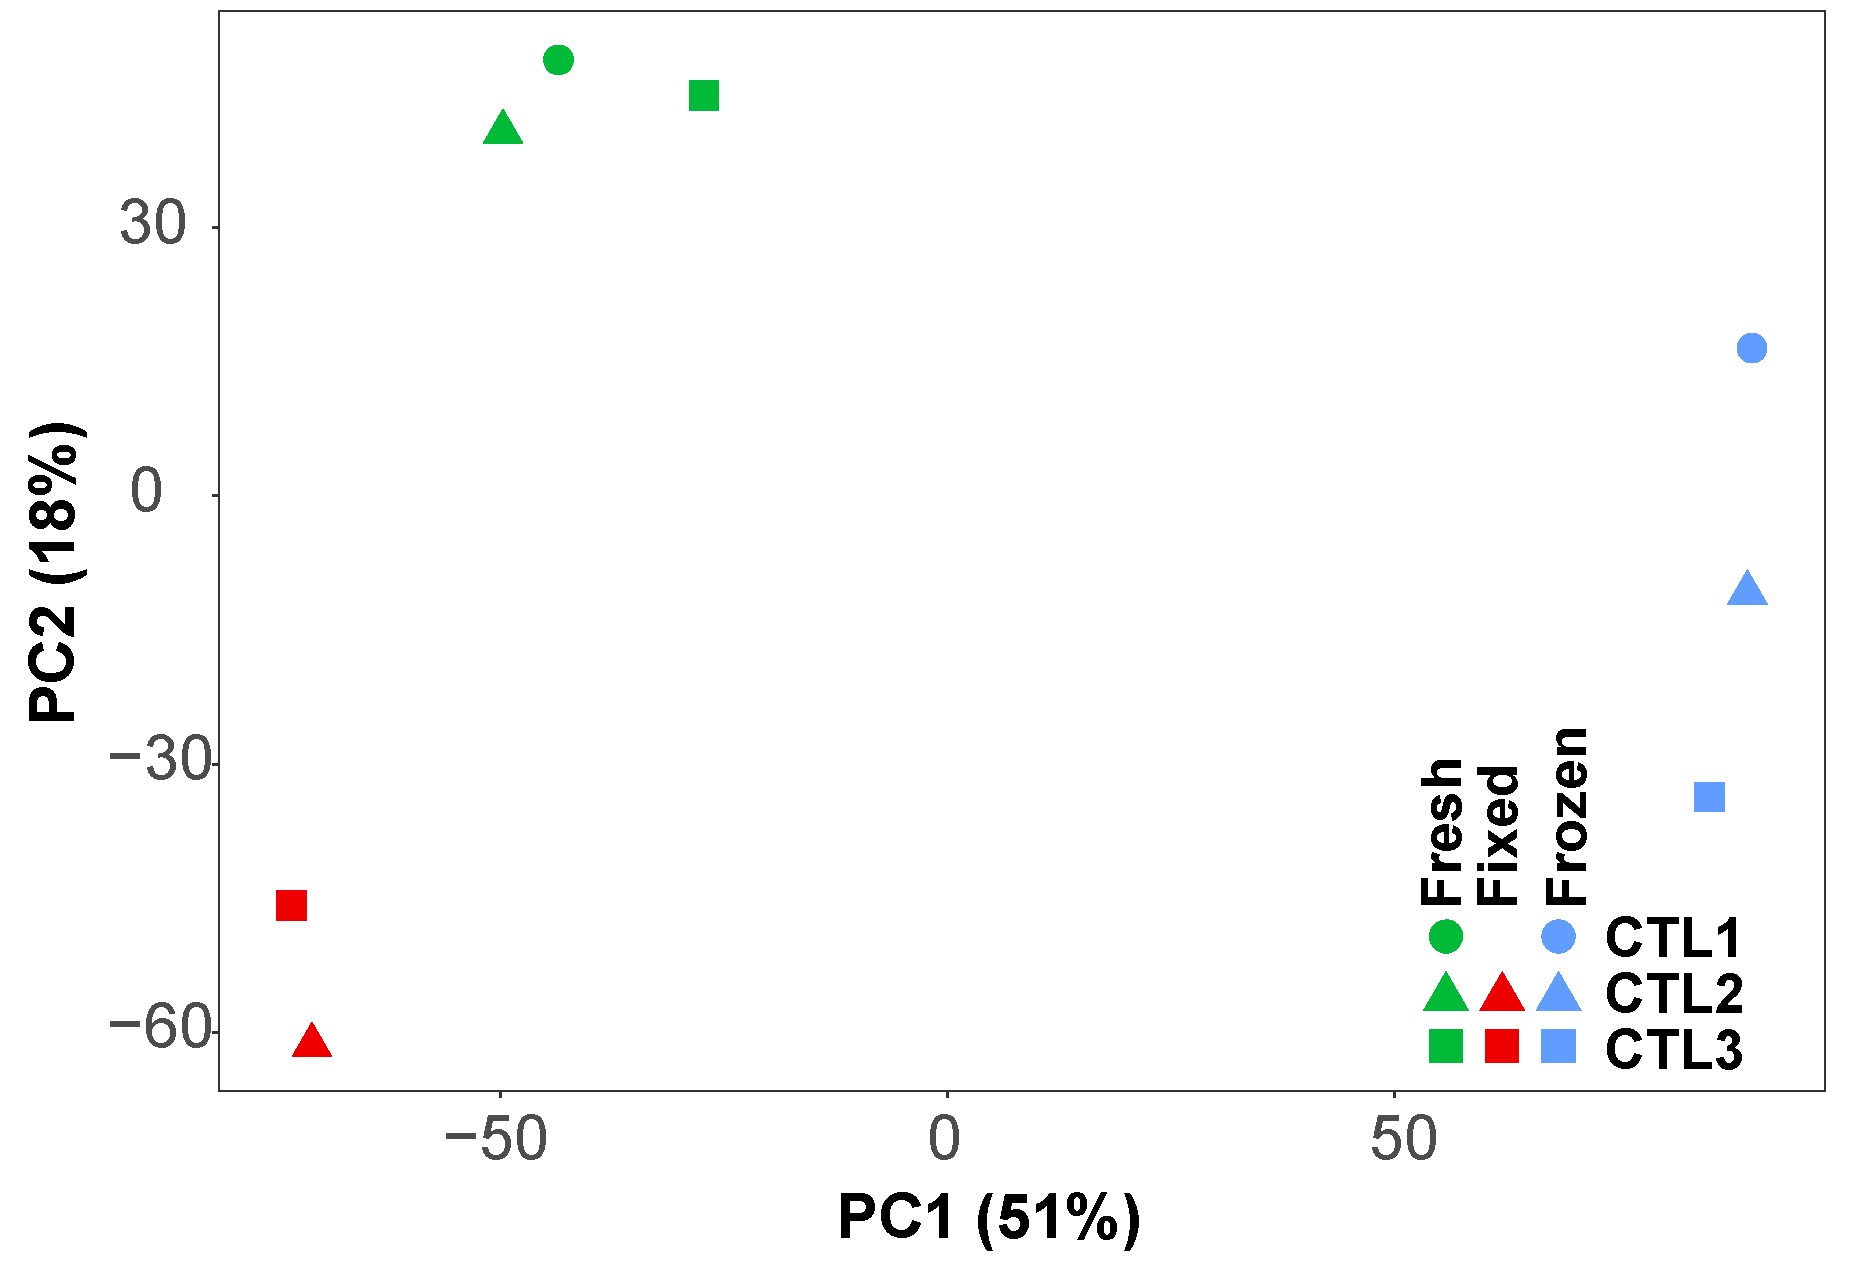
\includegraphics[width=\textwidth]{./Results1/pdfs/Core_ATAC_CD14_fresh_frozen_fixed_no_CTL1_fixed_PCA}
\caption{\textbf{}}
% The percentage sign indicated that the other subfig goes side by side
\end{subfigure}%
\begin{subfigure}{0.5\textwidth}
\centering
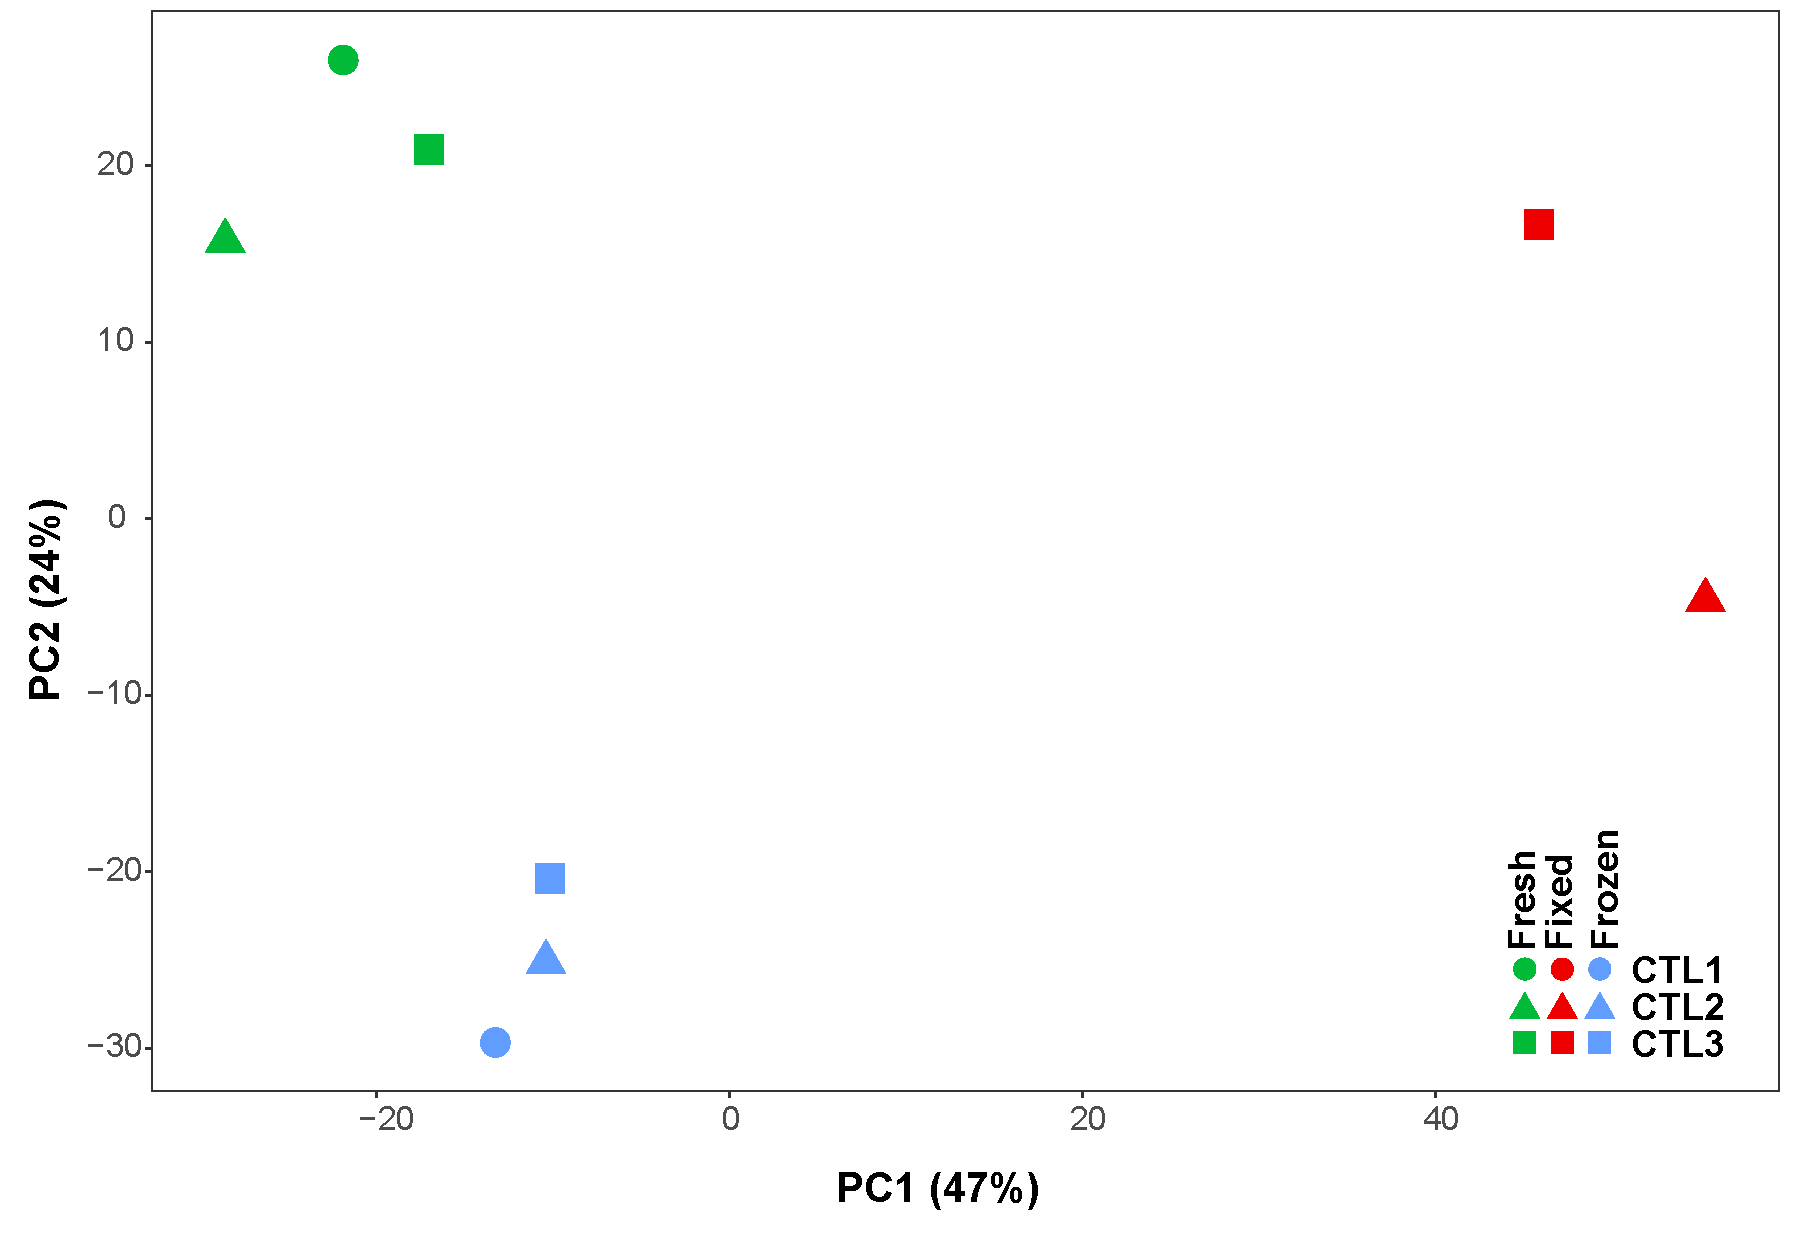
\includegraphics[width=\textwidth]{./Results1/pdfs/Core_ATAC_CD4_fresh_frozen_fixed_no_CTL1_fixed_PCA}
\caption{\textbf{}}
\end{subfigure}
\caption[PCA based on the ATAC-seq chromatin accessibility landscape in fresh, fixed and frozen samples.]{\textbf{PCA based on the ATAC-seq chromatin accessibility landscape in fresh, fixed and frozen samples.} PCA was performed using the normalised counts across the consensus list of ATAC peaks from the combined fresh, fixed and frozen samples (CP\_CD14\_all\_cond and CP\_CD4\_all\_cond) in (A) CD14$^+$ monocytes or (B) CD4$^+$ cells from the same three healthy individuals. The first two PCs (x-axis and y-axis, respectively) of all the regions included in each of the consensus peak list are plotted. Each point represents a sample, where shape codes for individual (CTL1, CTL2, CTL3) and colour means condition (fresh, fixed, frozen). The proportion of variation explained by each principal component is indicated.}
\label{figure:Core_ATAC_all_conditions_PCA}
\end{figure}




\subsubsection{Differential chromatin accessibility analysis between fresh and frozen samples}

In order to determine the effect of the freezing and recovery process in the chromatin landscape of CD14$^+$ monocytes and CD4$^+$ T cells, genome-wide differences between ATAC-seq fresh (biological reference) and frozen were investigated. Since the use of DSP as a fixative was already found to impact preservation of the chromatin structure, differential analysis between fresh and fixed samples was not conducted as the results may be confounded. Comparison between ATAC-seq fresh and ATAC-seq frozen within each cell types was performed using the normalised read counts for the list of ATAC peaks included in the consensus list. Overall, ATAC-seq normalised counts showed high correlation between fresh and frozen samples in the two cell types, with the lowest correlation (R=0.918) found in CD14$^+$ monocytes (Figure \ref{figure:Core_ATAC_all-conditions_correlation}A, B).


\begin{figure}[H]
\centering
\begin{subfigure}[b]{0.45\textwidth}
\centering 
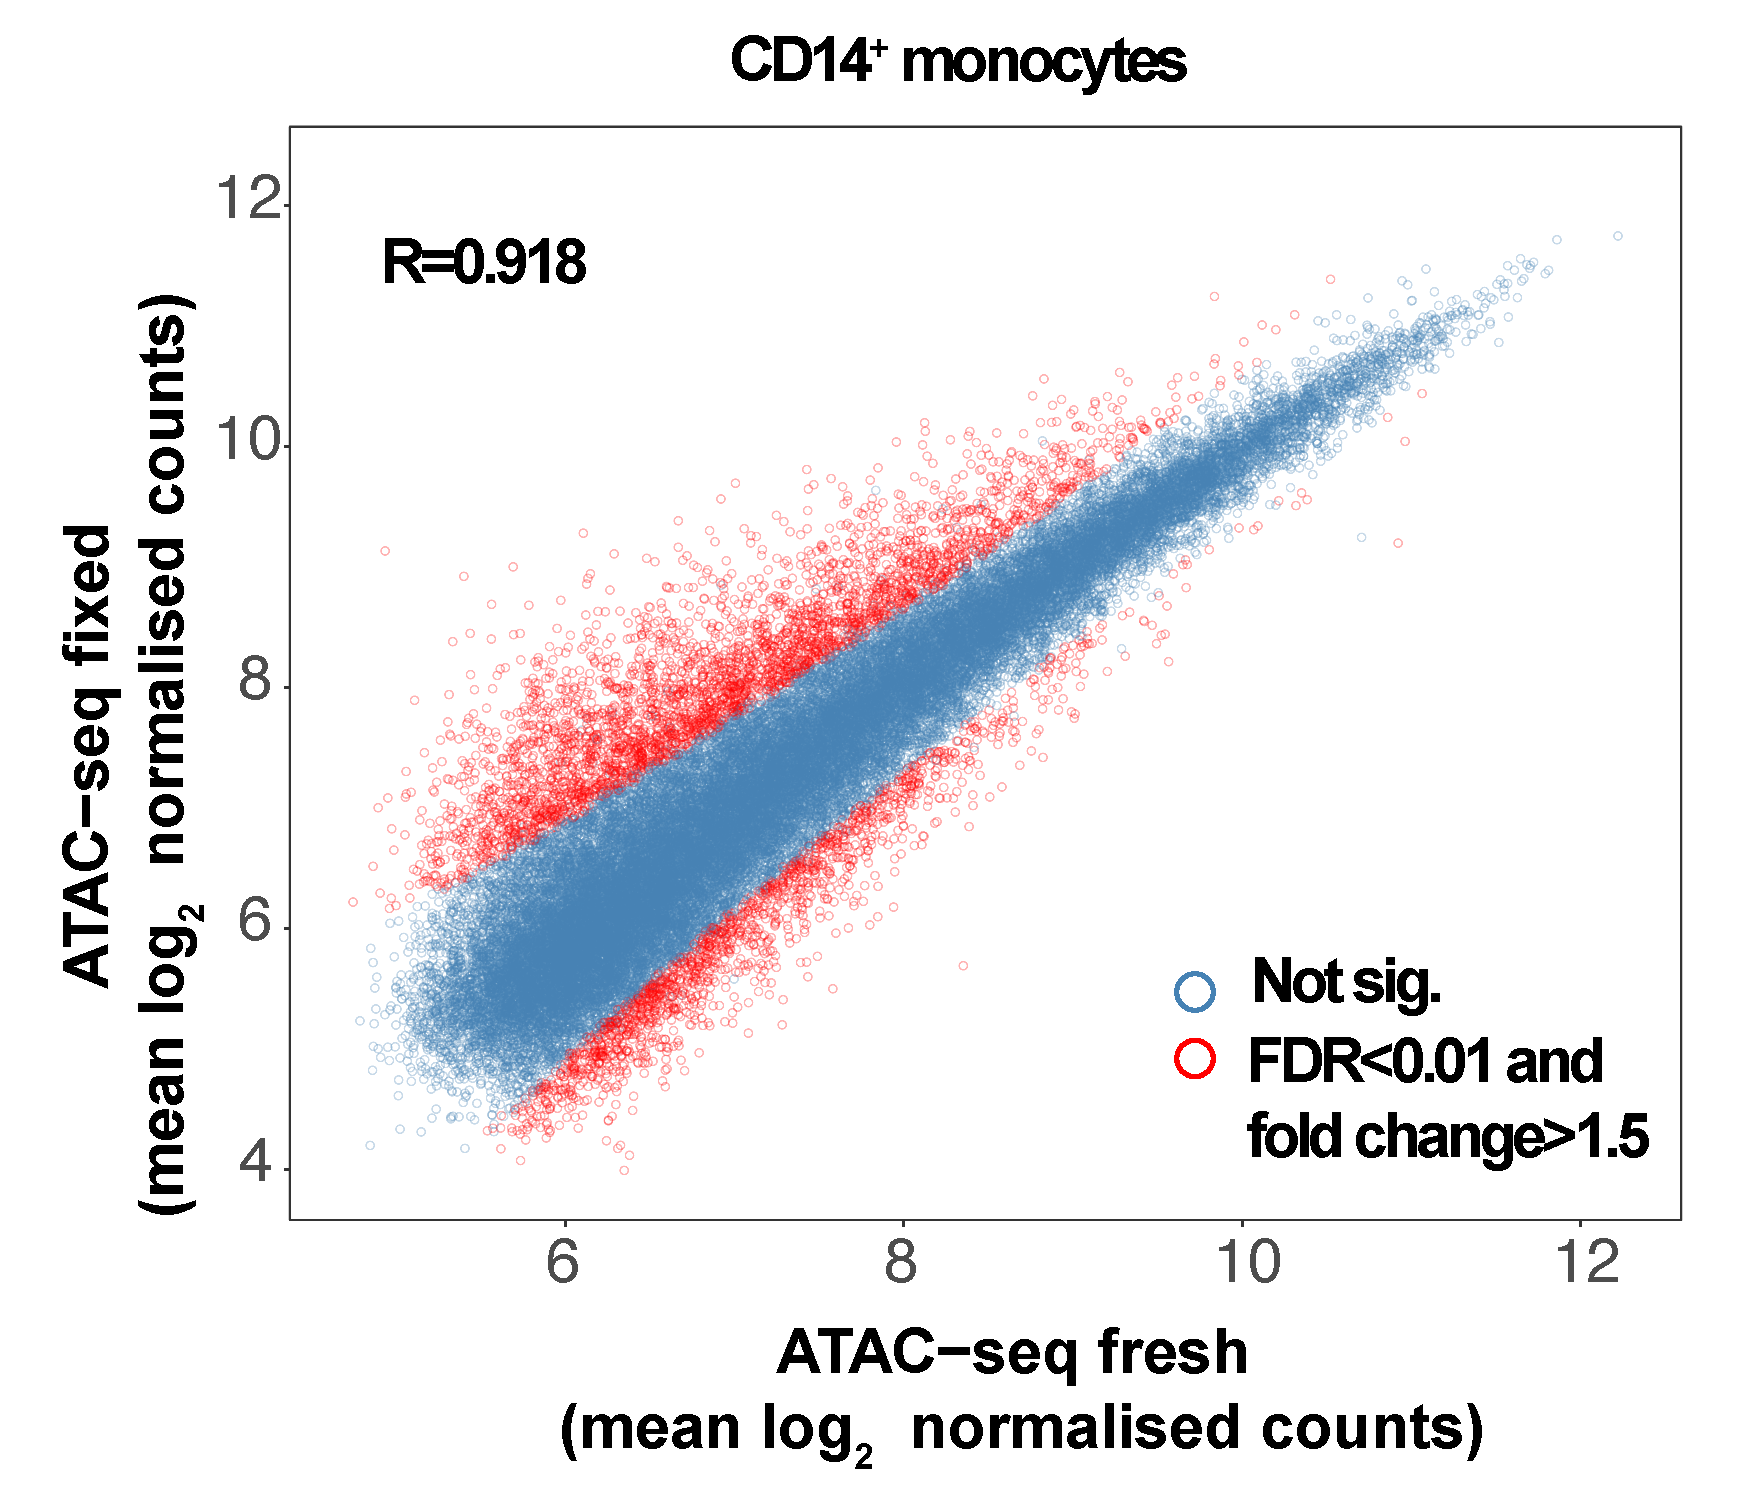
\includegraphics[width=\textwidth]{./Results1/pdfs/Core_ATAC_CD14_fresh_frozen_correlation_counts_small_new}
\caption{}
\end{subfigure}
~
\begin{subfigure}[b]{0.45\textwidth}
\centering 
\includegraphics[width=\textwidth]{./Results1/pdfs/Core_ATAC_CD4_fresh_frozen_correlation_counts_small_new}
\caption{}
\end{subfigure}
\caption[Comparison of the log$_2$ normalised ATAC-seq counts at the consensus list of peaks in fresh and frozen conditions.]{\textbf{Comparison of the log$_2$ normalised ATAC-seq counts at the consensus consensus list of peaks in fresh, fixed and frozen conditions.} Each plot shows the comparison of ATAC-seq log$_2$ mean normalised counts from the CP\_CD14\_all\_cond or CP\_CD4\_all\_cond filtered for background noise (80\% empirical cut-off) between fresh and frozen (A) CD14$^+$ monocytes and (B) CD4$^+$ T cells. Pearson correlation coefficient (R) is indicated.}
\label{figure:Core_ATAC_all-conditions_correlation}
\end{figure}
	


The differential chromatin accessibility analysis between ATAC-seq fresh and frozen samples using DEseq2 revealed a total of 5,123 and 177 significant DARs (FDR$<$0.01 and fold change$>$1.5) and a larger proportion of regions (12.6 and 1.3\%)changing chromatin accessibility between fresh and frozen samples in CD14$^+$ monocytes compared to CD4$^+$ T cells, respectively. Nevertheless, the percentage of sites identified as DARs in relation to the total number of investigated regions for both cell types suggested only moderate changes in the chromatin accessibility landscape between fresh and frozen conditions. 


%To further assess the differences in chromatin accessibility, differential chromatin accessibility analysis between ATAC-seq fresh and ATAC-seq fixed or frozen at each of the ML\_CD14\_all\_cond and ML\_CD14\_all\_cond peaks was performed using DESeq2. The number of significant DARs (FDR$<$0.01) reported for in each of the comparisons mirrored the PCA analysis results (Table \ref{tab:Core_ATAC_all_conditions_DARs}). In CD14$^+$ monocytes, the largest number of DARs (5,269) was reported when comparing ATAC-seq frozen to the fresh reference state. Conversely, in CD4$^+$ the greatest differences in chromatin accessibility were found between fresh and fixed ATAC-seq samples (1,564 DARs).  	
	
	
\begin{table}[htbp]
%\setlength{\tabcolsep}{20pt} only to stretch the columns if you want
%\renewcommand{\arraystretch}{1.5}
\centering
\begin{tabular}{@{} c c c}
\toprule
\textbf{Cell type} & \textbf{Total regions in} & \textbf{DARs} \\
                   & \textbf{consensus list}   & \textbf{(percentage)} \\
\midrule
\midrule
CD14$^+$ monocytes & 40,600                    & 5,123 (12.6\%) \\
CD4$^+$            & 13,025                    & 177  (1.3\%) \\
\bottomrule
\end{tabular}
\medskip %gap
\caption[Summary results from the differential chromatin accessibility analysis comparing ATAC-seq frozen or fixed chromatin landscape to the reference ATAC-seq fresh.]{\textbf{Summary results from the differential chromatin accessibility analysis comparing ATAC-seq frozen or fixed chromatin landscape to the reference ATAC-seq fresh.} The number of regions in the consensus list (CP\_CD14\_all\_cond or CP\_CD4\_all\_cond) following filtering for background counts using 80\% cut-off and the number of significant DARs (FDR$<$0.01 and fold change$>$1.5) are shown. In brackets the percentage of DARs over the total number of regions included in the differential analysis is indicated.}
\label{tab:Core_ATAC_all_conditions_DARs}
\end{table}
\bigskip %bigger space


In order to identify biological processes that may altered by the changes in chromatin accessibility between conditions, enrichment analysis was conducted using as input the genes proximal ($<$5Kb) to the significant DARs (FDR$<$0.01 and fold change$>$1.5) identified in each cell type. Significantly enriched Gene Ontology (GO) biological processes (FDR$<$0.01) were only identified for CD14$^+$ monocytes (Figure \ref{figure:Core_CD14_fresh_vs_frozen_GOBP_barplot}). This included changes in chromatin accessibility of regions in proximity to genes involved in cell shape and cell adhesion, lipopolysaccharide-mediated signalling, inflammation and signal transduction, amongst others, suggesting that CD14$^+$ monocytes may undergo some activation as a result of the cryopreservation and subsequent recovery in incubation. 



\begin{figure}[htbp]
\centering
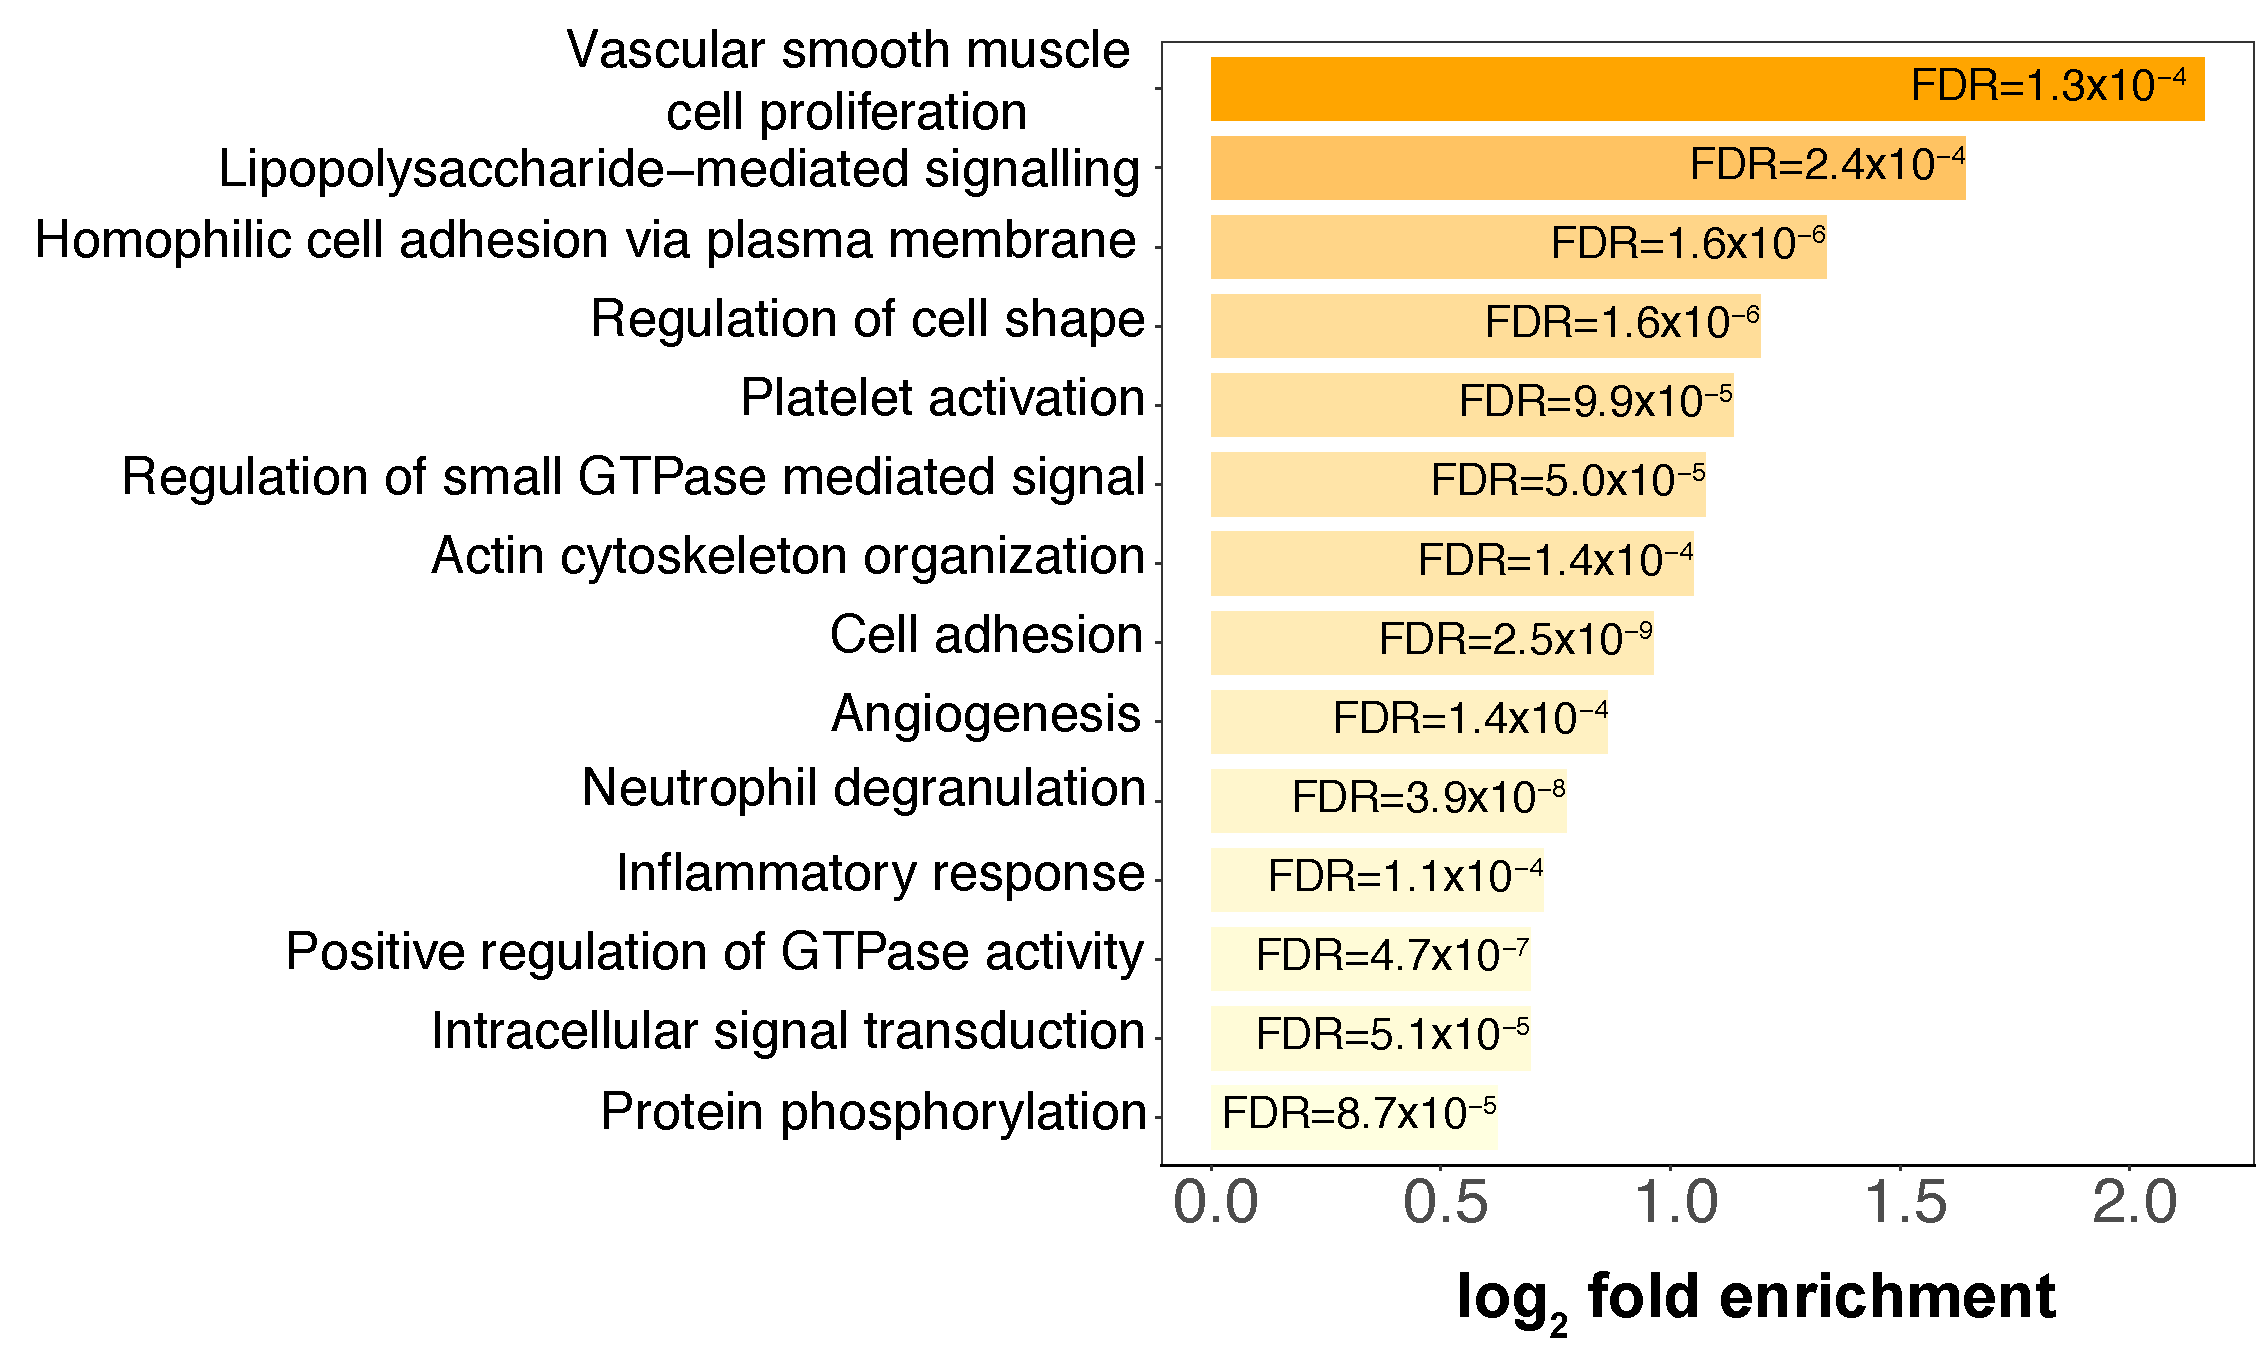
\includegraphics[width=0.7\textwidth]{./Results1/pdfs/ATAC_core_CD14_fresh_vs_frozen_GOBP_barplot}
\caption[Top fourteen Gene Ontology biological processes enriched for DARs between ATAC-seq fresh and ATAC-seq frozen samples in CD14$^+$ monocytes.]{\textbf{Top fourteen gene Ontology biological processes enriched for DARs between ATAC-seq fresh and ATAC-seq frozen samples in CD14$^+$ monocytes.} The barplot shows the top fourteen most significant (FDR$<$0.01) Gene Ontology (GO) biological processes enriched for genes proximal to DARs identified between fresh and frozen CD14$^+$ monocytes.  The GO terms are ordered based log$_2$ fold change enrichment and the exact significance (FDR) for each of them is also indicated.}
\label{figure:Core_CD14_fresh_vs_frozen_GOBP_barplot}
\end{figure}


	
For example, three of the DARs identified when comparing ATAC-seq fresh to ATAC-seq frozen CD14$^+$ were found at the promoter, an exon and the 3'UTR of the \textit{TNFSF14} gene and showed greater accessibility in frozen compared to fresh samples (Figure \ref{figure:Core_CD14_differential_TNFSF14}. TNFSF14 is the ligand for a receptor from the TNF-receptor superfamily and is involved in T cell activation, induction of apoptosis and  also in bone destruction mediated by monocytes and synovial cells interactions in RA. 

	
	
	
\begin{figure}[htbp]
\centering
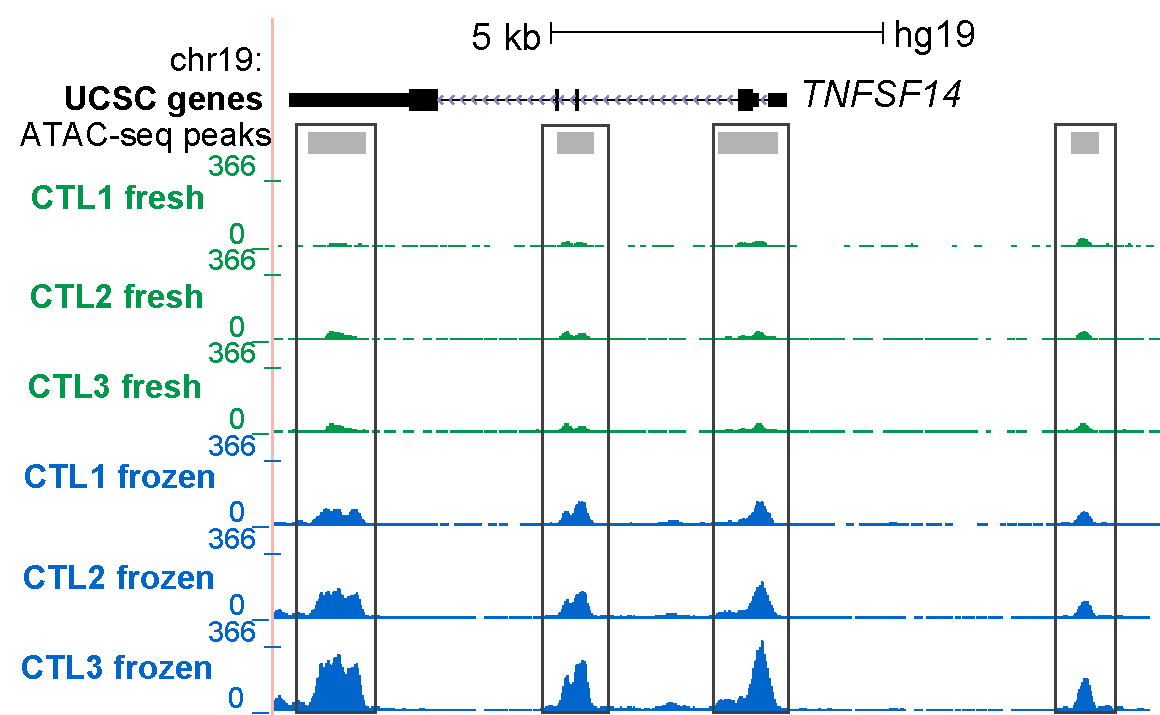
\includegraphics[width=0.65\textwidth]{./Results1/pdfs/Core_CD14_TNFSF14_track_UCSC}
\caption[Differential chromatin accessibility at the \textit{TNFSF14} gene between ATAC-seq fresh and ATAC-seq frozen in CD14$^+$ monocytes.]{\textbf{Differential chromatin accessibility at the \textit{TNFSF14} gene between ATAC-seq fresh and ATAC-seq frozen in CD14$^+$ monocytes.} UCSC Genome Browser view illustrating the normalised read density (y-axis) at four significant (FDR$<$0.01 and fold change$>$1.5) DARs (x-axis) within and upstream the \textit{TNFSF14} gene in CD14$^+$ monocytes. The four DARs were more accessible in ATAC-seq frozen when compared to ATAC-seq fresh. Tracks are colour-coded by condition(green=fresh and blue=frozen).}
\label{figure:Core_CD14_differential_TNFSF14}
\end{figure} 	






\section{Discussion}

The aim of this chapter was to establish a data analysis pipeline for ATAC and compare various experimental protocols, as this was the first time this technique was used in the research group. A particular focus was to consider appropriate methodologies for clinical studies, where sample availability and quality may be severely limiting. A number of alternative protocols, metrics and algorithms described in early ATAC reports were evaluated in the pilot experiments presented in this chapter. This enabled the establishment of a pipeline and approach to be implemented for investigation of the psoriasis and PsA chromatin landscape (Chapters \ref{ch:Results2} and \ref{ch:Results3}).

\subsection{ATAC: methodological aspects and pipeline establishment}

At the time of the first ATAC-seq publication \parencite{Buenrostro2013}, well established protocols for complete processing and data analysis of ATAC were lacking. Since then, several publications have implemented ATAC-seq and modifications of this protocol together with a wide range of data analysis strategies to answer different biological questions (Table \ref{tab:ATAC_comparative_methods}) as well as alternative protocols such as THS-seq to assess chromatin accessibility in low number of cells.

The data and analysis presented in this chapter has confirmed some limitations of the ATAC-seq and Fast-ATAC protocols. Quality assessment and variability across samples was difficult to detect through pre-sequencing library quality control based on relative abundance of the different DNA fragment sizes. Successful profiles of DNA relative abundance for the ATAC libraries, showing nucleosome patterns would still lead to libraries with high background noise when visualising read density in the UCSC Genome Browser. This required the identification and establishment of appropriate data analysis and quality control measures beyond pre-sequencing library quality assessment.

In this chapter different quality metrics were explored, including TSS enrichment and FRiP. Both correlated well with the overall differences in sample quality from the ATAC-seq libraries used as an exemplar here. Importantly, TSS and FRiP were shown to be independent of sequencing depth, and therefore can be applied in low depth sequenced samples when performing optimisation or preliminary quality control before increasing the coverage, as also recently shown in other studies \parencite{Corces2017}. Similarly to TSS, FRiP proved to be informative in evaluating signal-to-noise ratios; however it relies on peak calling and thus is more likely to be biased by the filtering strategy. In agreement with these findings, enrichment of ATAC signal across Ensembl annotated TSS is now recommended by ENCODE as the preferred means of assessing overall sample quality, and was implemented as the metric to evaluate signal-to-noise in our pipeline. 

The variability in quality of ATAC-seq libraries was also addressed at the peak calling level in this chapter, with the implementation of a peak filtering strategy that for each sample could identify good quality and reproducible peaks using IDR analysis between pseudoreplicates. This approach was demonstrated to reduce  repetitive and non meaningful regions that could be confounders for downstream analysis. In terms of sequencing depth, analysis in this chapter showed that approximately 15 to 20 million reads after filtering were the minimum required to identify an appropriate proportion of accessible regions (peaks) as well as to obtain meaningful results in the peak filtering based on pseudoreplicate IDR analysis. These observations have also been confirmed by Qu and colleagues \parencite{Qu2017}, where IDR analysis at different sequencing depths was used to evaluate consistency across replicates but not implemented for peak filtering.

Establishment of appropriate measurements for post-sequencing library quality control allowed formal testing, beyond the conditions from Buenrostro's publication, for the effect of transposition times, which one of the variants that can affect the quality of ATAC libraries in a cell type specific manner. At the start of the project transposition for 40 min appeared the most appropriate for all cell types according to pre-sequencing library quality control (relative abundance of DNA library fragment sizes). Longer transposition times are known to reduce the length of the yielded fragments and to increases, to some extent, the abundance of NFF \parencite{Raurell-Vila2018}. Assessment of three different transposition times for the ATAC-seq protocol showed minor and heterogenous effects on the NFF/mNBF ratio and the signal enrichment across the TSS for the different cell types. For example longer transposition showed a slight increase of NFF abundance in CD14$^+$ monocytes but reduction in CD8$^+$ cell. Altogether, these results from a single replicate for each transposition time suggested that changes in the duration of the tagmentation reaction at this scale do not have considerable impact on the ATAC-seq fragment size distribution and the signal-to-noise ratios, with the largest variability being cell type dependent.

The use of the improved Fast-ATAC protocol addressed some of the limitations identified by the ATAC-seq data generated within our group. Using only one replicate, Fast-ATAC showed reduction in the percentage of mitochondrial reads in all cell types when compared to ATAC-seq. Retrospective analysis comparing ATAC-seq to Fast-ATAC-seq using all samples described in this thesis confirmed that Fast-ATAC significantly reduced the percentage of mitochondrial reads in the four studied cell types (unpaired Wilcoxon signed-ranked test p-values$<$4.1x10$^{-05}$) (Figure \ref{figure:Comparison_ATACseq_vs_fastATAC_all_thesis_samples}A). Regarding signal intensity of the libraries, a trend for improved signal-to-noise when using Fast-ATAC was only found in CD14$^+$ monocytes and CD$^+$ cells in the preliminary analysis using one replicate per cell type. Conversely, the retrospective analysis including all the libraries generated in this thesis only showed statistically significant increased TSS fole-enrichment in CD4$^+$ cells (unpaired Wilcoxon signed-ranked test p-values=0.024) and was not a significant improvement for any of the remaining three haematopoietic cell types (Figure  \ref{figure:Comparison_ATACseq_vs_fastATAC_all_thesis_samples}B). In fact, Corces and colleagues Fast-ATAC publication only showed data demonstrating improved TSS by Fast-ATAC for CD4$^+$ T cells \parencite{Corces2016}. In contrast, the Omni-ATAC protocol publication included a comprehensive comparison of the three ATAC protocols across a large number of cell types showing that Fast-ATAC did not improve TSS fold-enrichment when compared to ATAC-seq in a number of the haematopoietic cells, for example CD19$^+$ cells, in line with the results presented in this chapter \parencite{Corces2017}.

%pre-sequencing library quality control based on relative abundance of the different DNA fragment sizes. Successful profiles of DNA relative abundance for the ATAC libraries,


\subsection{The challenges of performing differential chromatin accessibility analysis}
%Until ATAC-seq release, limited research had been performed to investigate differences in chromatin accessibility, and mainly used data from cell lines \parencite{Degner2012}. 
Studying chromatin accessibility in clinical samples first requires the definition of a consensus list of accessible regions for which no accepted method has been agreed. In this work, a consensus list of ATAC peaks containing all the peaks identified in at least 30\% of the samples included in analysis has been chosen. This represents an unbiased approach to include peaks that can vary across individuals (regardless of biological subgroup) but still be differentially accessible across conditions. Other publications have preferred building condition-specific consensus lists of peaks or simply including all the significant peaks called in all the analysed samples \parencite{Alasoo2018, Thurner2018}. 

When used for differential analysis, an additional filtering step has been implemented to account for background noise in peaks included in the consensus list for being significant (present) in at least 30\% of all the samples but did pass quality filtering (therefore considered absent) in a number of them. In terms of the algorithm to perform normalisation and differential chromatin accessibility analysis, no consensus has been reached in the literature. The majority of the studies reviewed at the time of implementing differential analysis were peak-based and relied on RNA-seq or microarray algorithms such as EdgeR, limma or DESEq2 (Table \ref{tab:ATAC_comparative_methods}). The analysis here, revealed DESeq2 as a more stringent method compared to quantile normalisation \& limma voom. Limma has been reported to be affected by low quality samples and that may also explain the increase in differential hits observed when compared to DESEq2 \parencite{Alasoo2018}. For both methods, the implementation of the additional filtering cut-off to control for high number of background reads has shown a reduction in the number of significant differentially accessible regions. Given the difficulties of recruiting large numbers of suitable clinical samples, DEseq2 in combination with the additional filtering step was chosen at the time of the study as an appropriately stringent method to account for variability in sample quality and to control, to some extent, for potential false positive hits. As specific tools for ATAC analysis are developed, further comparison of the different outputs will be of interest in future work.


\subsection{Studying the chromatin landscape from psoriasis skin biopsies}
At the time of writing, only RNA-seq studies have been performed in keratinocytes from psoriasis skin biopsies. The relevance of keratinocytes in psoriasis pathophysiology and the ability to sample this tissue represented a great opportunity to investigate the chromatin accessibility landscape at the main site of inflammation using ATAC. The low signal-to-noise ratios observed in ATAC-seq libraries generated from lesional keratinocytes in suspension was hypothesised to be the result of low cell viability together with under-transposition of the nuclei due to insufficient Tn5 and/or poor cell lysis. The poor performance of ATAC-seq (both, Buenrostro \textit{et al.} 2013 and Bao \textit{et al.} 2015 versions) and Fast-ATAC protocols on NHEKs and keratinocytes isolated from skin biopsies on the culture plate, without prior cell dettachment using trypsinisation, suggested that the main limitation was intrinsic to the cell type and not driven by compromised cell viability. Importantly, ATAC-seq on tcultured NHEKs using Bao \textit{et al.} protocol (ATAC 2) not only failed to reproduce the successful results presented in the publication but also did not show improvement in the quality of the library by increasing the Tn5 concentration, reinforcing the lysis step as the main limitation.

The characteristic insoluble protein structure synthesised by keratinocytes that, as differentiation progresses, replaces the plasma membrane is likely to difficult cell permeabilisation and efficient transposition. In fact, inefficient lysis by the Buenrostro \textit{et al.} 2013 ATAC-seq version of the protocol has been demonstrated to cause poor quality libraries in breast tissue biopsies \parencite{Fijiwara2019}. The Omni-ATAC protocol lysis buffer combines three non-ionic detergents (NP-40, digitonin and Tween-20) at a greater detergent concentration (0.21\% vs 0.1 and 0.01\% in ATAC-seq and Fast-ATAC, respectively) resulting in a more efficient cell lysis \parencite{Corces2017}.  The Omni-ATAC protocol demonstrated a considerable improvement in performance compared to ATAC-seq and Fast-ATAC in NHEKs, consistent with data presented by Corces \textit{et al.} 2017 in the same cell type. The two-fold increase in detergent concentration used by the Omni-ATAC protocol compared to ATAC-seq (from 0.1 to 0.021\%) is consistent with the failure of the 0.025\% digitonin concentration tested with the Fast-ATAC protocol C4 to improve cell lysis. Furthermore, the Omni-ATAC publication also showed quality measures for ATAC-seq and Fast-ATAC data in NHEKs, further supporting the poor quality of my results when using those protocols. 

Altogether, the successful results of Omni-ATAC in NHEKs encourage testing its performance in keratinocytes isolated from skin biopsies and open an avenue to ultimately explore the chromatin landscape in lesional and uninvolved skin from psoriasis patients. Unfortunately, this aim was not compatible with the time frame of this thesis and could be conducted as future work for the project.



\subsection{Characterisation of the effect of preservative techniques in the chromatin landscape}
The use of clinical samples sometimes involves logistical limitations that require sample preservation. At the time of starting this thesis the Oxford Genomics Centre at the WHG had implemented the use of DSP as a compatible fixative for microfluidics-based scRNA-seq methods \parencite{Attar2018}. Moreover, at the time of the experiment ATAC-seq was incompatible with traditional fixatives such as formaldehyde. It was therefore of interest to test the ability of this fixative to maintain the chromatin structure prior to performance of ATAC-seq, which would allow simulatanous preservation of gene expression and chromatin accessibility in the samples. Despite of DSP showing appropriate preservation of cell and RNA integrity with minimal differences in scRNA-seq when compared to fresh material \parencite{Attar2018}, my data demonstrated altered chromatin structure in the the fixed ATAC-seq libraries which showed altered fragment size distribution profiles with partial or total loss of NFF when compared to the fresh and frozen libraries. The performance of DSP was particularly poor in CTL1 samples, which despite showing relatively high abundance of di-nucleosome fragments failed to reproduce the position of the TSS flanking nucleosomes, suggesting nucleosome displacement. Although the cross-link of free amine groups upon DSP fixation allows to preserve tissue and RNA integrity \parencite{Espina2013Attar2018}, the data here presented suggests that this is not sufficient to maintain the chromatin structure of cells likely due to lack of cross-linking between DNA and proteins. 

Cryopreservation of PBMCs had historically been used but formal assessment of the effect of this process on the chromatin landscape of different cell types had not yet been conducted. In this chapter cells were recovered in cell culture after thawing and subsequently sorted using FACS, as it has been done historically in the group prior to downstream analysis. As expected, the chromatin structure of the frozen ATAC-seq samples was appropriate and similar to the fresh libraries. PCA demonstrated that global differences in chromatin accessibility due to condition were greater than the differences between individuals, as fresh and frozen samples could be clearly separated in both cell types. Differential chromatin accessibility analysis revealed a moderate number of DARs between frozen and fresh samples in both cell types, with a greater percentage in CD14$^+$ monocytes compared to CD4$^+$ T cells. This suggested that CD14$^+$ monocytes were more sensitive to the cryopreservation and recovery process than T cells, which was further supported by the enrichment of CD14$^+$ monocytes DARs in biological processes characteristic of cell activation, including cell adhesion and shape, LPS response and inflammation. Cryopreservation of PBMCs using DMSO has been demonstrated to alter transcription of a number of genes involved in stress responses, immune activation and cell death \parencite{Yang2016}, in line with the results presented here. Importantly, cryopreservation of monocytes and immature DCs have shown a skewed profile compared to fresh counterparts \parencite{Meijerink2011}.  The impact of cryopreservation and thawing on the chromatin landscape may have been minimised by avoiding the recovery step in culture and proceeding directly into PBMC staining with FACS antibodies; however additional data would be required to confirm this hypothesis.

It is important to note that the results presented here could be limited by the small sample size and borderline quality of some of the libraries, particularly CD4$^+$ fresh samples, likely due to the intrinsic inconsistency issues of the ATAC-seq protocol. This may have impacted to some extent the power to identify DARs between fresh and frozen CD4$^+$ ATAC-seq samples. Nevertheless, this data still provides some useful information regarding the effect of using DSP in sorted cell populations and cryopreservation of PBMCs, which should be considered when planning the experimental design. Following these results, fresh isolated cells were used in the experiments presented in Chapters \ref{ch:Results2} and \ref{ch:Results3}, since the sample size was limited and the main question was to assess the chromatin landscape as close as possible to \textit{in vivo} disease conditions. Importantly, as Buenrostro \textit{et al.} 2013 ATAC-seq protocol has been improved, new versions allow performance of ATAC in frozen tissues and formaldehyde fixed samples which represent better alternatives than cryopreservation to study the epigenetic landscape of clinical samples retrospectively \parencite{Corces2017, Chen2016}. 

% ref https://bmcimmunol.biomedcentral.com/articles/10.1186/s12865-016-0144-1

\subsection{Limitations}
Several limitations have been described throughout this chapter. Many of the results have been generated in a limited number of samples, with low number of replicates, limiting power to identify differences and, in some instances, lacking statistical evidence. Larger sample sizes would enable more robust conclusions about the effect of cryopreservation and DSP fixative in the chromatin accessibility landscape of peripheral blood and a more precise characterisation of alterations that may be of interest when investigating particular biological processes. Similarly, the comparison of ATAC-seq vs Fast-ATAC, regarding effect on the percentage of mitochondrial reads and TSS fold enrichment, was first conducted in one replicate of each protocol (Section \ref{Fast_ATAC}) and a comparison in a larger cohort with statistical evidence for the results could only performed at the end of the thesis. The trends observed in the pilot comparison for the effect of the Fast-ATAC protocol in the mitochondrial reads and the signal-to-noise ratios were found to be a good indicator further confirmed when using the entire thesis cohort sample in retrospective. Interestingly, the results here presented did not agree with one of the claims made by Cores \textit{et al.} 2016 publication, in which this new protocol was supposed to improve the signal in all the hematopoietic cell types. This highlights the importance of testing published protocols in the relevant experimental set up, as discrepancies can be identified.  


\section{Conclusions}
The work described here has compared commonly used strategies from ATAC publications in order to establish an appropriate method to perform chromatin accessibility analysis in the context of psoriasis and PsA, maximising the use of samples in a clinical setting whilst accounting for some quality limitations and the resources and expertise in the group available at the time. A robust pipeline was established and conclusions drawn regarding optimised protocols and conditions. As ATAC has become a more commonly used technique, new methods and updates have been introduced both in the experimental protocols and analysis, which means that the results presented throughout this thesis could be revisited in the future with further optimised analytical methods. Moreover, the implementation of Omni-ATAC for future sample recruitment is likely to further improve the quality and confidence in reported differentially open regions.
